\documentclass[a4paper,12pt,final]{article}
\usepackage[scaled=0.9]{luximono}
\usepackage[spanish]{babel}
\usepackage[utf8]{inputenc}
\usepackage[T1]{fontenc}
\usepackage{booktabs}
\usepackage{enumitem}
\usepackage{epstopdf}
\usepackage{floatrow}
\usepackage{geometry}
\usepackage{graphicx}
\usepackage{hyperref}
\usepackage{listings}
\usepackage{multicol}
\usepackage{tabularx}
\usepackage{textcomp}
\usepackage{amsmath}
\usepackage{amssymb}
\usepackage{amstext}
\usepackage{caption}
\usepackage{charter}
\usepackage{wrapfig}
\usepackage{amsbsy}
\usepackage{amsthm}
\usepackage{lipsum}
\usepackage{minted}
\usepackage{natbib}
\usepackage{array}
\usepackage{color}
\usepackage{esint}
\usepackage{float}
\usepackage{tikz}

% Tikz Libraries
\usetikzlibrary{positioning}
\usetikzlibrary{arrows}
\usetikzlibrary{shapes}

% Hyperref setup
\hypersetup{
  pdftitle={Procesamiento de datos digitales. Laboratorio 4},
  pdfauthor={Martín Josemaría Vuelta Rojas},
  pdfpagelayout=OneColumn,
  pdfnewwindow=true,
  pdfdisplaydoctitle=true,
  pdfstartview=XYZ,
  plainpages=false,
  unicode=true,
  bookmarksnumbered=true,
  bookmarksopen=true,
  bookmarksopenlevel=3,
  breaklinks=true,
  colorlinks=true,
  linkcolor=blue,
  pdfborder={0 0 0}
}

% Minted settings
\setminted[matlab]{
  autogobble=true,
  linenos=false,
  bgcolor=grey_lighten_4,
  fontfamily=\ttdefault,
  resetmargins=true,
  stripnl=true,
  breaklines=true
  breakautoindent=true,
  breaksymbolleft=\tiny\ensuremath{\hookrightarrow},
  breaksymbolright=\tiny\ensuremath{\hookleftarrow},
  fontsize=\footnotesize
}

\setminted[javascript]{
  autogobble=true,
  linenos=false,
  bgcolor=grey_lighten_4,
  fontfamily=\ttdefault,
  resetmargins=true,
  stripnl=true,
  breaklines=true
  breakautoindent=true,
  breaksymbolleft=\tiny\ensuremath{\hookrightarrow},
  breaksymbolright=\tiny\ensuremath{\hookleftarrow},
  fontsize=\footnotesize
}

\setminted[text]{
  autogobble=true,
  linenos=false,
  bgcolor=grey_lighten_4,
  fontfamily=\ttdefault,
  resetmargins=true,
  stripnl=true,
  breaklines=true
  breakautoindent=true,
  breaksymbolleft=\tiny\ensuremath{\hookrightarrow},
  breaksymbolright=\tiny\ensuremath{\hookleftarrow},
  fontsize=\footnotesize
}

\geometry{
  a4paper,
  total={210mm,297mm},
  left=20mm,
  right=20mm,
  top=20mm,
  bottom=20mm,
}

\floatsetup[listing]{
  capposition=top,
  style=ruled,
}

\captionsetup[listing]{
  labelfont=bf,
  justification=centering
}

\floatsetup[figure]{
  capposition=top,
  style=ruled,
}

\floatsetup[wrapfigure]{
  capposition=top,
  style=plain,
}

\captionsetup[figure]{
  labelfont=bf,
  justification=centering
}

%% LaTeX commands.
\makeatletter
%% -----------------------------------------------------------------------------
% Defining string as labels of certain blocks.
\newcommand{\suma}{\Large$+$}
\newcommand{\inte}{$\displaystyle \int$}
\newcommand{\derv}{\huge$\frac{d}{dt}$}

\definecolor{grey_lighten_4}{rgb}{0.9804, 0.9804, 0.9804}
%% Caption name for minted environments
% \SetupFloatingEnvironment{listing}{name=Script}
% \SetupFloatingEnvironment{listing}{listname=Lista de scripts}
\renewcommand{\listingscaption}{Script}
\renewcommand{\listoflistingscaption}{Lista de scripts}
%% Redefinition of \maketitle command
\def\@maketitle{%
  \newpage%
  \null%
  \vskip 0em%
  \begin{flushleft}%
      \let \footnote \thanks%
      {\LARGE \@title \par}%
  \end{flushleft}%
  \begin{flushright}%
      \vskip 1em%
      {\@author \par}%
  \end{flushright}%
  \noindent\rule{1\columnwidth}{1pt}%
  \par%
}

\makeatother

%% -----------------------------------------------------------------------------
\begin{document}
  \title{\textit{\Large Laboratorio Nº4}\linebreak{}\linebreak{}
  \textbf{\Huge Transformada de Fourier y filtros}}
  \author{\emph{Martín Josemaría Vuelta Rojas}}
  \maketitle

  \subsection*{Problema 1}
    \noindent Dada la señal en el dominio del tiempo:
      $$y\left(t\right) = \sin\left(t\right) + 0.25\sin\left(10t\right)$$

      \begin{enumerate}[label=\alph*)]
        \item En la gráfica del espectro de potencias, hallar la amplitud,
              la frecuencia y el periodo correspondiente a cada pico.
        \item Diseñe un filtro pasa-bajo y grafique la señal filtrada.
              ¿Cuál es la frecuencia de corte?
        \item Diseñe un filtro pasa-alto y grafique la señal filtrada.
      \end{enumerate}

    \subsubsection*{Solución}

      \noindent Definimos la función compuerta unitaria, $G$, empleando la función
      $\Theta$ de Heaviside de la siguiente manera

      \begin{equation*}
         G\left(t\right) = \Theta\left(t + \frac{1}{2}\right) -
                           \Theta\left(t - \frac{1}{2}\right).
      \end{equation*}

      \noindent Empleando la función $G$ podemos definir la función triángulo,
      $\Lambda$, como

      \begin{equation*}
         \Lambda\left(t\right) = \left(1 - \left|t\right|\right)G\left(\frac{t}{2}\right)
      \end{equation*}

      \noindent Con estas dos funciones definimos las funciones $f_3$ y $f_4$
      como

      \begin{equation*}
         f_3\left(t\right) = \Lambda\left(t\right) +
                             \Lambda\left(t - 1\right) +
                             \Lambda\left(t - 2\right),
      \end{equation*}

      \begin{equation*}
         f_4\left(t\right) = - \Lambda\left(t\right) +
                               \Lambda\left(t - 1\right).
      \end{equation*}

      \noindent Empleando la transformada de Fourier definida por

      \begin{equation*}
        \mathcal{F}\left(f,t|\omega\right) = \widehat{f}\left(\omega\right) = \int_{-\infty}^{\infty}f\left(t\right)\exp\left(- i \omega t\right)dt
      \end{equation*}

      \noindent y que

      \begin{equation*}
        \widehat{G}\left(\omega\right) = \mathrm{sinc}\left(\frac{\omega}{2}\right),
      \end{equation*}

      \begin{equation*}
        \widehat{\Lambda}\left(\omega\right) = \mathrm{sinc}^{2}\left(\frac{\omega}{2}\right),
      \end{equation*}

      \noindent tenemos

      \begin{enumerate}[label=\alph*)]
        \item $\widehat{f}_{1}\left(\omega\right)$
          \begin{equation*}
            \begin{split}
              \widehat{f}_{1}\left(\omega\right) & = \mathcal{F}\left(G,\left.\frac{t}{2}\right|\omega\right) - \mathcal{F}\left(G,t|\omega\right) \\
                                                 & = 2\mathcal{F}\left(G,t|2\omega\right) - \mathcal{F}\left(G,t|\omega\right) \\
                                                 & = 2\mathrm{sinc}\left(\omega\right) - \mathrm{sinc}\left(\frac{\omega}{2}\right)
            \end{split}
          \end{equation*}

        \item $\widehat{f}_{2}\left(\omega\right)$
          \begin{equation*}
            \begin{split}
              \widehat{f}_{2}\left(\omega\right) & = 5\mathcal{F}\left(G,t-1|\omega\right) - \mathcal{F}\left(G,t+1|\omega\right) \\
                                                 & = 5\exp\left(-i \omega\right)\mathcal{F}\left(G,t|\omega\right) - \exp\left(i \omega\right)\mathcal{F}\left(G,t|\omega\right) \\
                                                 & = 2\mathrm{sinc}\left(\frac{\omega}{2}\right)\left(2\cos\left(\omega\right) - 3i\sin\left(\omega\right) \right)
            \end{split}
          \end{equation*}

        \item $\widehat{f}_{3}\left(\omega\right)$
          \begin{equation*}
            \begin{split}
              \widehat{f}_{3}\left(\omega\right) & = \mathcal{F}\left(\Lambda,t|\omega\right) + \mathcal{F}\left(\Lambda,t-1|\omega\right) + \mathcal{F}\left(\Lambda,t-2|\omega\right) \\
                                                 & = \mathcal{F}\left(\Lambda,t|\omega\right) + \exp\left(- i \omega\right) \mathcal{F}\left(\Lambda,t|\omega\right) + \exp\left(- 2 i \omega\right) \mathcal{F}\left(\Lambda,t|\omega\right) \\
                                                 & = \mathrm{sinc}^{2}\left(\frac{\omega}{2}\right) + \exp\left(- i \omega\right) \mathrm{sinc}^{2}\left(\frac{\omega}{2}\right) + \exp\left(- 2 i \omega\right) \mathrm{sinc}^{2}\left(\frac{\omega}{2}\right) \\
                                                 & = \left(1 + 2 \cos\left(\omega\right) \right)\exp\left(- i \omega\right)\mathrm{sinc}^{2}\left(\frac{\omega}{2}\right)
            \end{split}
          \end{equation*}

        \item $\widehat{f}_{1}\left(\omega\right)$
          \begin{equation*}
            \begin{split}
              \widehat{f}_{3}\left(\omega\right) & = - \mathcal{F}\left(\Lambda,t|\omega\right) + \mathcal{F}\left(\Lambda,t-2|\omega\right) \\
                                                 & = - \mathcal{F}\left(\Lambda,t|\omega\right) + \exp\left(- i \omega\right) \mathcal{F}\left(\Lambda,t|\omega\right) \\
                                                 & = - \mathrm{sinc}^{2}\left(\frac{\omega}{2}\right) + \exp\left(- 2 i \omega\right) \mathrm{sinc}^{2}\left(\frac{\omega}{2}\right) \\
                                                 & = \left(\exp\left(- 2 i \omega\right) - 1\right)\mathrm{sinc}^{2}\left(\frac{\omega}{2}\right)
            \end{split}
          \end{equation*}
      \end{enumerate}

      \noindent En \textsc{Matlab} implementamos las funciones

      \begin{listing}[H]
        \caption{Función compuerta unitaria, $G\left(t\right)$.}
        \label{script01A}
        \inputminted{matlab}{./laboratorio_4/gate.m}
      \end{listing}\vspace{-1.0em}

      \begin{listing}[H]
        \caption{Función triángulo, $\Lambda\left(t\right)$.}
        \label{script01B}
        \inputminted{matlab}{./laboratorio_4/triangle.m}
      \end{listing}\vspace{-1.0em}

      \begin{listing}[H]
        \caption{Función $f_1\left(t\right)$.}
        \label{script01C}
        \inputminted{matlab}{./laboratorio_4/p1_f1.m}
      \end{listing}\vspace{-1.0em}

      \begin{listing}[H]
        \caption{Función $f_2\left(t\right)$.}
        \label{script01D}
        \inputminted{matlab}{./laboratorio_4/p1_f2.m}
      \end{listing}\vspace{-1.0em}

      \begin{listing}[H]
        \caption{Función $f_3\left(t\right)$.}
        \label{script01E}
        \inputminted{matlab}{./laboratorio_4/p1_f3.m}
      \end{listing}\vspace{-1.0em}

      \begin{listing}[H]
        \caption{Función $f_4\left(t\right)$.}
        \label{script01F}
        \inputminted{matlab}{./laboratorio_4/p1_f4.m}
      \end{listing}\vspace{-1.0em}

      \begin{figure}[H]
        \caption{Gráfico de la función $f_1$ y su espectro de potencia normalizado.}
        \label{script01Afigure}
        \begin{center}
          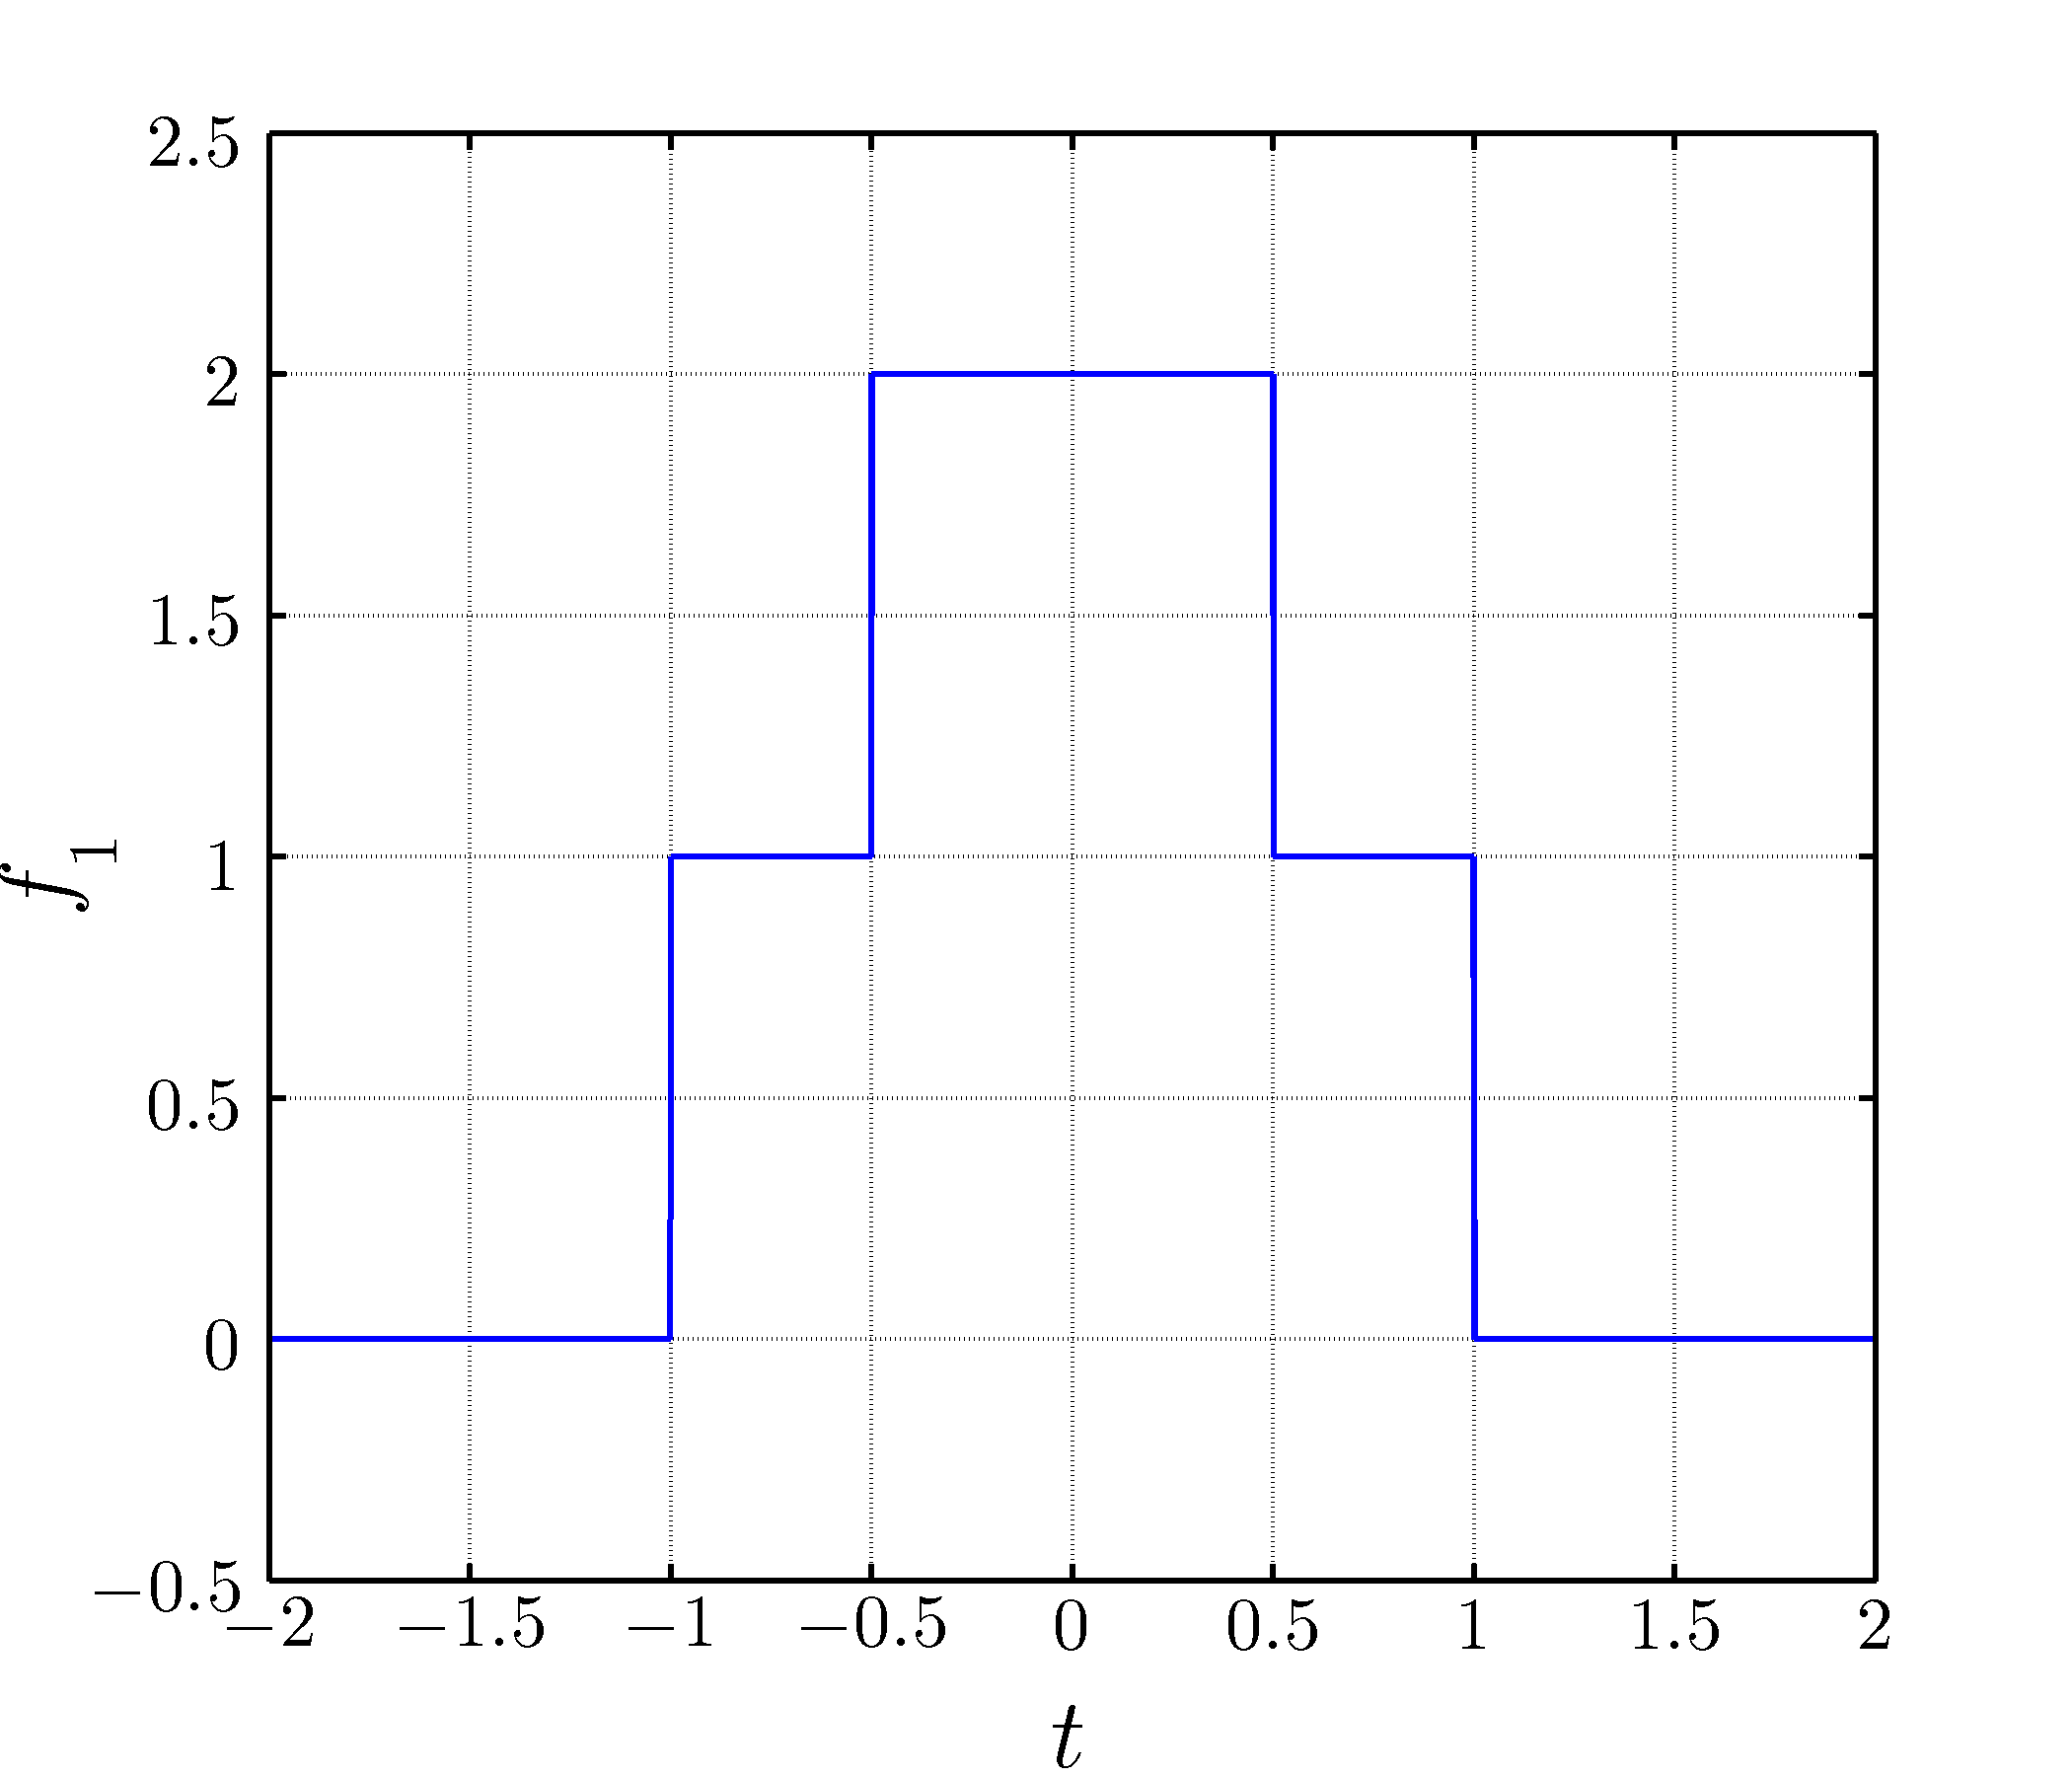
\includegraphics[width=0.45\textwidth]{./laboratorio_4/problema01_f1.png}
          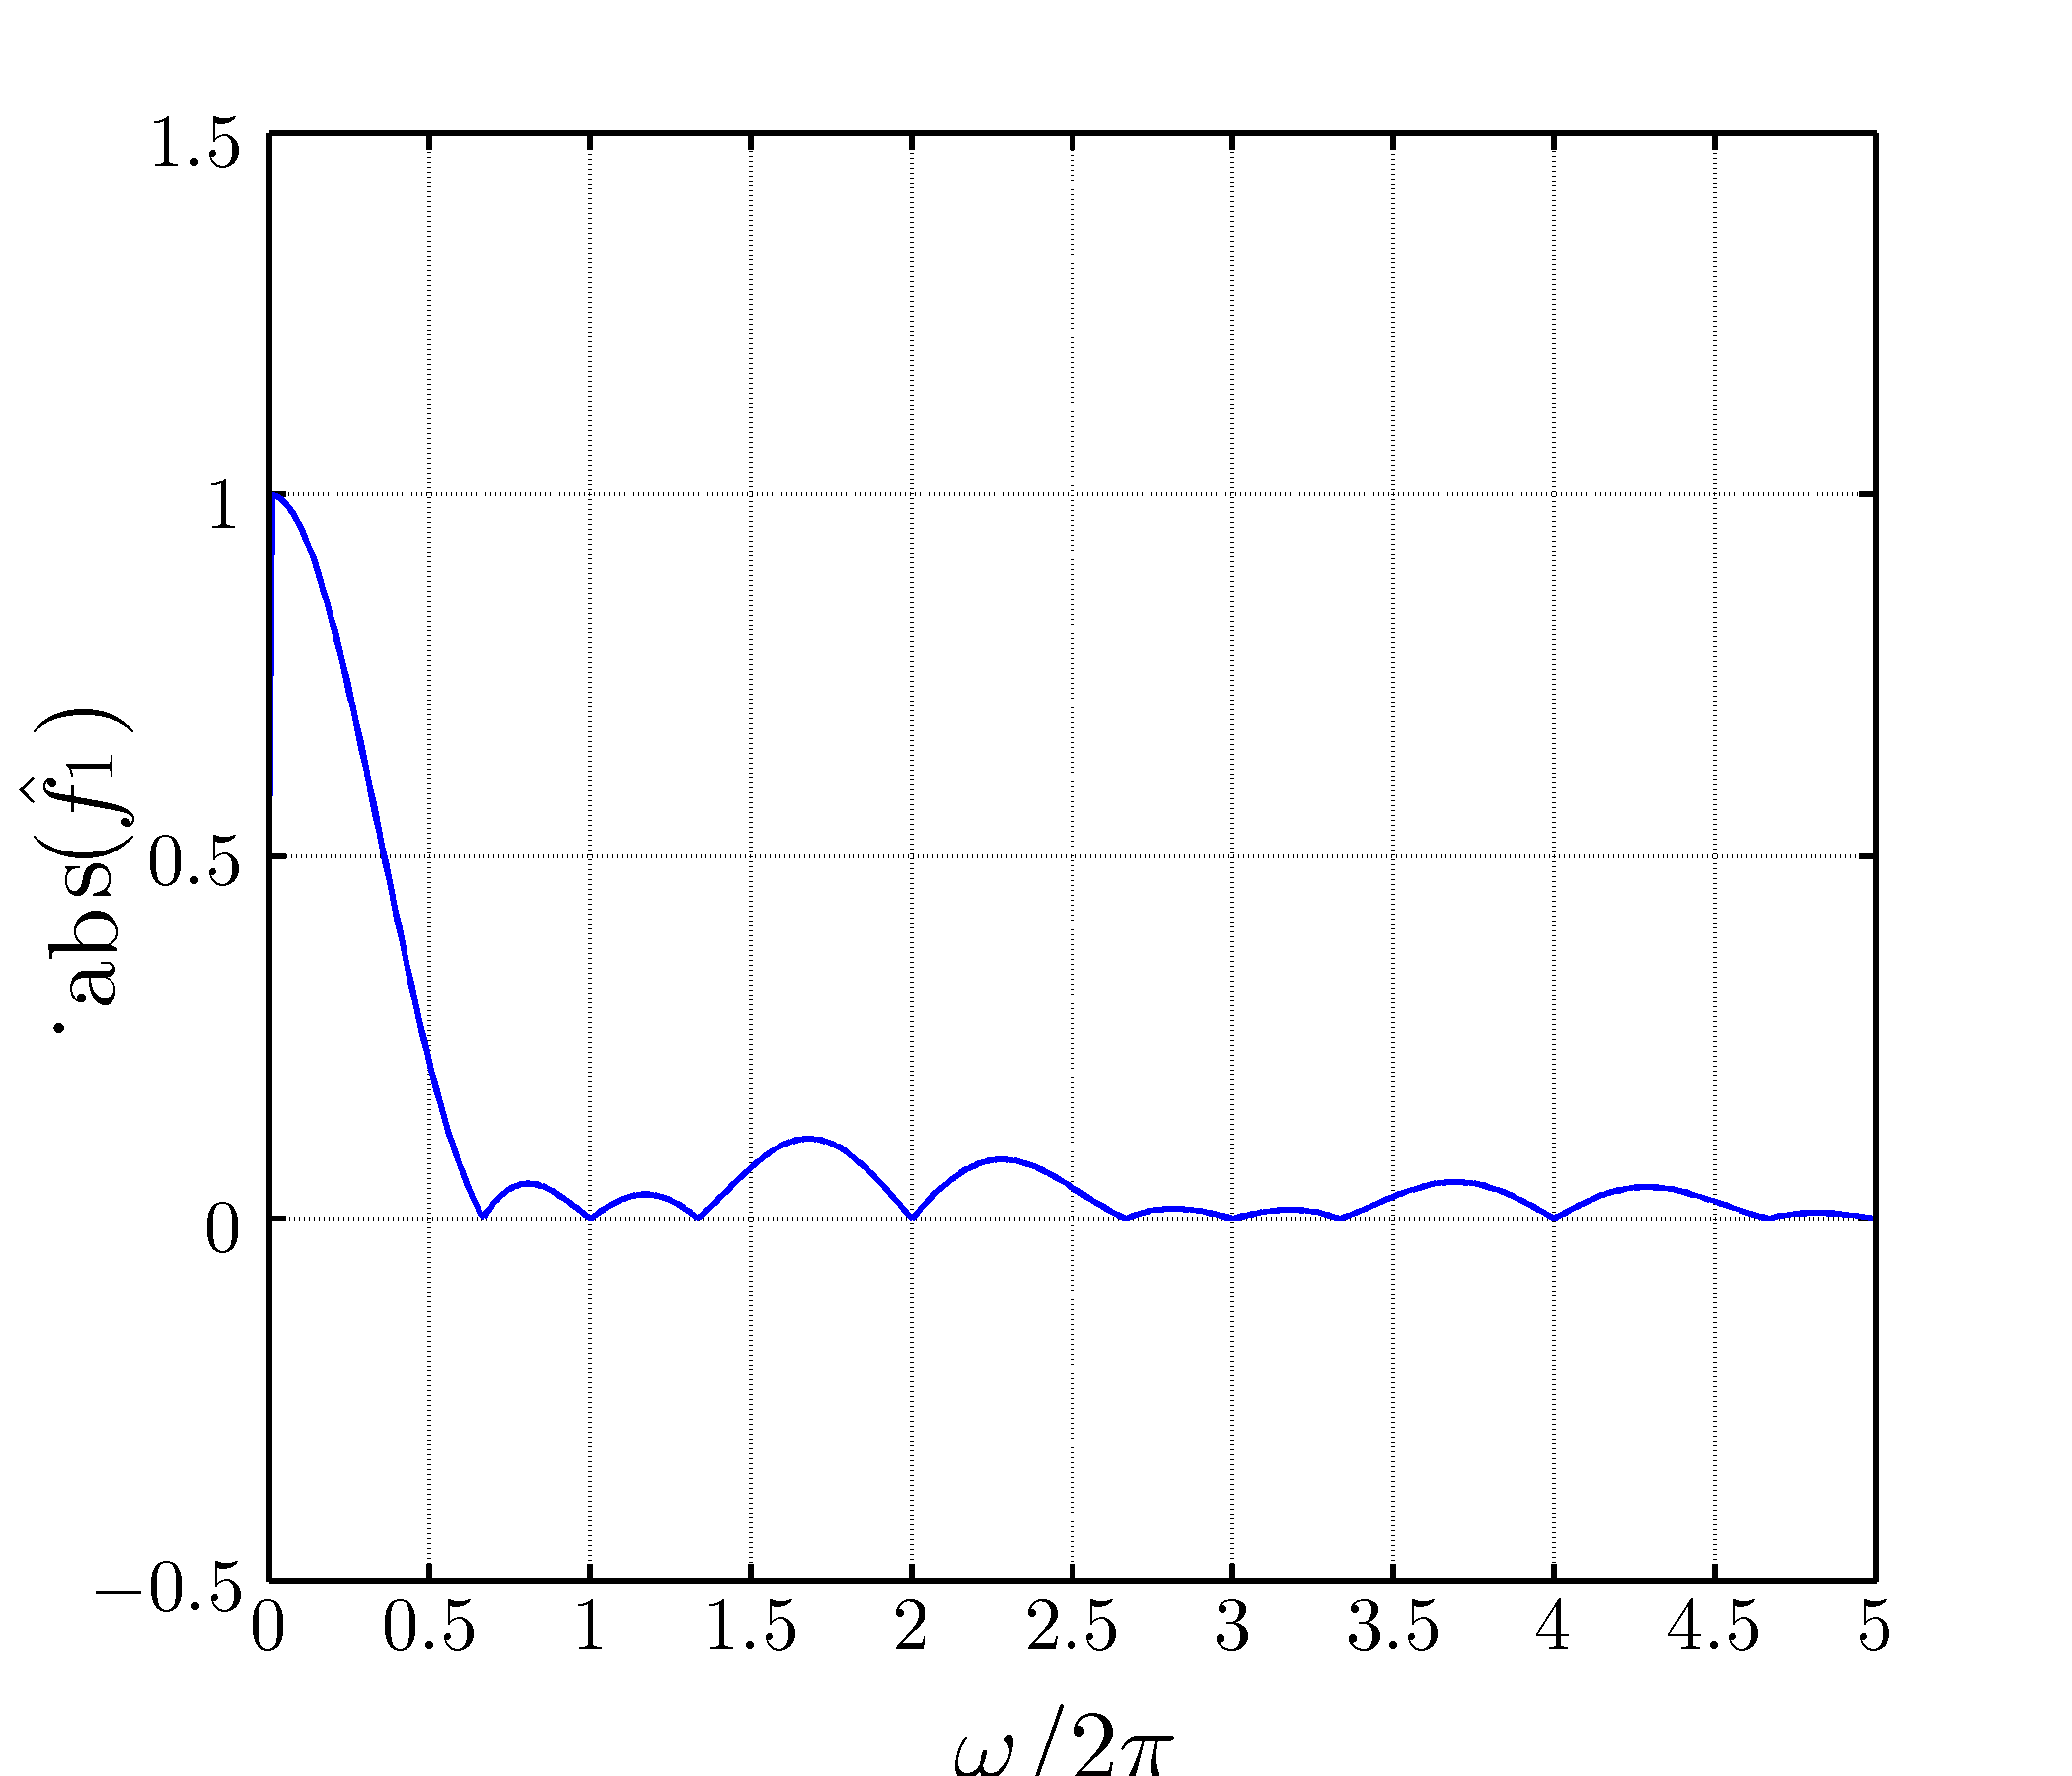
\includegraphics[width=0.45\textwidth]{./laboratorio_4/problema01_F1.png}
        \end{center}
      \end{figure}

      \begin{figure}[H]
        \caption{Gráfico de la función $f_2$ y su espectro de potencia normalizado.}
        \label{script01Bfigure}
        \begin{center}
          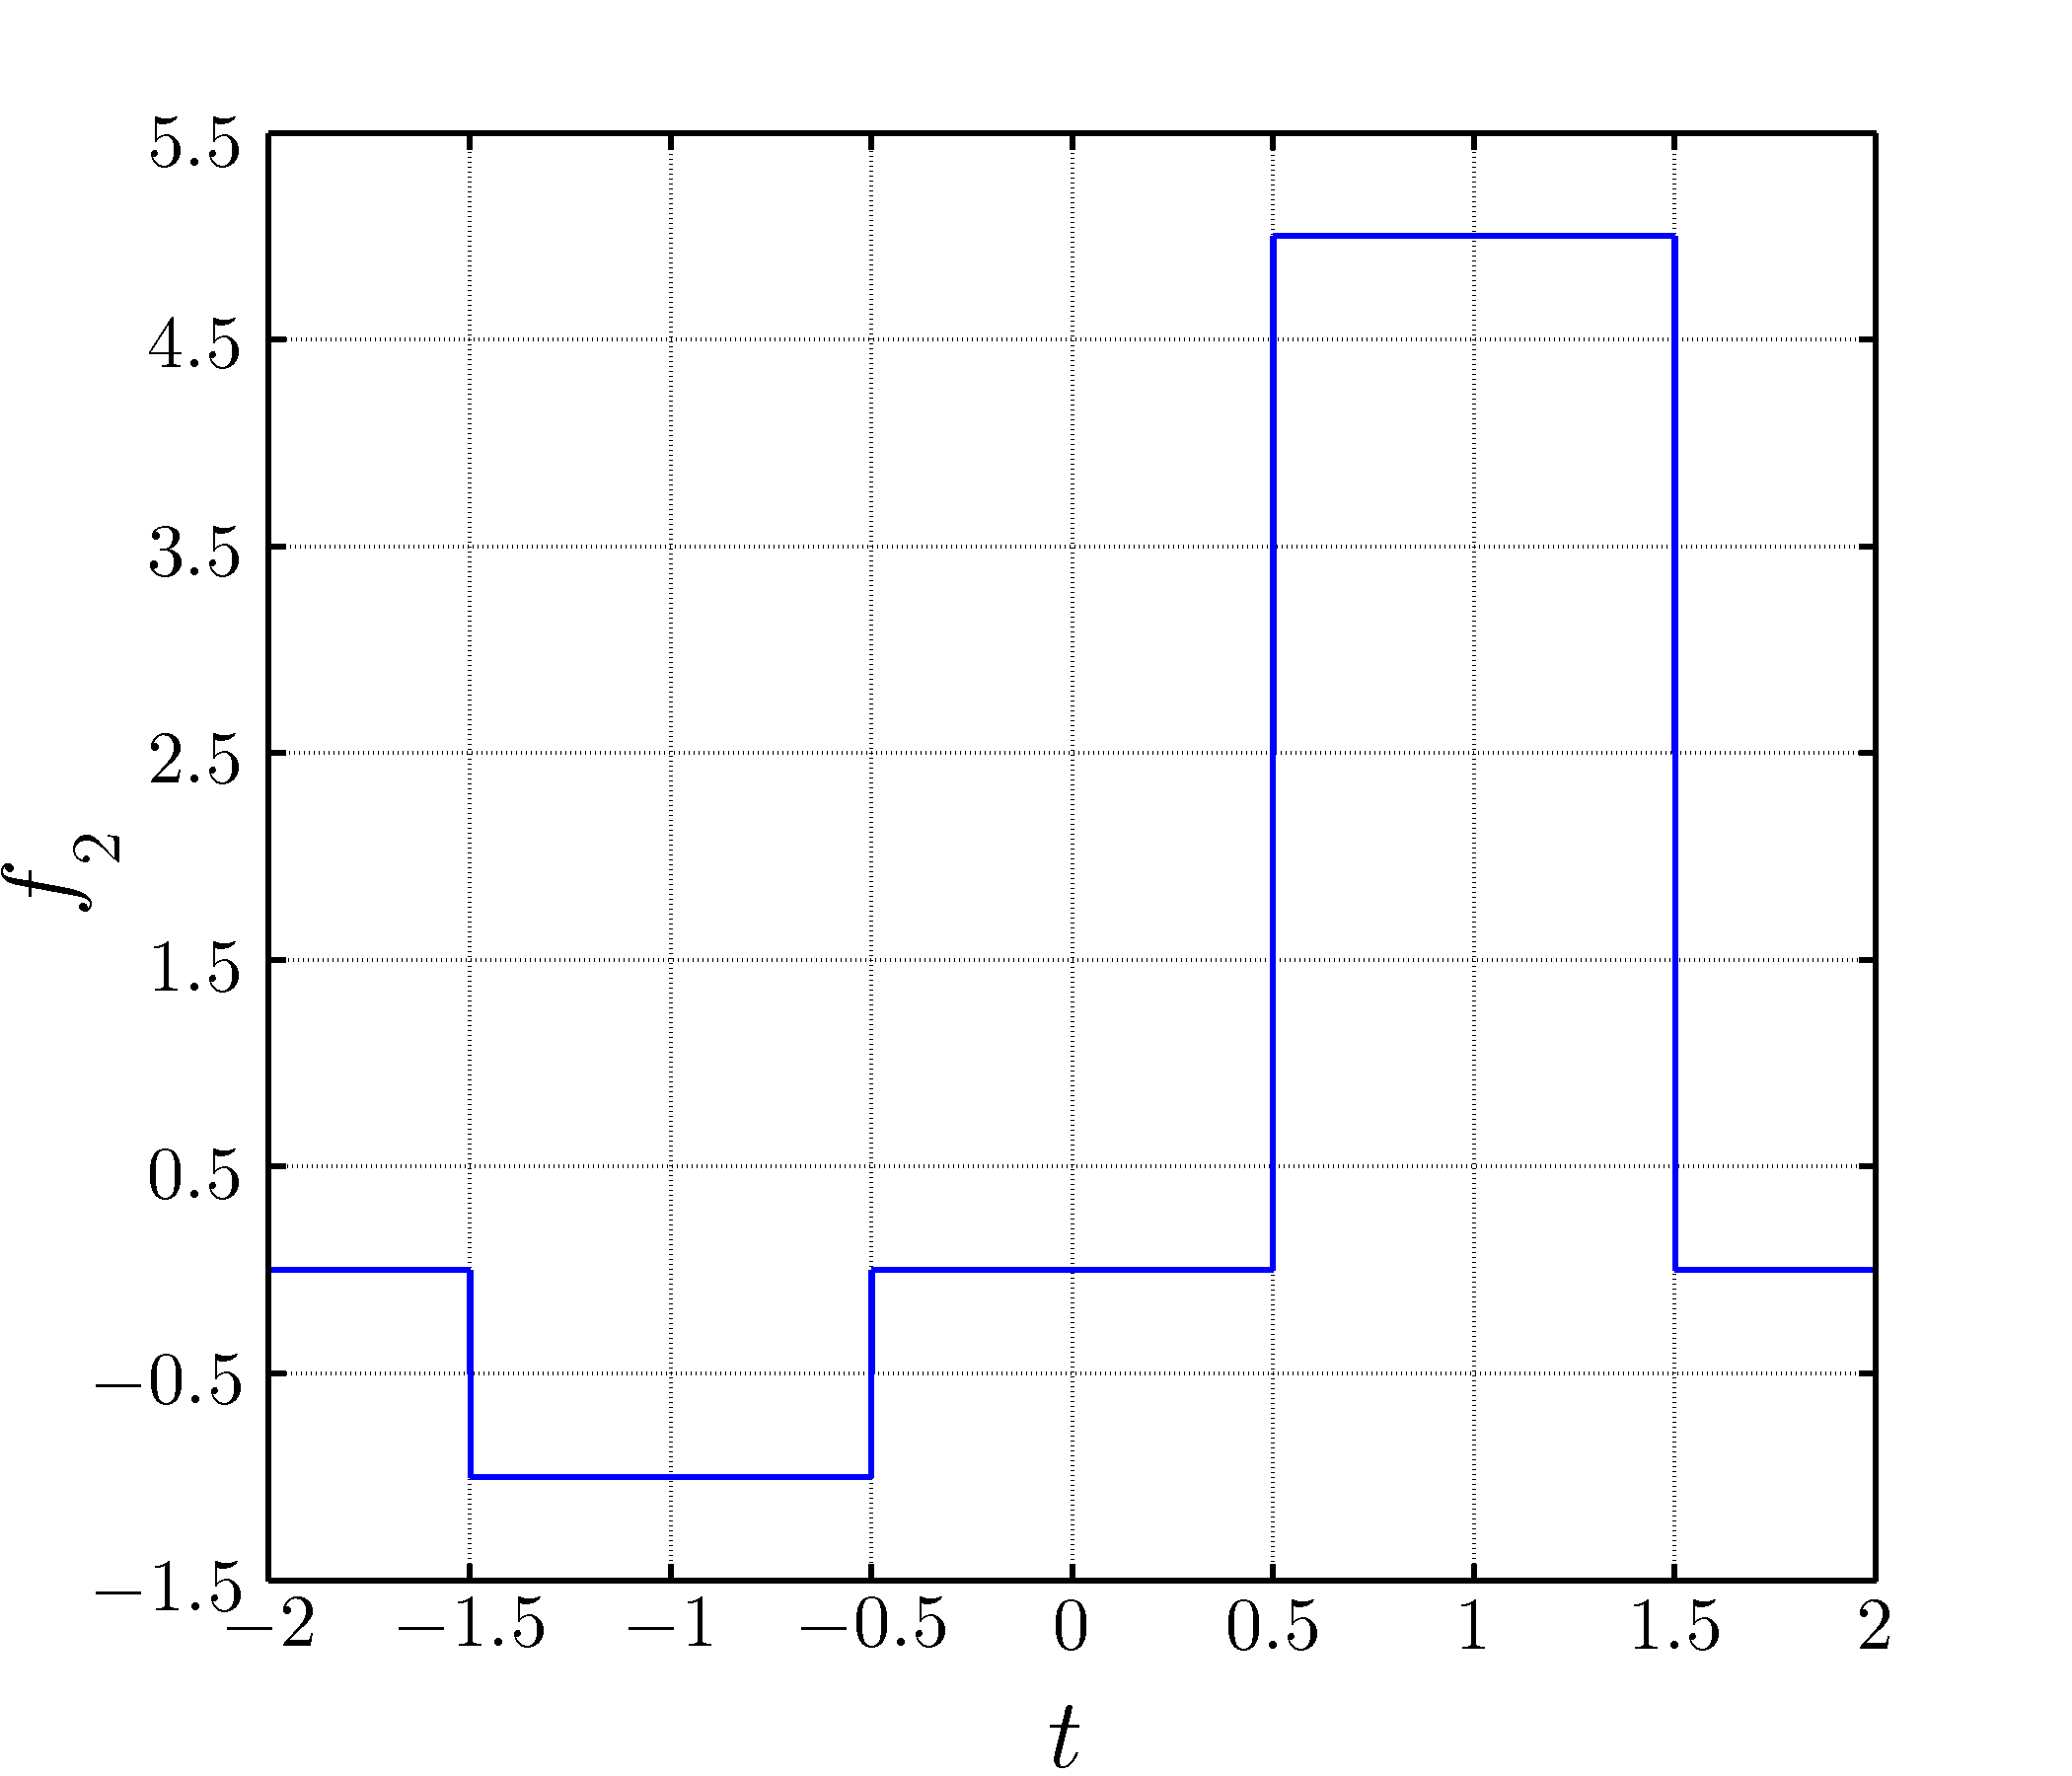
\includegraphics[width=0.45\textwidth]{./laboratorio_4/problema01_f2.png}
          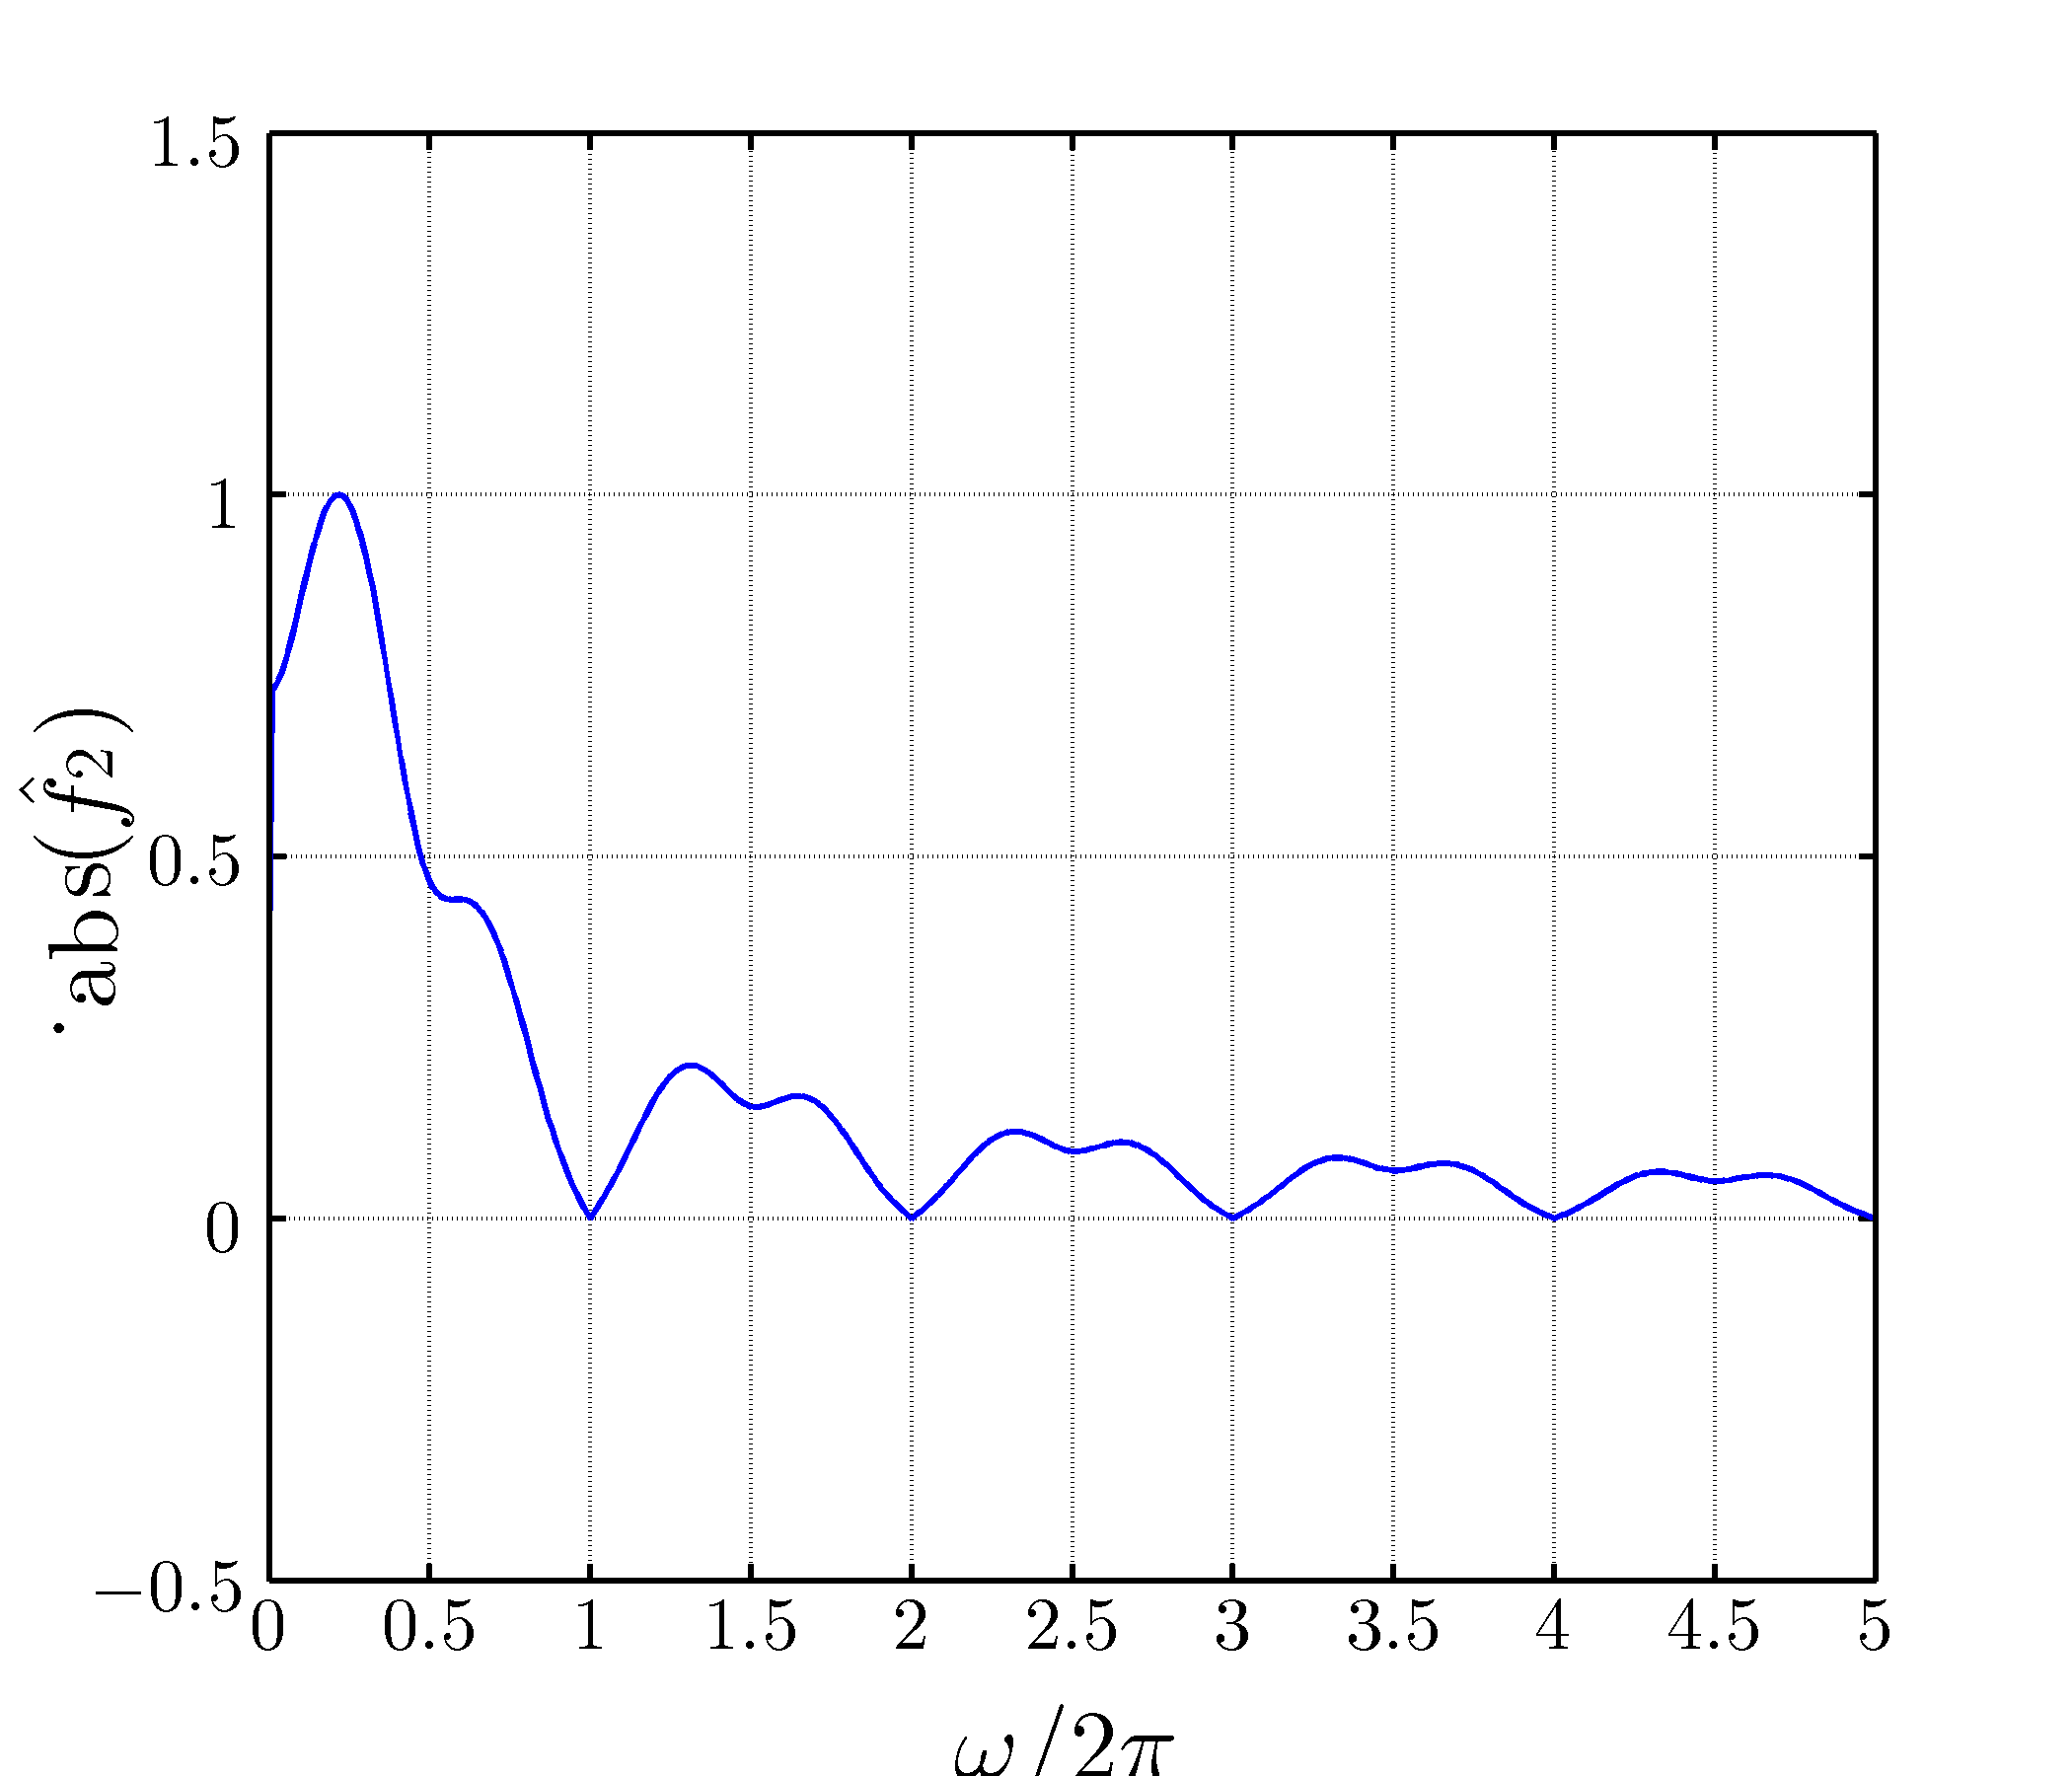
\includegraphics[width=0.45\textwidth]{./laboratorio_4/problema01_F2.png}
        \end{center}
      \end{figure}

      \begin{figure}[H]
        \caption{Gráfico de la función $f_3$ y su espectro de potencia normalizado.}
        \label{script01Cfigure}
        \begin{center}
          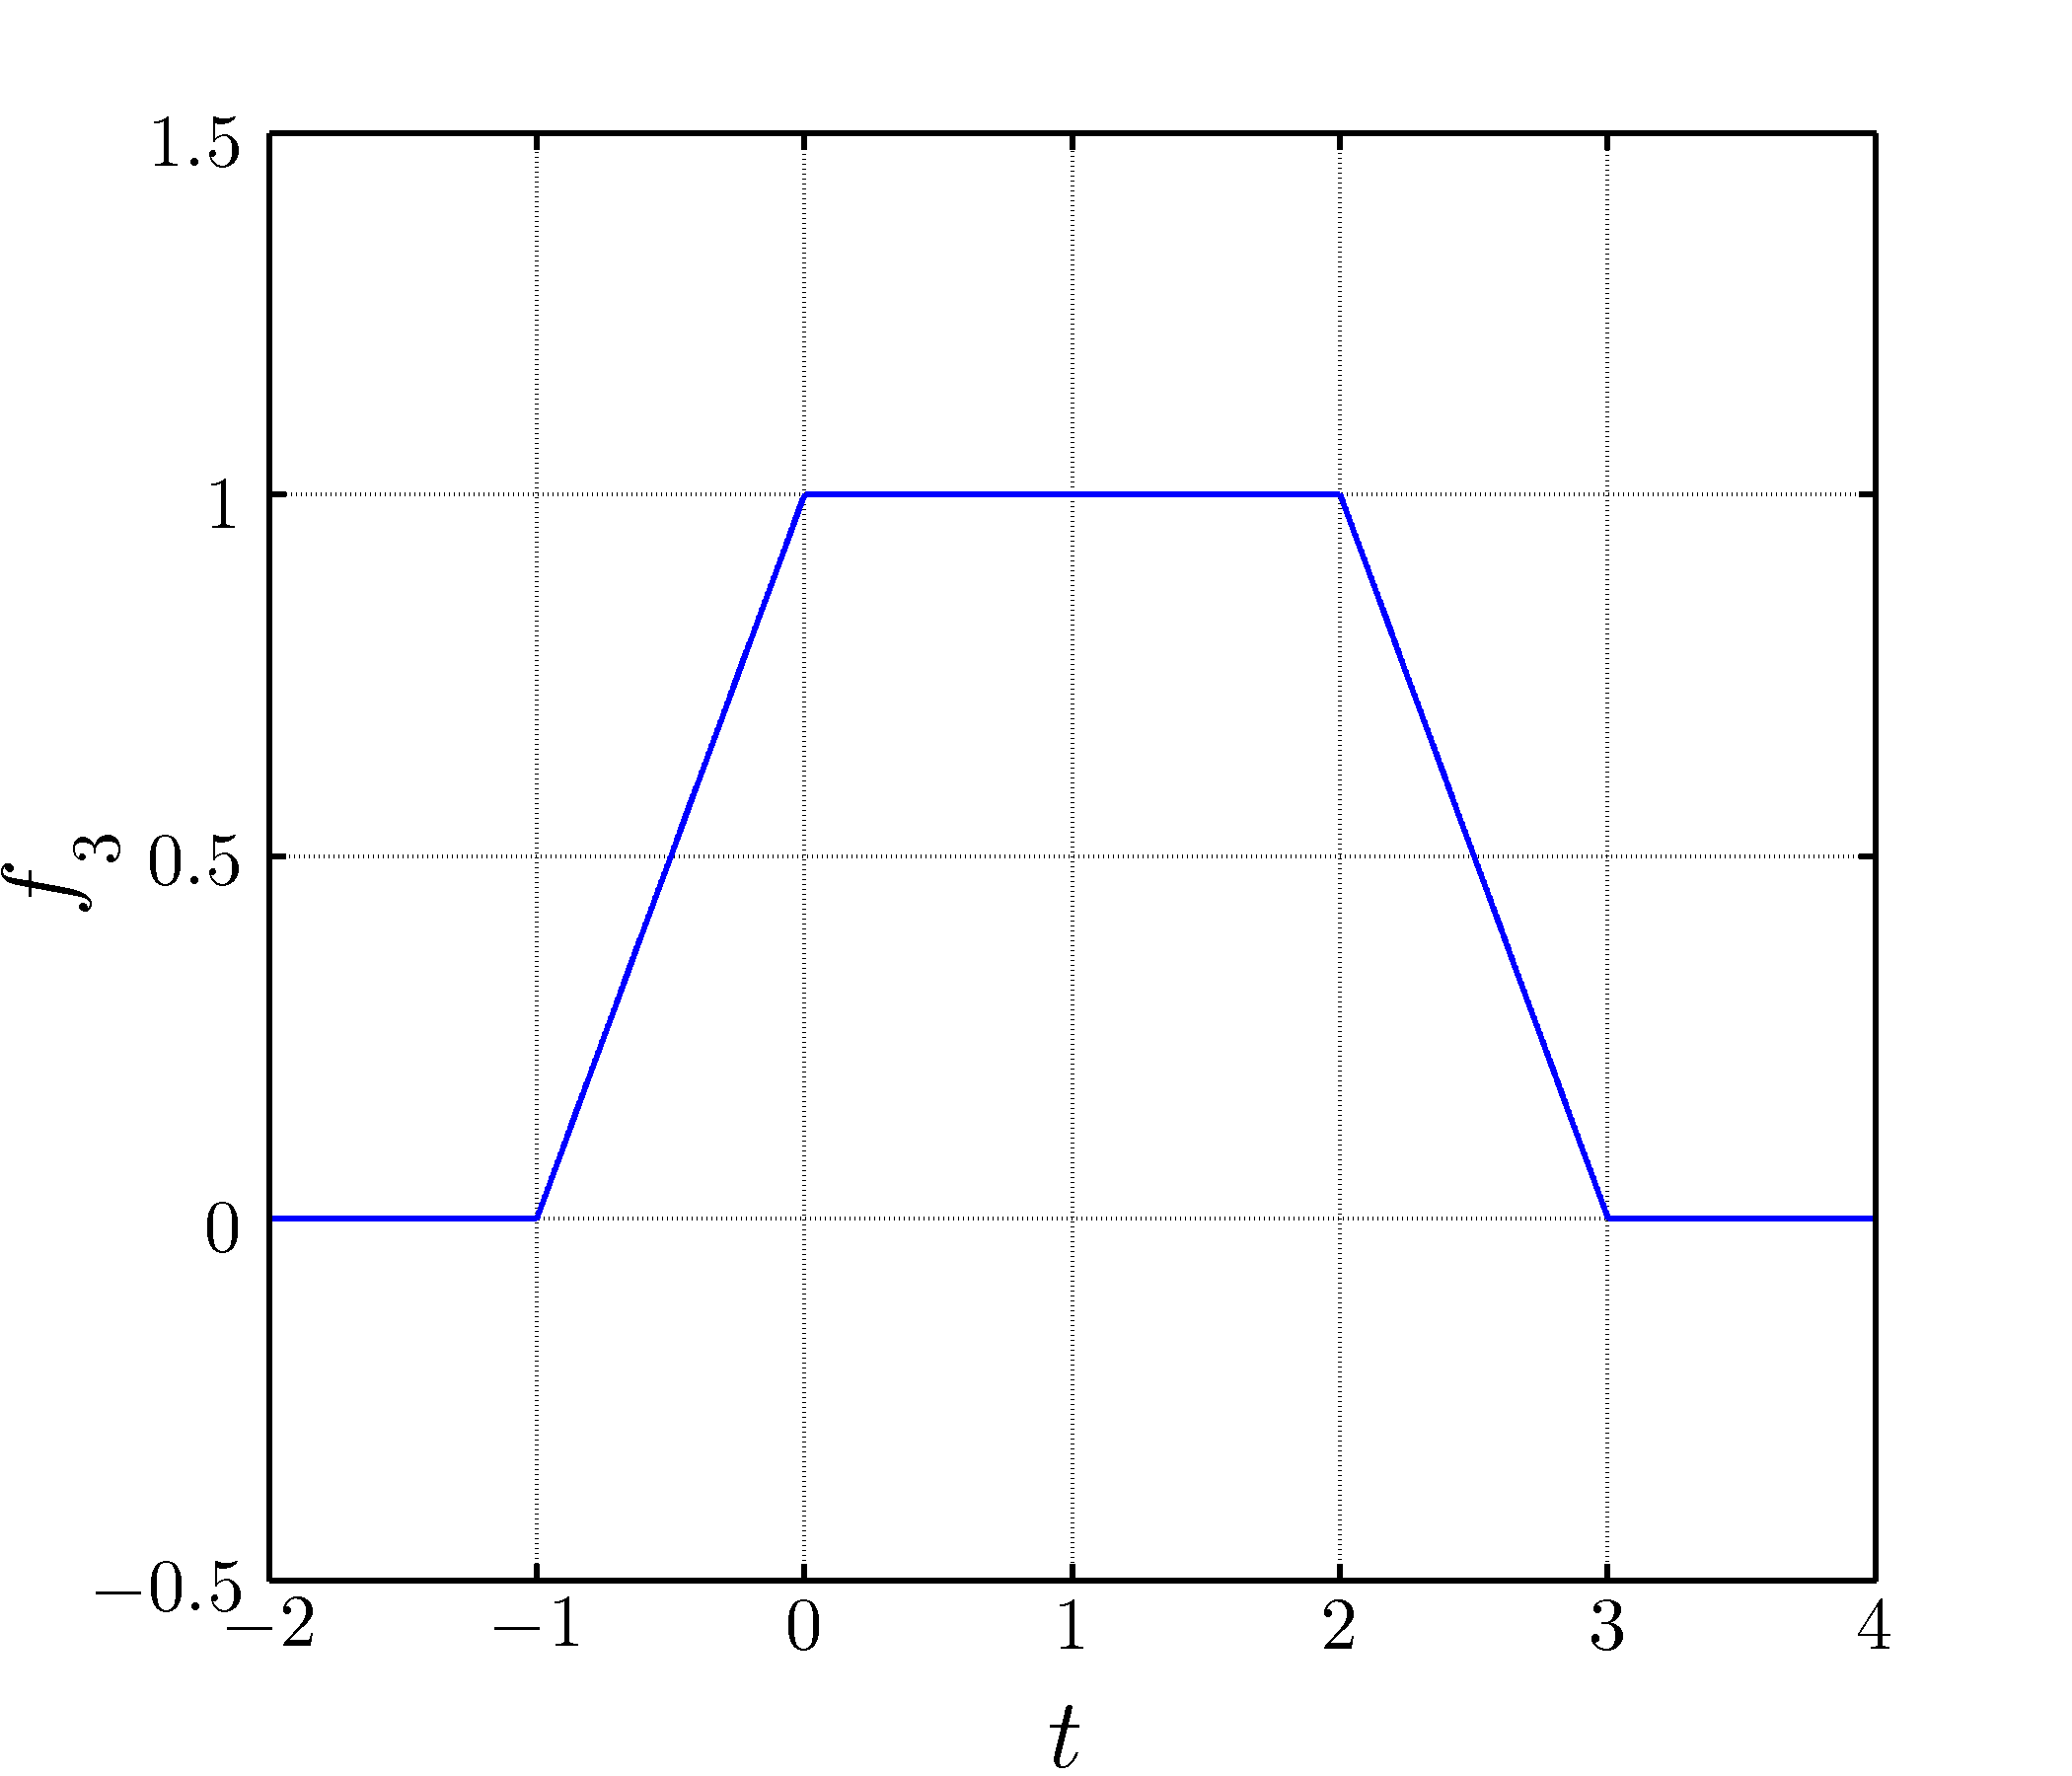
\includegraphics[width=0.45\textwidth]{./laboratorio_4/problema01_f3.png}
          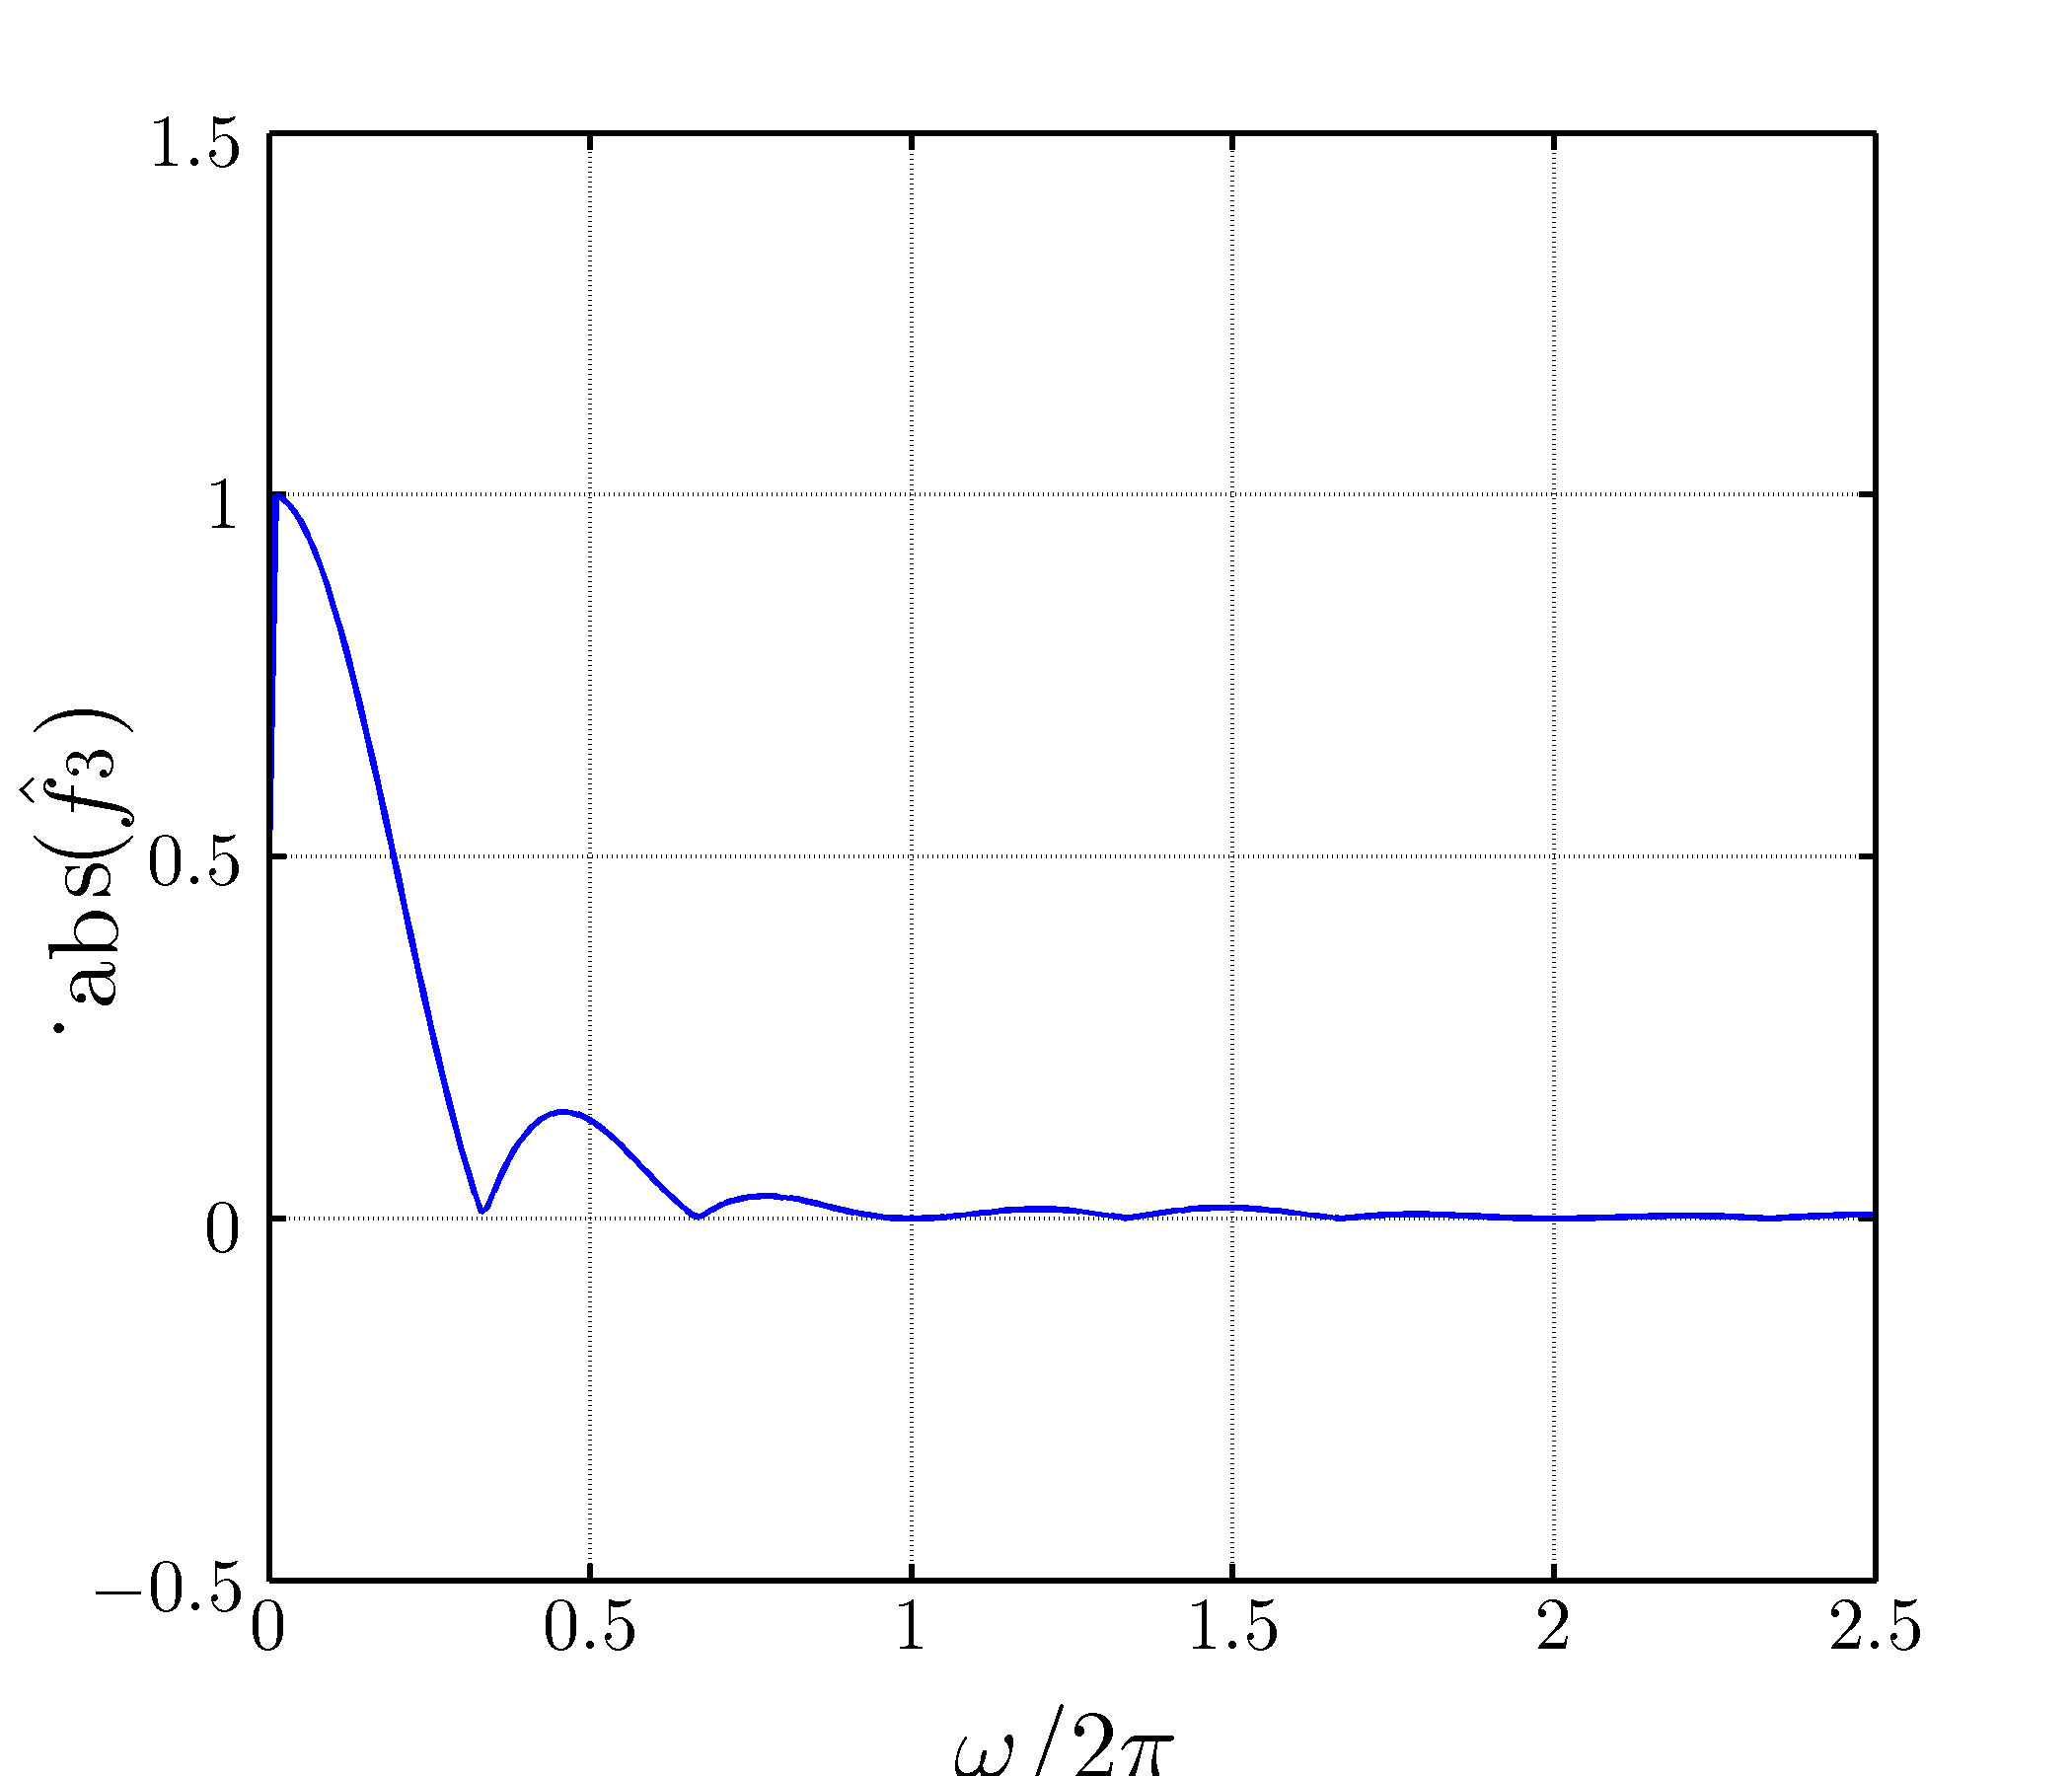
\includegraphics[width=0.45\textwidth]{./laboratorio_4/problema01_F3.png}
        \end{center}
      \end{figure}

      \begin{figure}[H]
        \caption{Gráfico de la función $f_1$ y su espectro de potencia normalizado.}
        \label{script01Dfigure}
        \begin{center}
          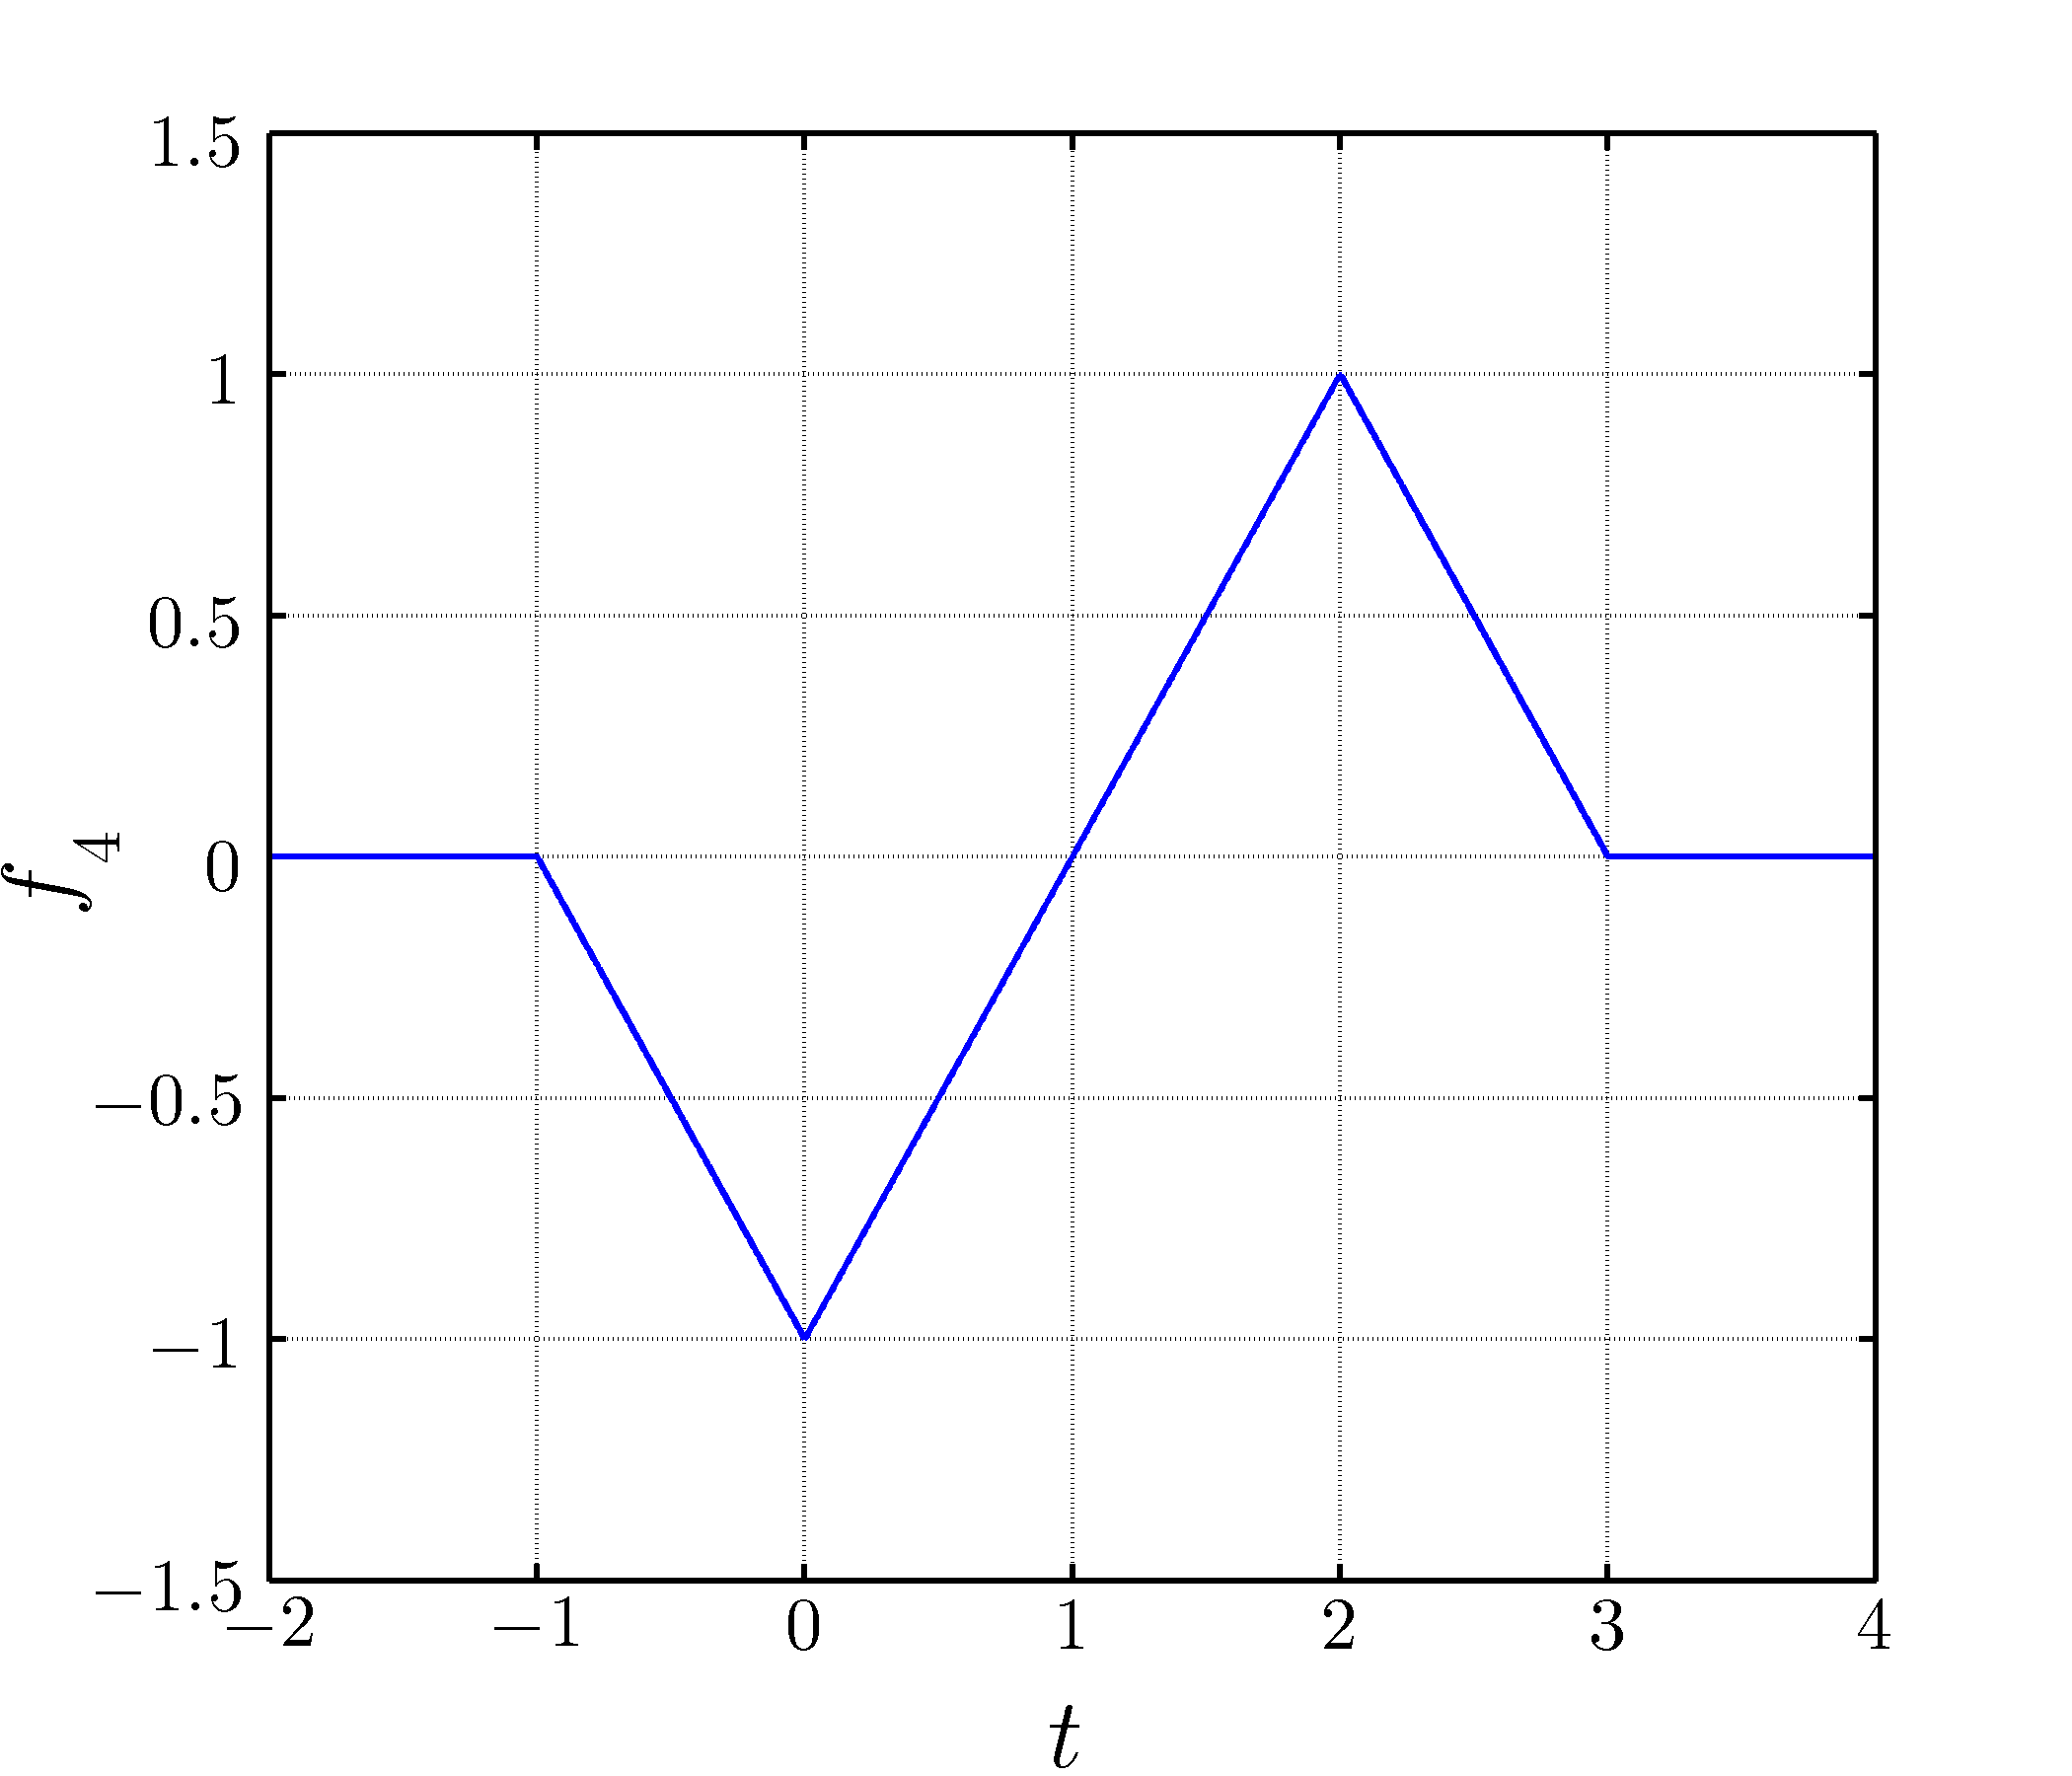
\includegraphics[width=0.45\textwidth]{./laboratorio_4/problema01_f4.png}
          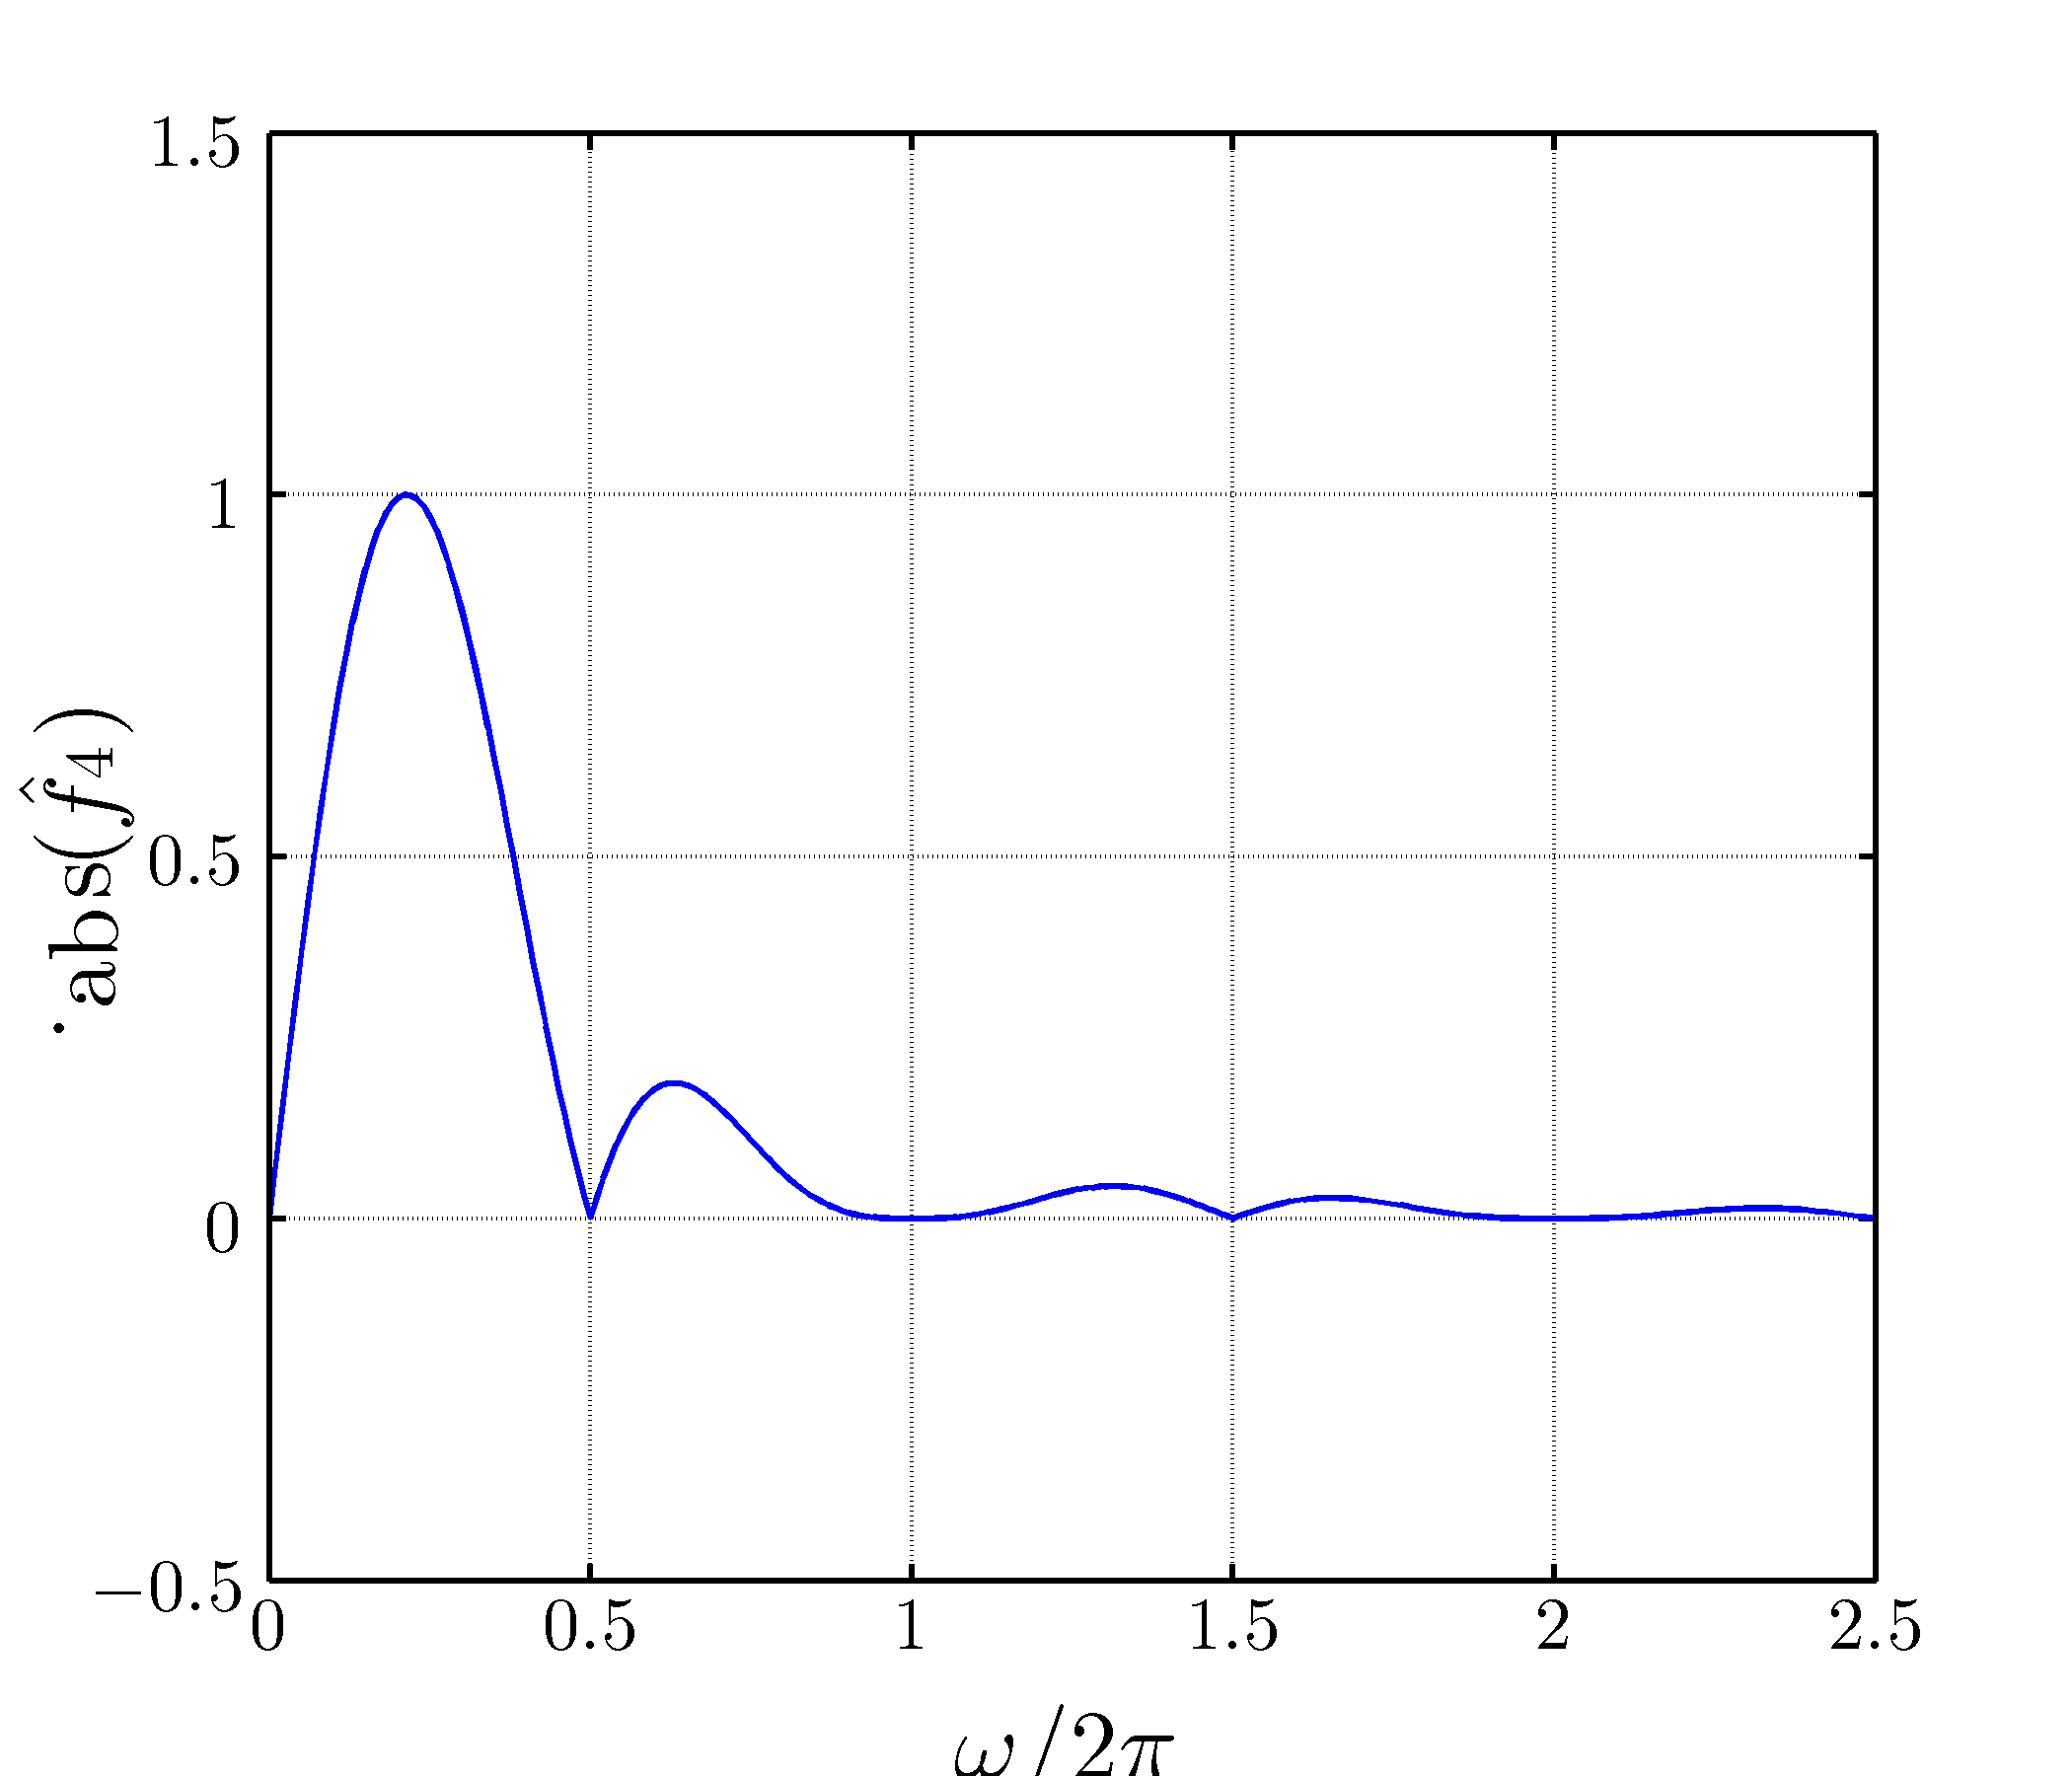
\includegraphics[width=0.45\textwidth]{./laboratorio_4/problema01_F4.png}
        \end{center}
      \end{figure}

      \begin{listing}[H]
        \caption{Script para obtener las \emph{figs. \ref{script01Afigure}, \ref{script01Bfigure}, \ref{script01Cfigure}} y \emph{\ref{script01Dfigure}.}}
        \label{script01G}
        \inputminted{matlab}{./laboratorio_4/problema01.m}
      \end{listing}\vspace{-1.0em}

  \newpage
  \subsection*{Problema 2}
    \floatsetup[figure]{
      capposition=top,
      style=plain,
    }

    \noindent Hallar la transformada de Fourier de $x\left(t\right)$ y graficar en Matlab:

      \begin{figure}[H]
        \begin{center}
          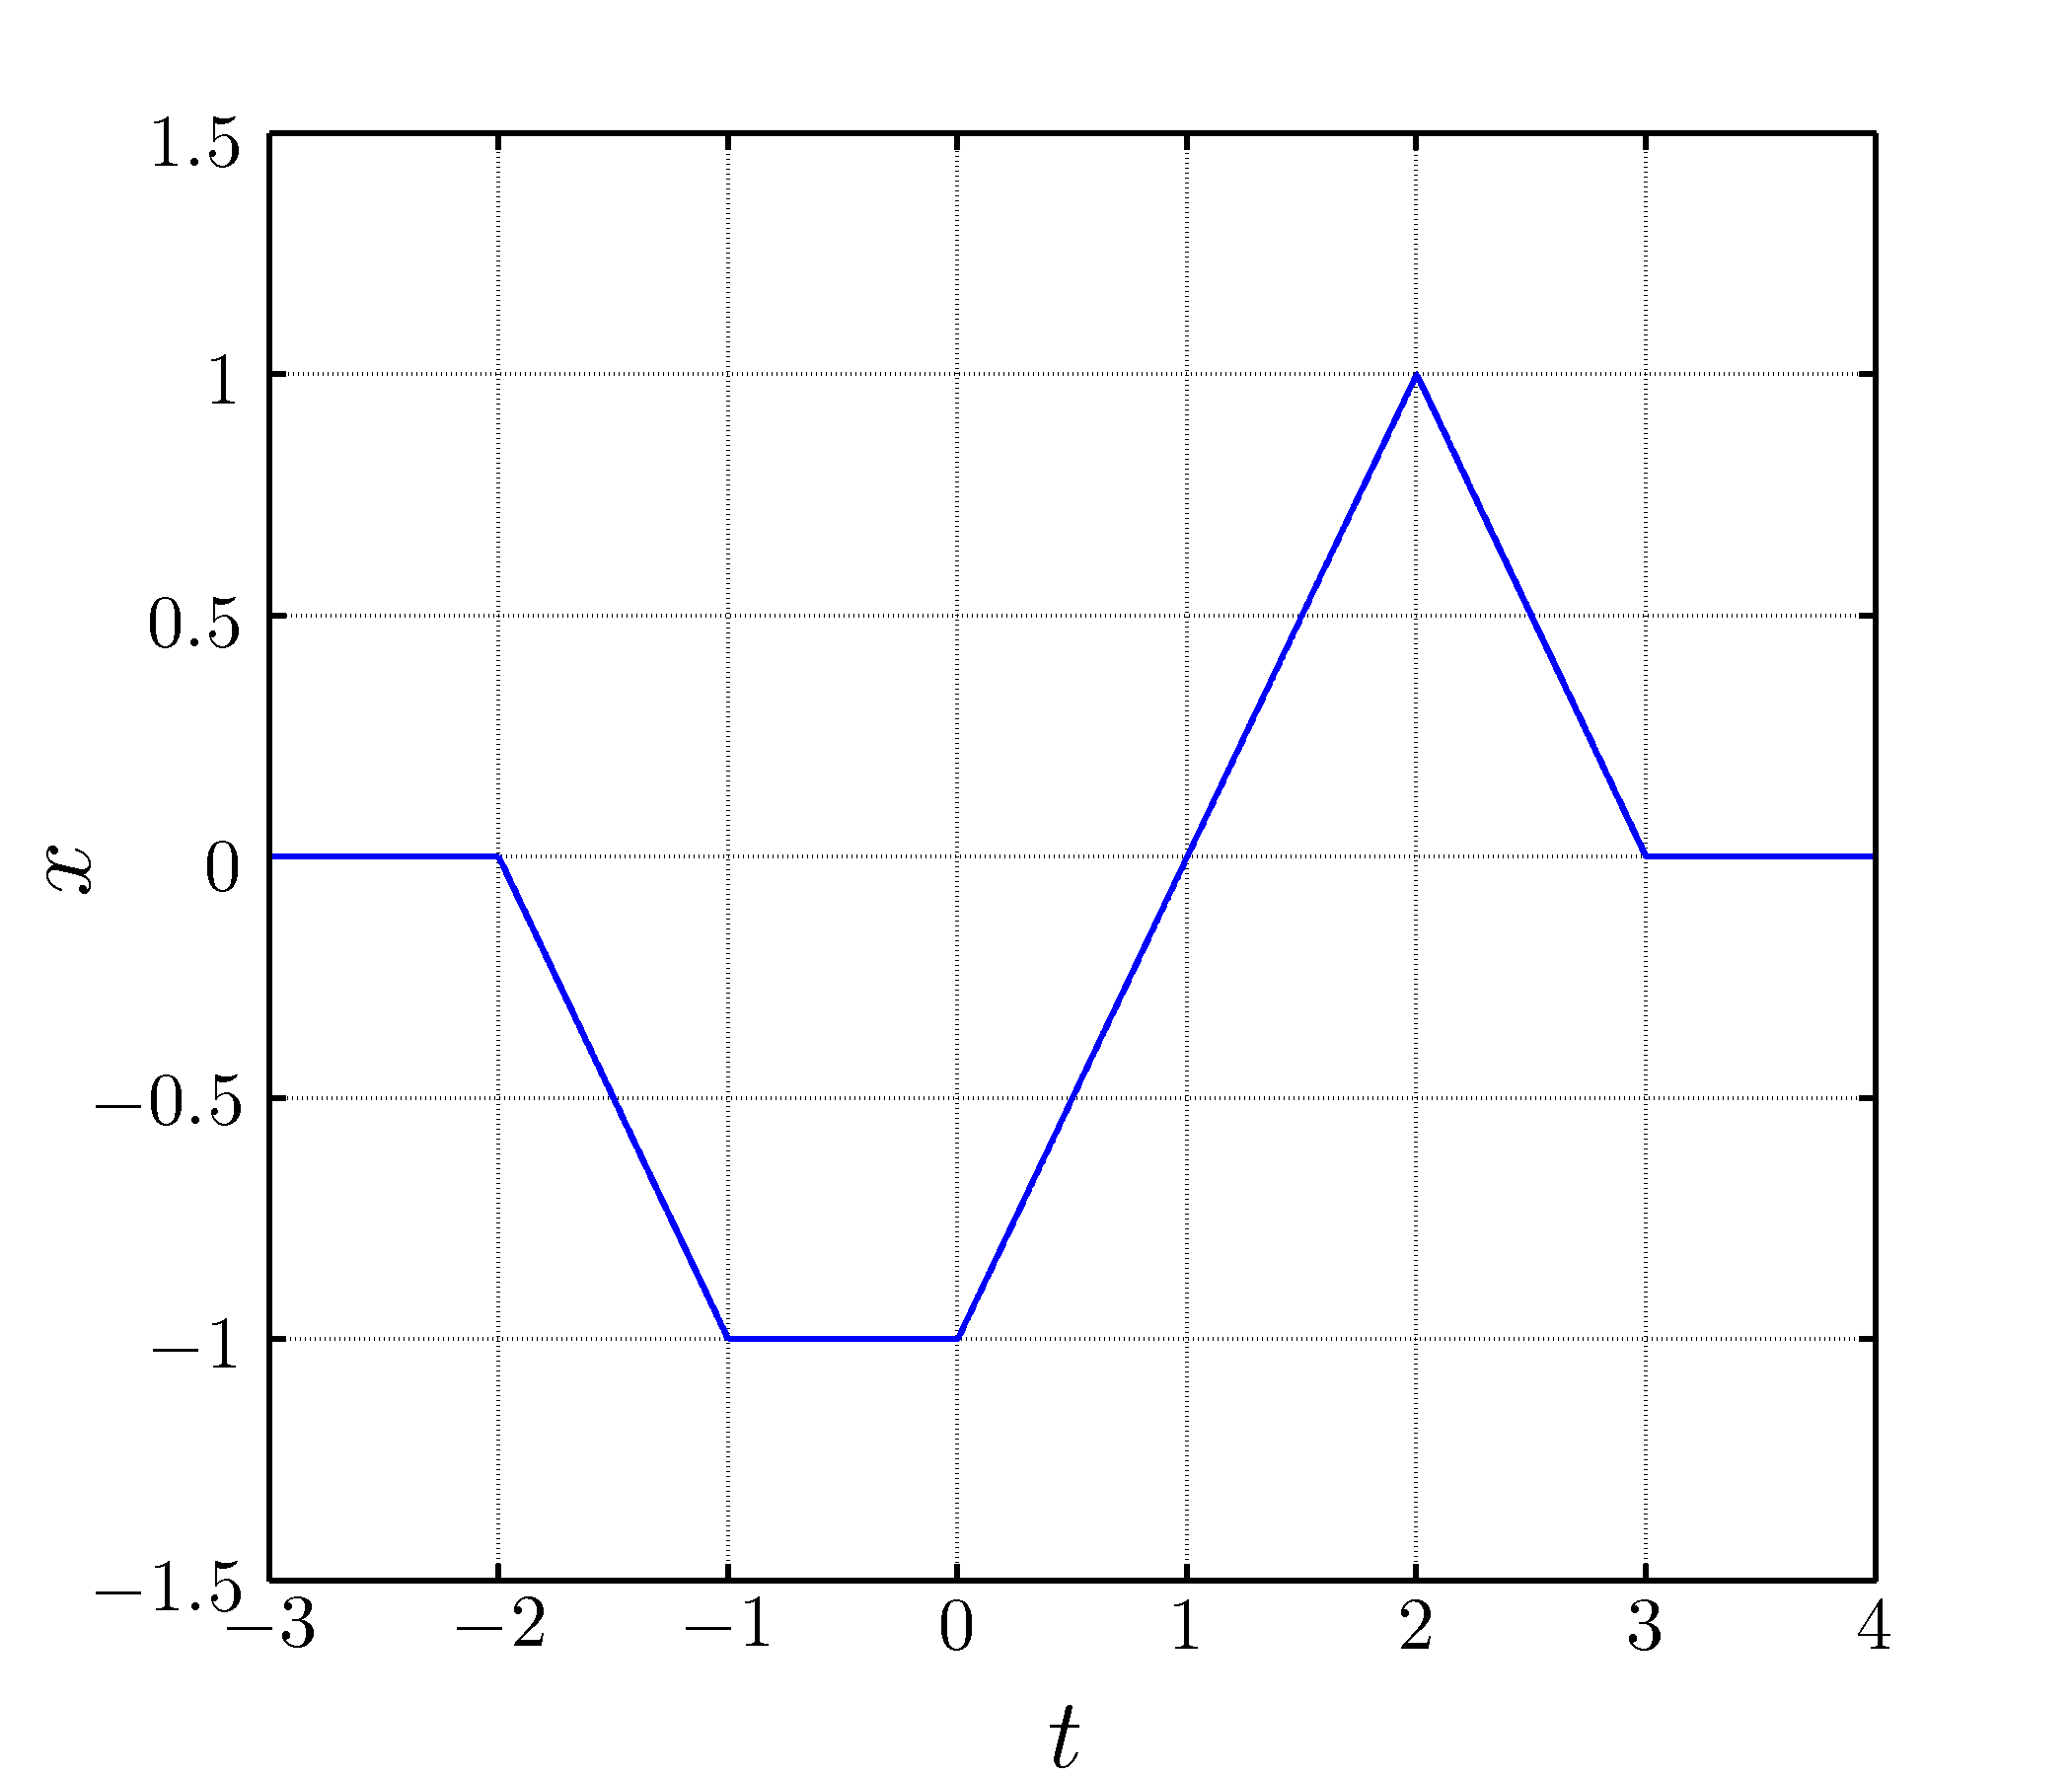
\includegraphics[width=0.45\textwidth]{./laboratorio_4/problema02_x.png}
        \end{center}
      \end{figure}

    \noindent Si $x\left(t\right)$ pasa a través del bloque de la figura,
      calcule la transformada de Fourier de $y\left(t\right)$.

      \begin{figure}[H]
        \begin{center}
          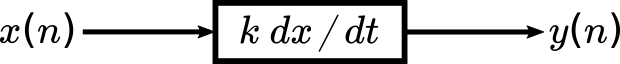
\includegraphics[width=0.45\textwidth]{./laboratorio_4/problema02_diagram.png}
        \end{center}
      \end{figure}\vspace{-1.5em}

    \subsubsection*{Solución}
      \floatsetup[figure]{
        capposition=top,
        style=ruled,
      }

      \noindent La función $x\left(t\right)$ se puede modelar empleando la función triángulo como

        \begin{equation*}
         x\left(t\right) = - \Lambda\left(t + 1\right)
                           - \Lambda\left(t \right)
                           + \Lambda\left(t - 2\right).
        \end{equation*}

      \noindent Así, la transformada de fourier vendrá dada por:

        \begin{equation*}
          \begin{split}
            \widehat{f}\left(\omega\right) & = - \mathcal{F}\left(\Lambda,t + 1|\omega\right) - \mathcal{F}\left(\Lambda,t|\omega\right) + \mathcal{F}\left(\Lambda,t - 2|\omega\right) \\
                                           & = - \mathcal{F}\left(\Lambda,t + 1|\omega\right) - \mathcal{F}\left(\Lambda,t|\omega\right) + \mathcal{F}\left(\Lambda,t - 2|\omega\right) \\
                                           & = - \exp\left(i \omega\right) \mathcal{F}\left(\Lambda,t|\omega\right) - \mathcal{F}\left(\Lambda,t|\omega\right) + \exp\left(- 2 i \omega\right) \mathcal{F}\left(\Lambda,t|\omega\right) \\
                                           & = \left( - \exp\left(i \omega\right) - 1 + \exp\left(- 2 i \omega\right) \right) \mathrm{sinc}^{2}\left(\frac{\omega}{2}\right)
          \end{split}
        \end{equation*}

      \noindent En \textsc{Matlab} implementamos la función $x\left(t\right)$
        en términos de la función triángulo tal como muestra el \emph{script
        \ref{script02A}} y calculamos su espectro de potencia según el
        \emph{script \ref{script02B}} para obtner la \emph{figura
        \ref{script02Afigure}}

        \begin{listing}[H]
          \caption{Función $x\left(t\right)$.}
          \label{script02A}
          \inputminted{matlab}{./laboratorio_4/p2_x.m}
        \end{listing}

        \begin{listing}[H]
          \caption{Función $x\left(t\right)$.}
          \label{script02B}
          \inputminted{matlab}{./laboratorio_4/problema02.m}
        \end{listing}

      \begin{figure}[H]
          \caption{Función $x\left(t\right)$ y espectro su espectro de potencia normalizado.}
          \label{script02Afigure}
          \begin{center}
              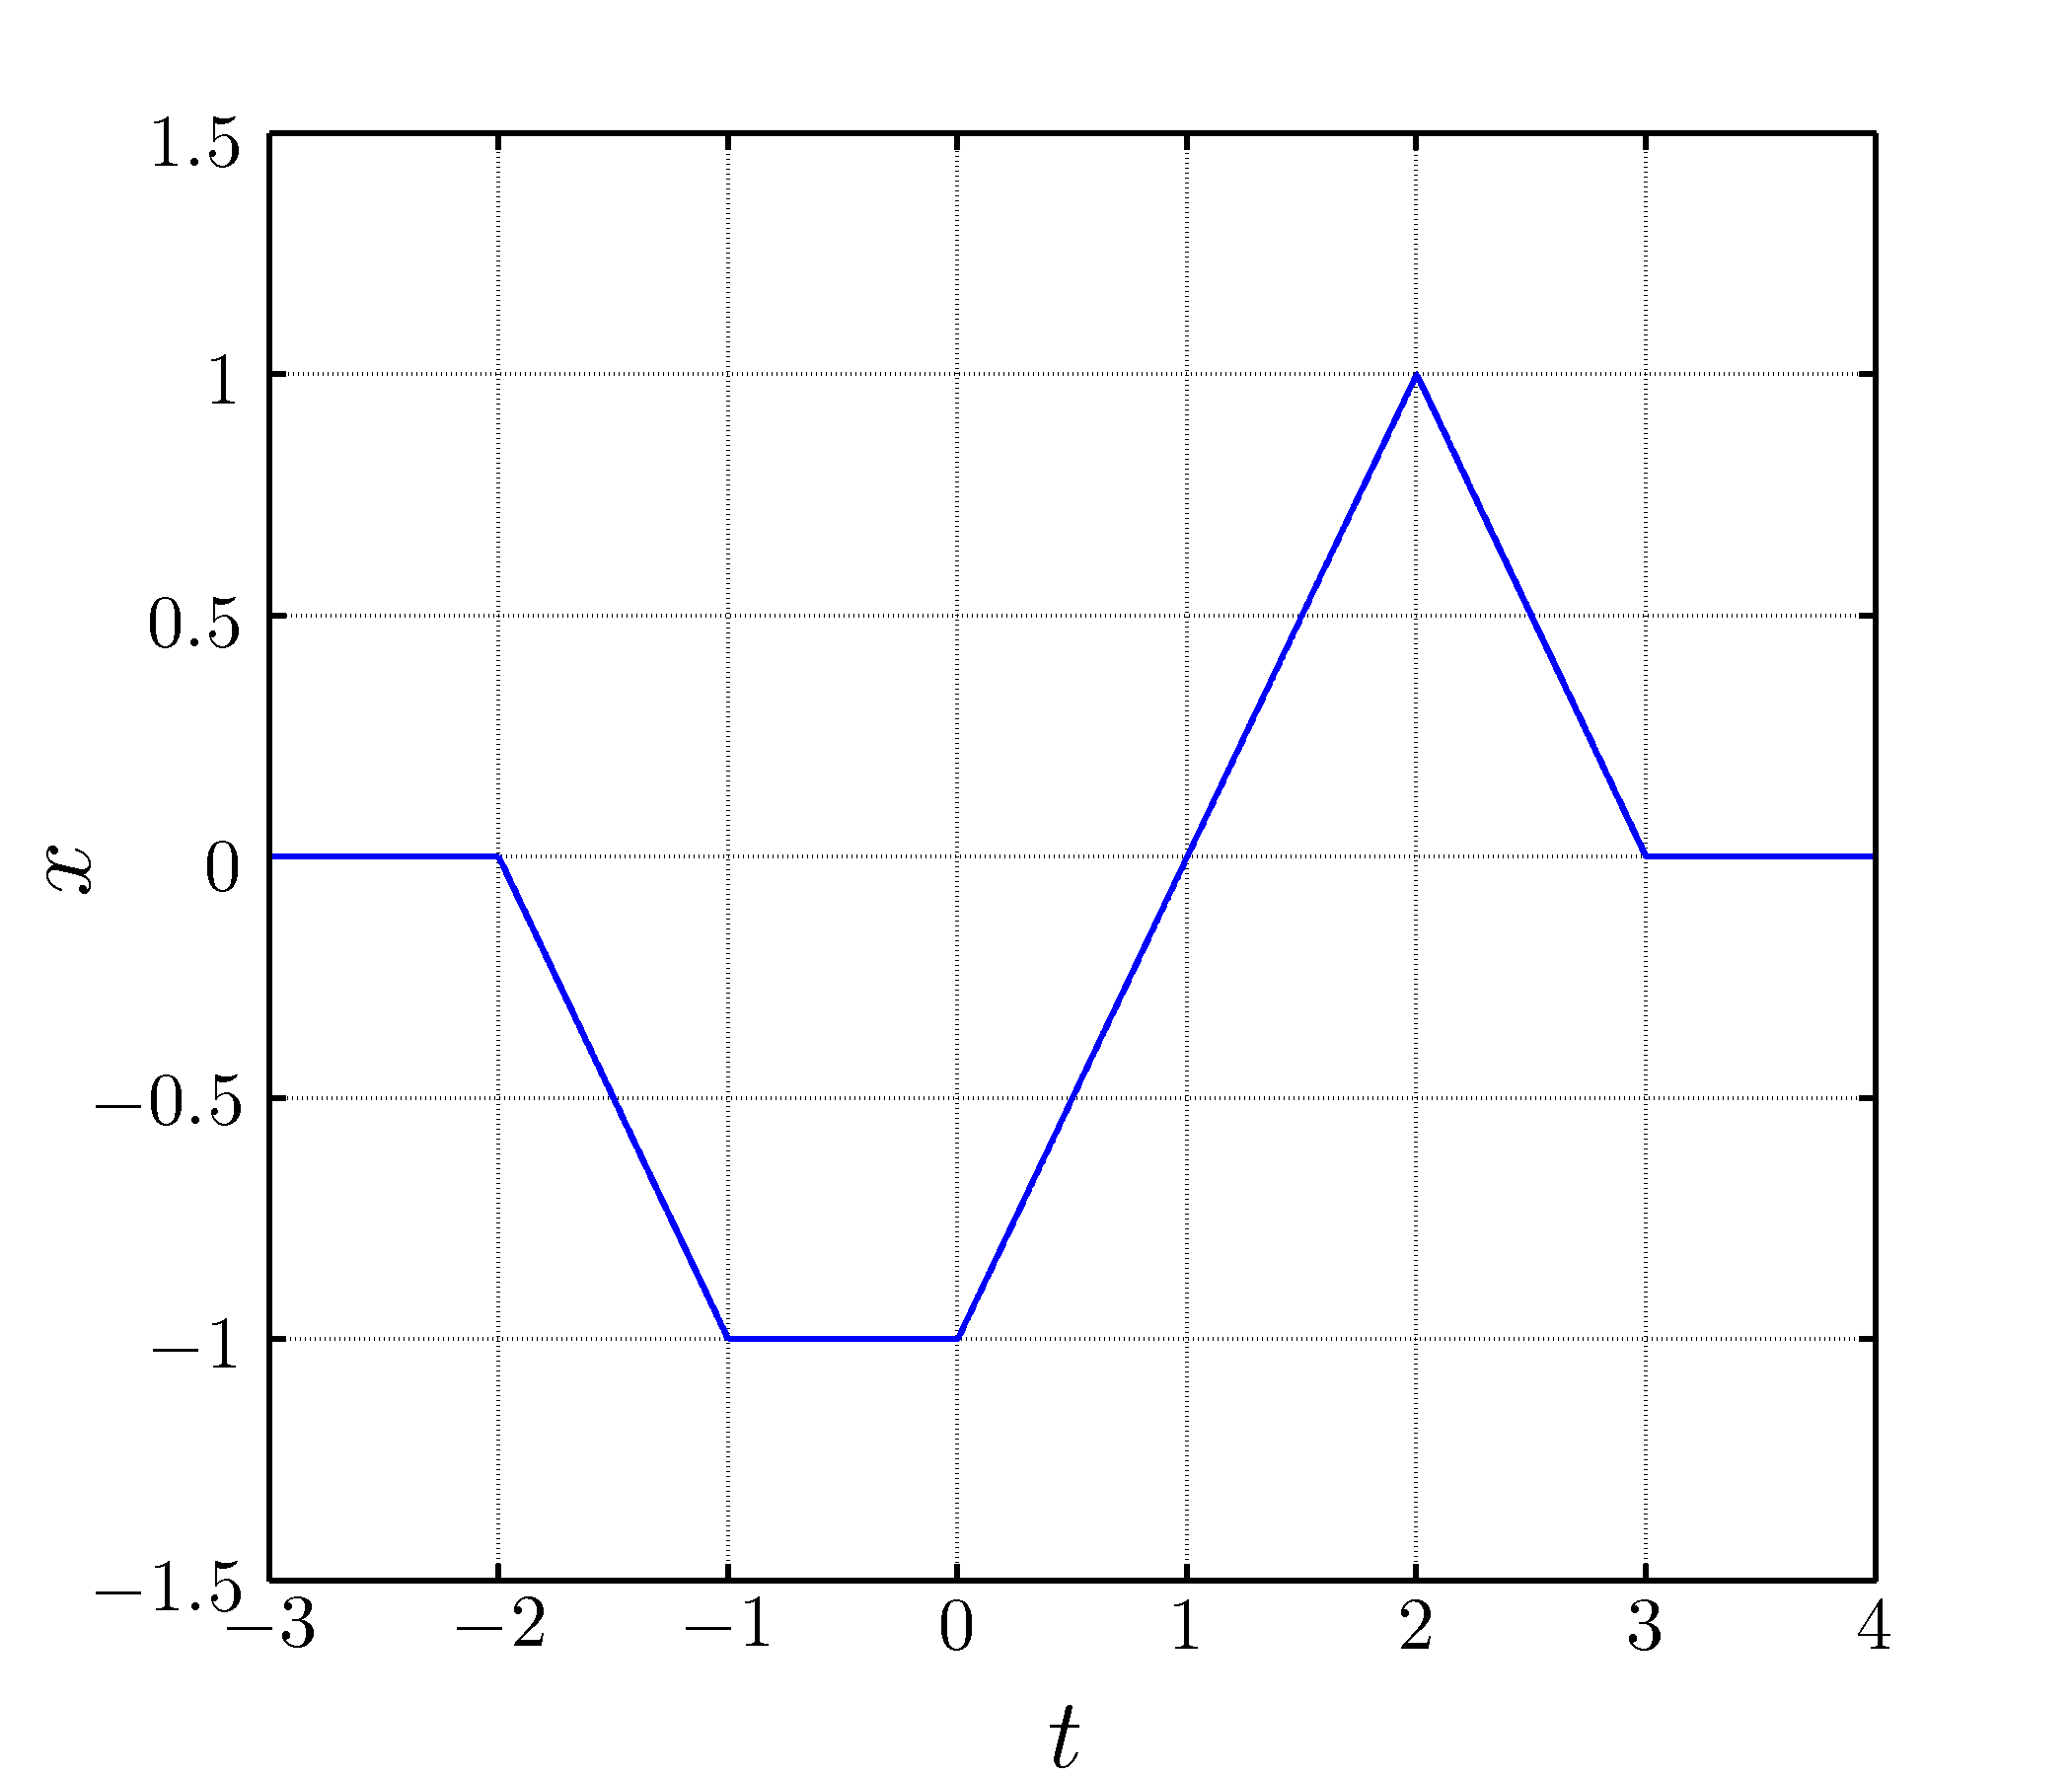
\includegraphics[width=0.45\textwidth]{./laboratorio_4/problema02_x.png}
              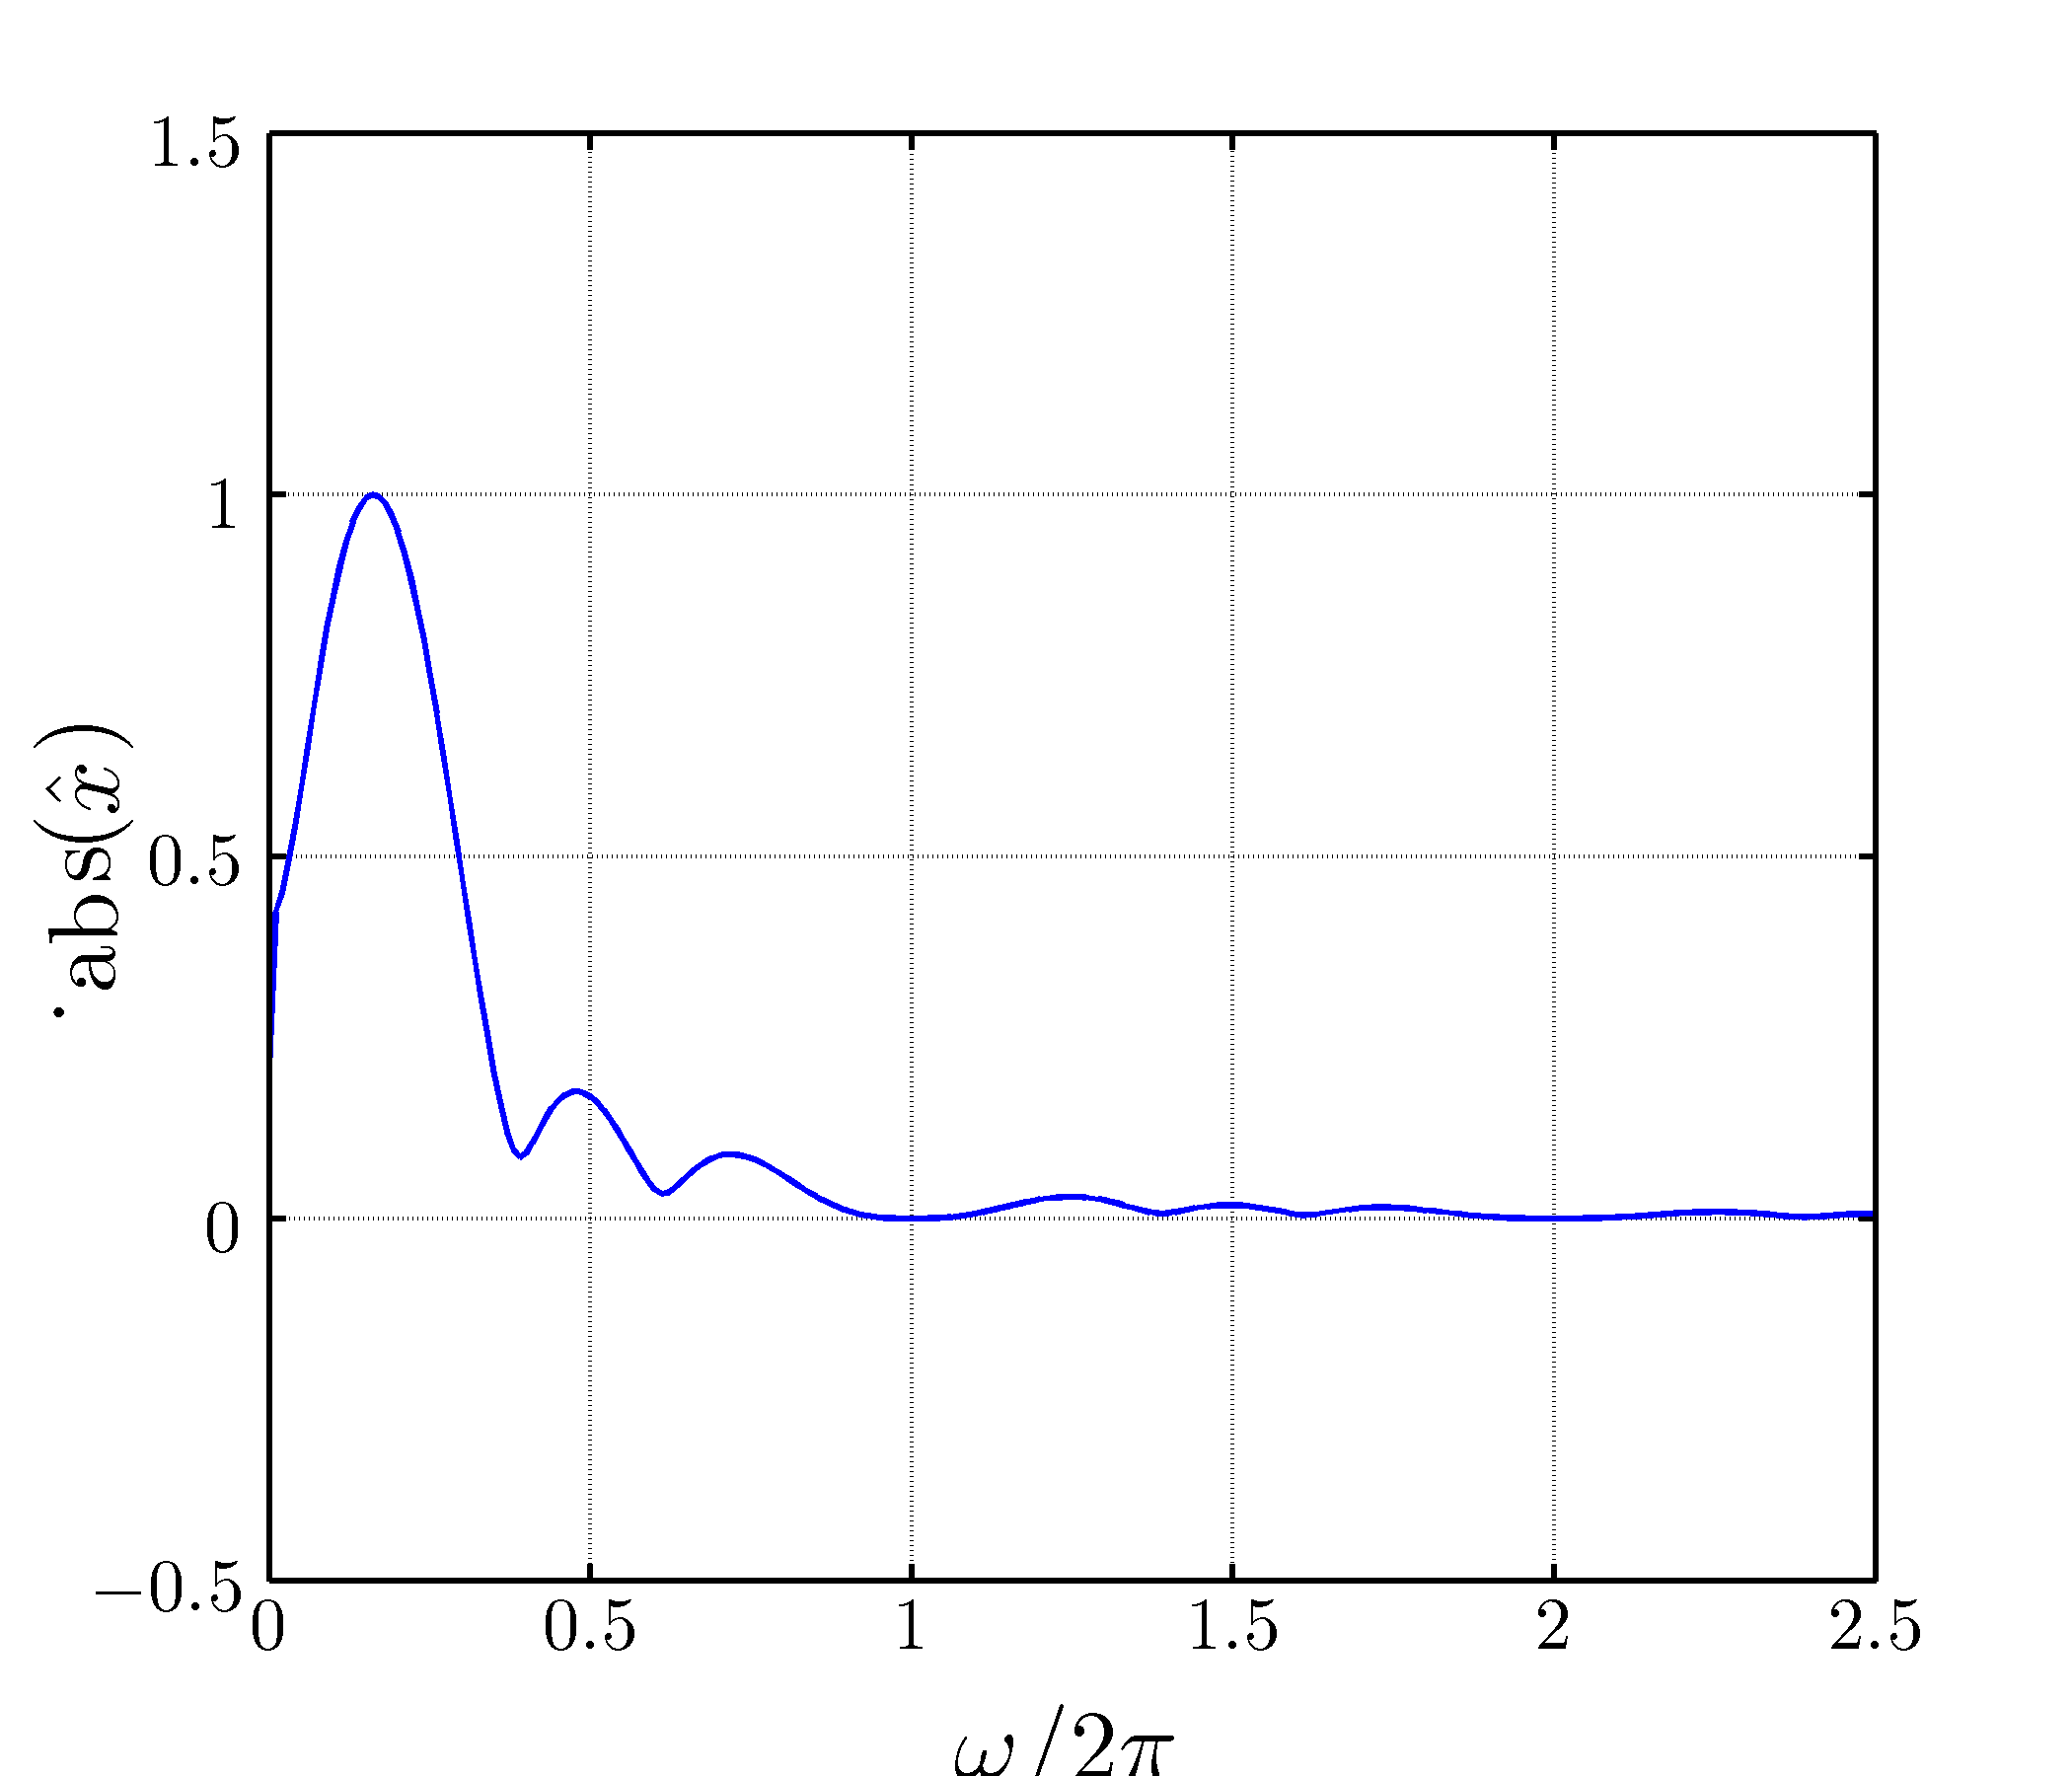
\includegraphics[width=0.45\textwidth]{./laboratorio_4/problema02_X.png}
          \end{center}
      \end{figure}

      \noindent La respuesta del sistema, representado por el bloque, al paso de
      la señal $x\left(t\right)$ será

      \begin{equation*}
        y\left(t\right) = k x\left(\tau\right) * \frac{d x\left(\tau\right)}{d \tau}
      \end{equation*}

      \noindent La transformada de Fourier de la salida $y\left(t\right)$ estará dada por

      \begin{equation*}
        \begin{split}
          \widehat{y}\left(\omega\right) & = \mathcal{F}\left(\left.k x * \frac{dx}{dt},t\right|\omega\right) \\
                                         & = k \mathcal{F}\left(x, t| \omega\right)\mathcal{F}\left(\left.\frac{dx}{dt},t\right|\omega\right) \\
                                         & = i \omega k\mathcal{F}\left(x,t|\omega\right) \mathcal{F}\left(x,t|\omega\right) \\
                                         & = i \omega k \left( - \exp\left(i \omega\right) - 1 + \exp\left(- 2 i \omega\right) \right)^{2} \mathrm{sinc}^{4}\left(\frac{\omega}{2}\right)
        \end{split}
      \end{equation*}

  \newpage
  \subsection*{Problema 3}
    \floatsetup[figure]{
      capposition=top,
      style=plain,
    }

    \noindent Halle y grafíque la transformada de Fourier de las siguientes señales:
      \begin{enumerate}[label=\alph*)]
        \item $x\left(t\right)$

          \begin{figure}[H]
            \begin{center}
              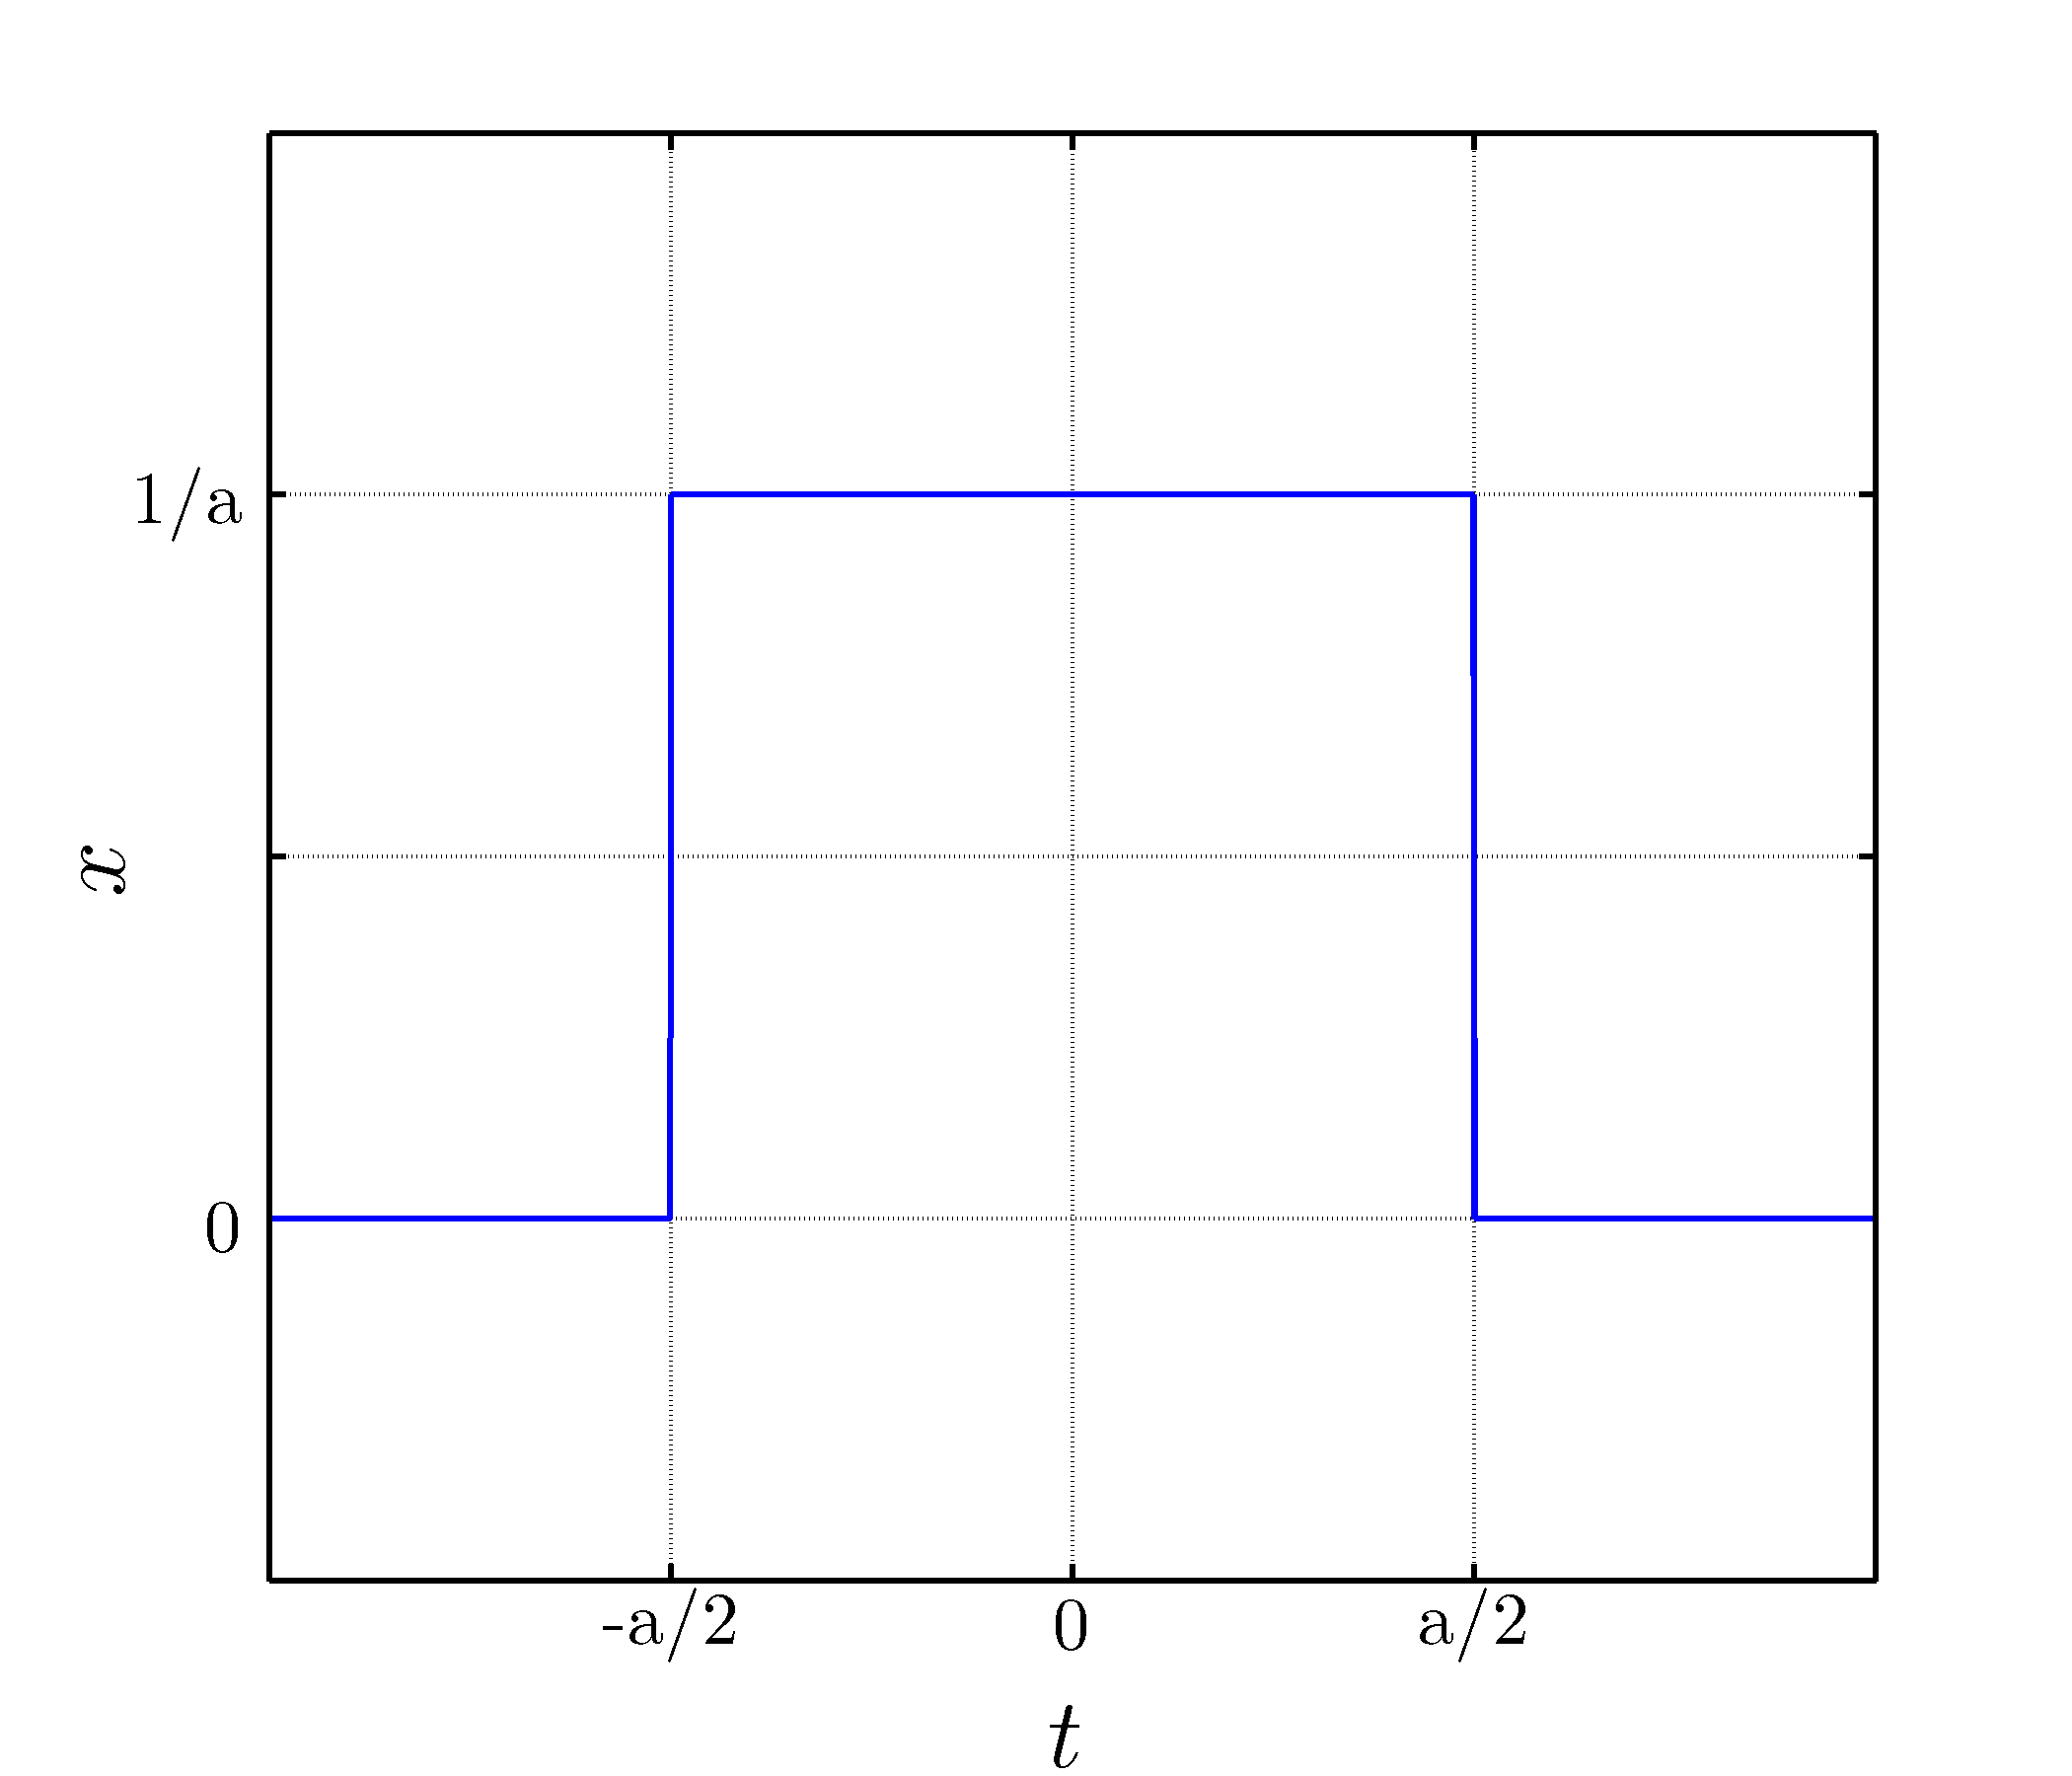
\includegraphics[width=0.5\textwidth]{./laboratorio_4/problema03_a.png}
            \end{center}
          \end{figure}\vspace{-1.5em}

        \item La función periódica mostrada en la figura:

          \begin{equation*}
            x\left(n\right) = \left\{
              \begin{array}{ccl}
                1 & ; & \mathrm{Si}\ n\ \mathrm{impar}\\
                2 & ; & \mathrm{Si}\ n\ \mathrm{par}\\
              \end{array}
            \right.
          \end{equation*}

          con $n \in \mathbb{Z}$.

          \begin{figure}[H]
            \begin{center}
              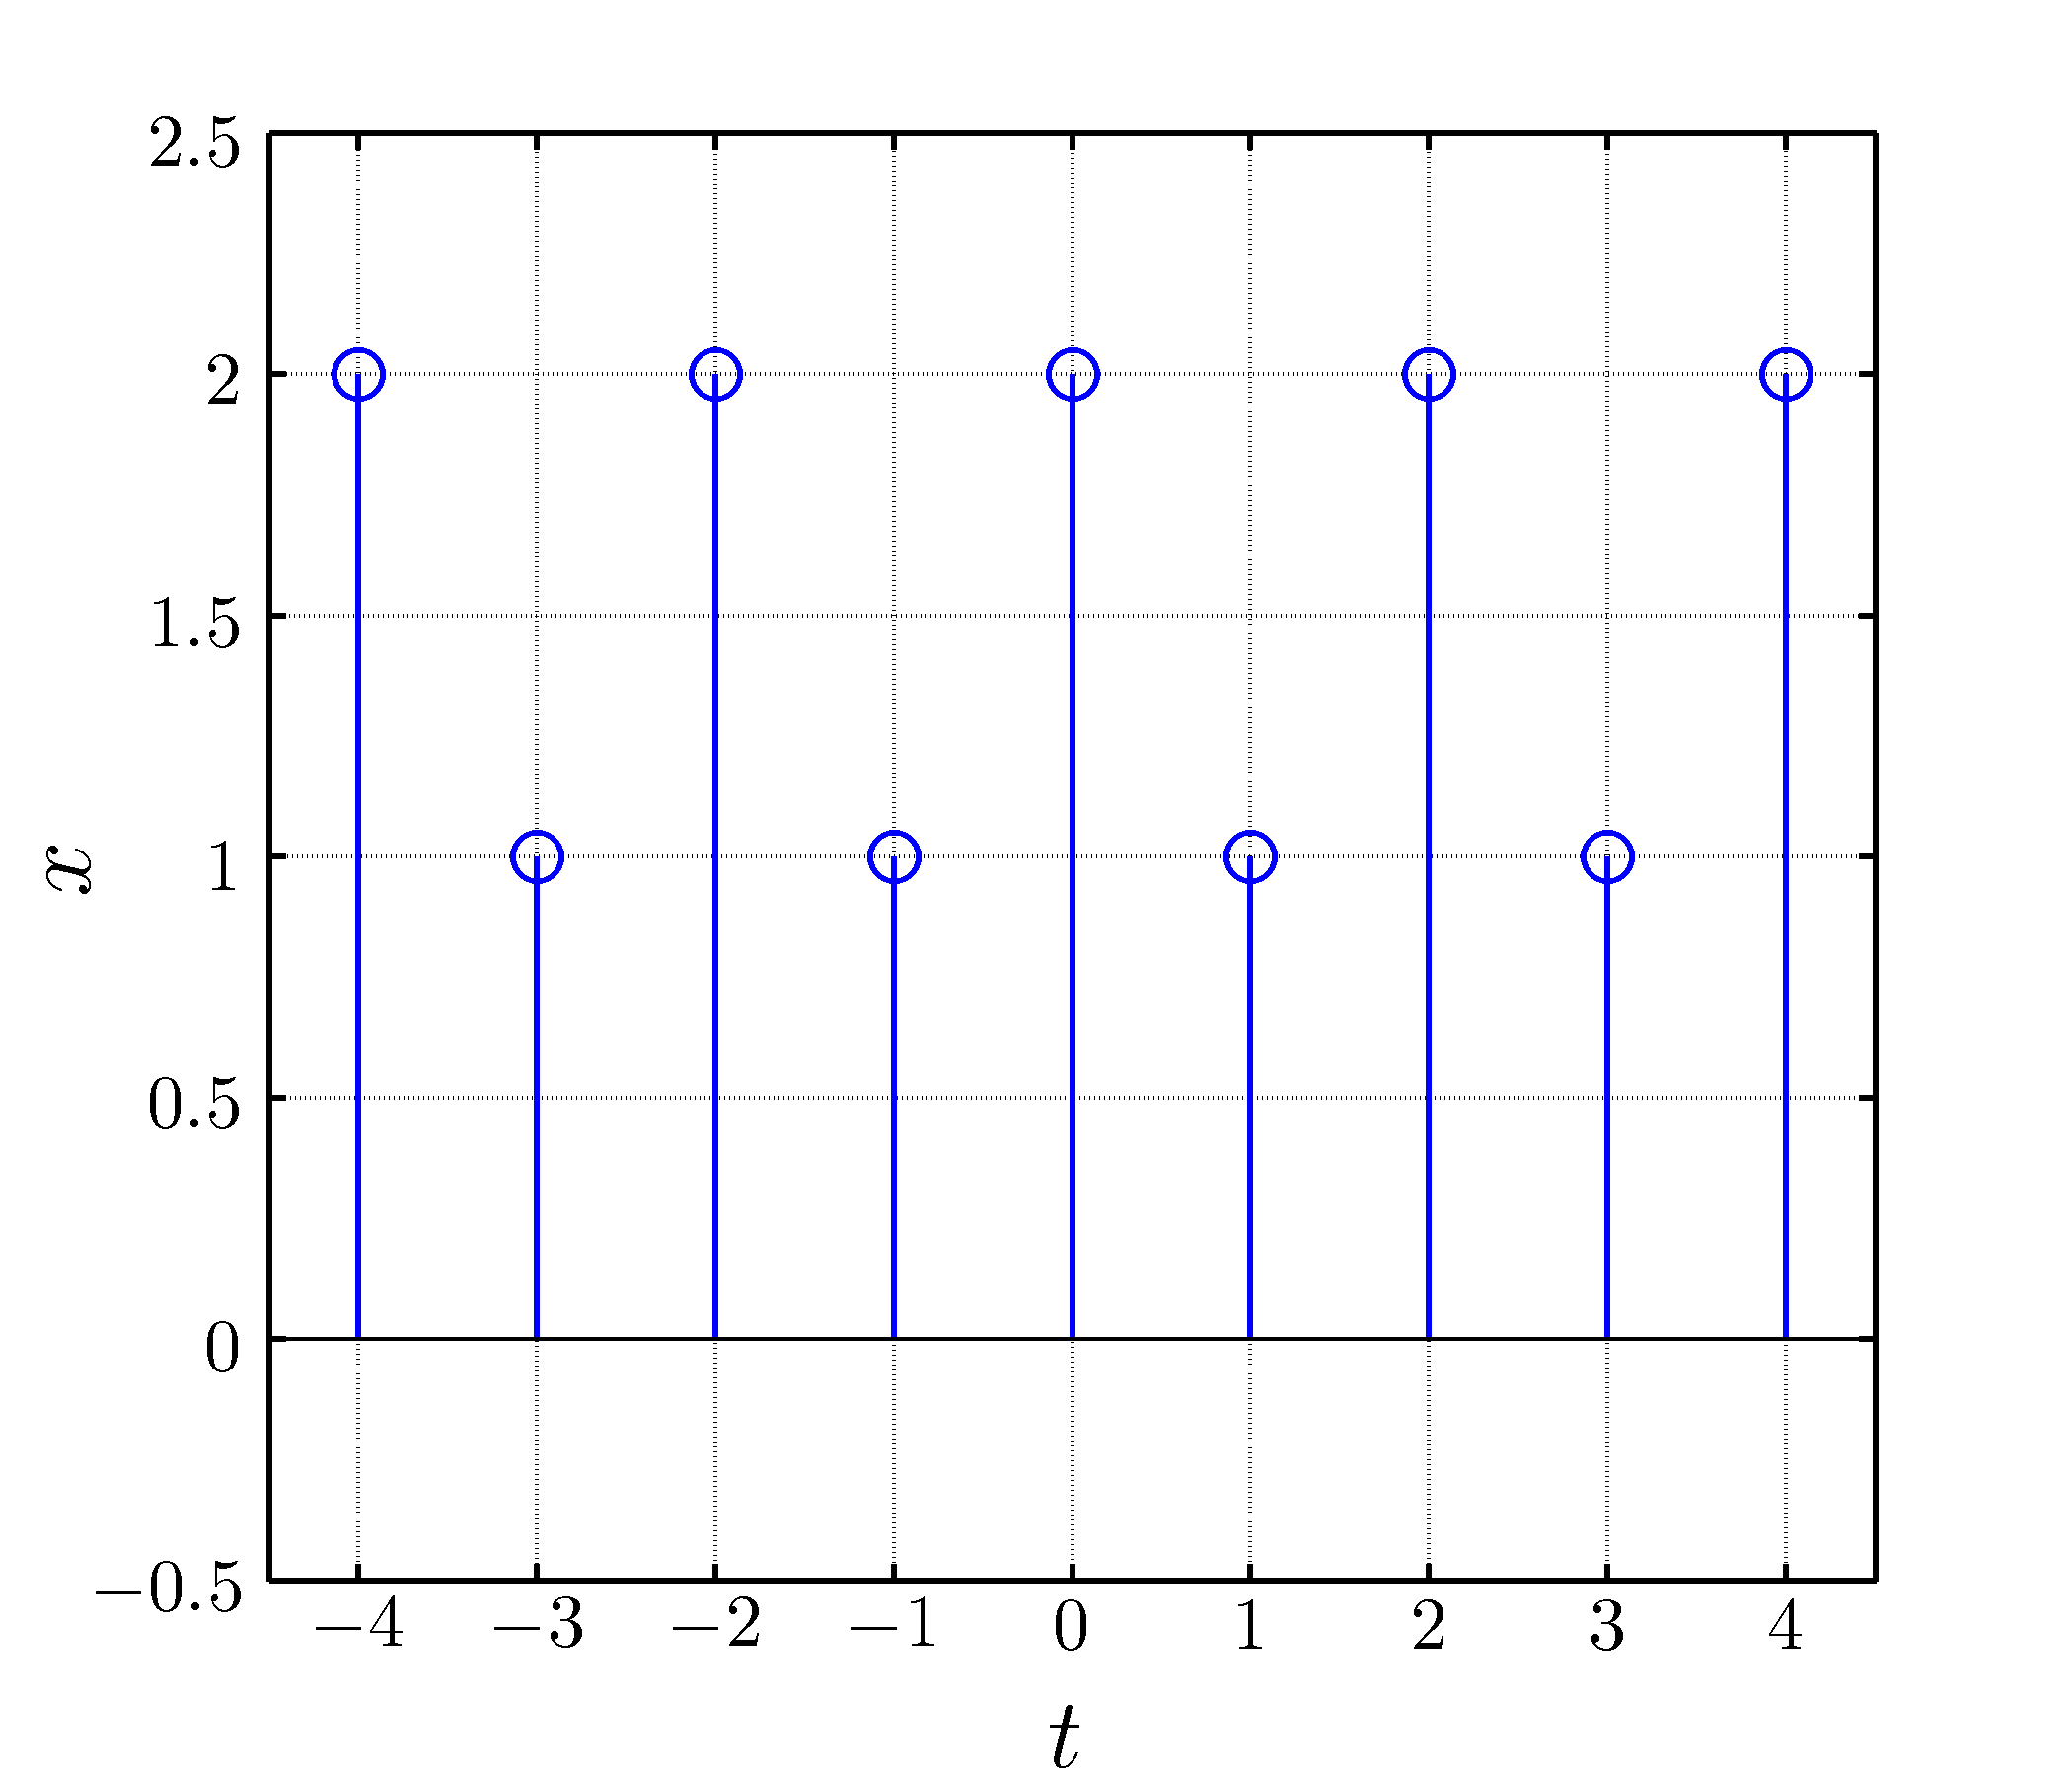
\includegraphics[width=0.5\textwidth]{./laboratorio_4/problema03_b.png}
            \end{center}
          \end{figure}\vspace{-1.5em}

        \item $f\left(t\right)$
          $$f\left(t\right) = t^2\exp\left(-\frac{t}{\tau}\right)$$

      \end{enumerate}

    \subsubsection*{Solución}
      \floatsetup[figure]{
        capposition=top,
        style=ruled,
      }

      \begin{enumerate}[label=\alph*)]
        \item Modelamos la función $x\left(t\right)$ empleando la función
          $\Theta$ de Heavisde.

          \begin{equation*}
            x\left(t\right) = \frac{1}{a}\left(
                                \Theta\left(t + \frac{a}{2}\right) -
                                \Theta\left(t - \frac{a}{2}\right)
                              \right).
          \end{equation*}

          \noindent De modo que la transformada de Fourier estará dada por

          \begin{equation*}
            \begin{split}
              \widehat{x}\left(\omega\right) & = \frac{1}{a}\left(
                                                   \mathcal{F}\left(\Theta,\left.t + \frac{a}{2}\right|\omega\right) -
                                                   \mathcal{F}\left(\Theta,\left.t - \frac{a}{2}\right|\omega\right)
                                                 \right) \\
                                             & = \frac{1}{a}\left(
                                                   \exp\left( i\omega\frac{a}{2}\right)\mathcal{F}\left(\Theta,t|\omega\right) -
                                                   \exp\left(-i\omega\frac{a}{2}\right)\mathcal{F}\left(\Theta,t|\omega\right)
                                                 \right) \\
                                             & = \frac{1}{a}\left(
                                                   -\frac{i}{\omega}\exp\left( i\omega\frac{a}{2}\right)
                                                   +\frac{i}{\omega}\exp\left(-i\omega\frac{a}{2}\right)
                                                 \right) \\
                                             & = \mathrm{sinc}\left(\frac{a\omega}{2}\right)
            \end{split}
          \end{equation*}

        % \item Modelamos la función $x\left(n\right)$ como una serie infinita de
        %   impulsos unitarios

        %   \begin{equation*}
        %     x\left(n\right) = \sum_{m=\infty}^{\infty}\left(
        %                         \delta\left(n -   m\right) +
        %                         \delta\left(n - 2 m\right)
        %                       \right).
        %   \end{equation*}

        %   \noindent De modo que la transformada de Fourier estará dada por

        %   \begin{equation*}
        %     \begin{split}
        %       \widehat{x}\left(\omega\right) & = \frac{1}{a}\left(
        %                                            \mathcal{F}\left(\Theta,\left.t + \frac{a}{2}\right|\omega\right) -
        %                                            \mathcal{F}\left(\Theta,\left.t - \frac{a}{2}\right|\omega\right)
        %                                          \right) \\
        %                                      & = \frac{1}{a}\left(
        %                                            \exp\left( i\omega\frac{a}{2}\right)\mathcal{F}\left(\Theta,t|\omega\right) -
        %                                            \exp\left(-i\omega\frac{a}{2}\right)\mathcal{F}\left(\Theta,t|\omega\right)
        %                                          \right) \\
        %                                      & = \frac{1}{a}\left(
        %                                            -\frac{i}{\omega}\exp\left( i\omega\frac{a}{2}\right)
        %                                            +\frac{i}{\omega}\exp\left(-i\omega\frac{a}{2}\right)
        %                                          \right) \\
        %                                      & = \mathrm{sinc}\left(\frac{a\omega}{2}\right)
        %     \end{split}
        %   \end{equation*}

        \item La transformada de $f\left(t\right)$ viene dada por
          \begin{equation*}
            \begin{split}
              \widehat{f}\left(\omega\right) & = \mathcal{F}\left(f,\left.-\frac{t}{\tau}\right|\omega\right) \\
                                             & = \int_{-\infty}^{\infty}t^2\exp\left(-\frac{t}{\tau}\right)\exp\left(-i \omega t\right)dt \\
                                             & = \int_{-\infty}^{\infty}t^2\exp\left(-i \left(\omega - \frac{i}{\tau} \right) t\right)dt \\
                                             & = -2 \pi \delta''\left(\omega - \frac{i}{\tau} \right)
            \end{split}
          \end{equation*}

          \noindent Donde $\delta$ es la función Delta de Dirac.
      \end{enumerate}

  \newpage
  \subsection*{Problema 4}
    \noindent Dada la señal en el dominio del tiempo:

      $$y\left(t\right) = \sin\left(t\right) + 0.25\sin\left(10t\right)$$

      \begin{enumerate}[label=\alph*)]
        \item Hacer un programa para graficar la señal para $4$ periodos, con una frecuencia de muestreo de $100\ Hz$.
        \item Hacer un programa para graficar el espectro de frecuencias de la señal.
        \item ¿Cuál es la amplitud y la frecuencia correspondiente a cada pico?
      \end{enumerate}

    \subsubsection*{Solución}

      \begin{enumerate}[label=\alph*)]
        \item El período de la función dada es de $2\pi$.
          \vspace{-2.0em}

          \setbox0=\vbox{%
            \begin{minipage}[t]{\textwidth-32pt}
                \begin{listing}[H]
                  \caption{Función $y\left(n\right)$}
                  \label{script04AY}
                  \inputminted{matlab}{./laboratorio_4/p4_y.m}
                \end{listing}
            \end{minipage}
          }%
          \makebox[\textwidth][l]{\box0}
          \vspace{-2.0em}

          \setbox0=\vbox{%
            \begin{minipage}[t]{\textwidth-32pt}
                \begin{listing}[H]
                  \caption{Función $y\left(n\right)$}
                  \label{script04AP}
                  \inputminted{matlab}{./laboratorio_4/problema04_a.m}
                \end{listing}
            \end{minipage}
          }%
          \makebox[\textwidth][l]{\box0}
          \vspace{-2.0em}

          \setbox0=\vbox{%
              \begin{minipage}[t]{\textwidth-32pt}
                \begin{figure}[H]
                  \caption{Gráfica de la función $y\left(t\right)$}
                  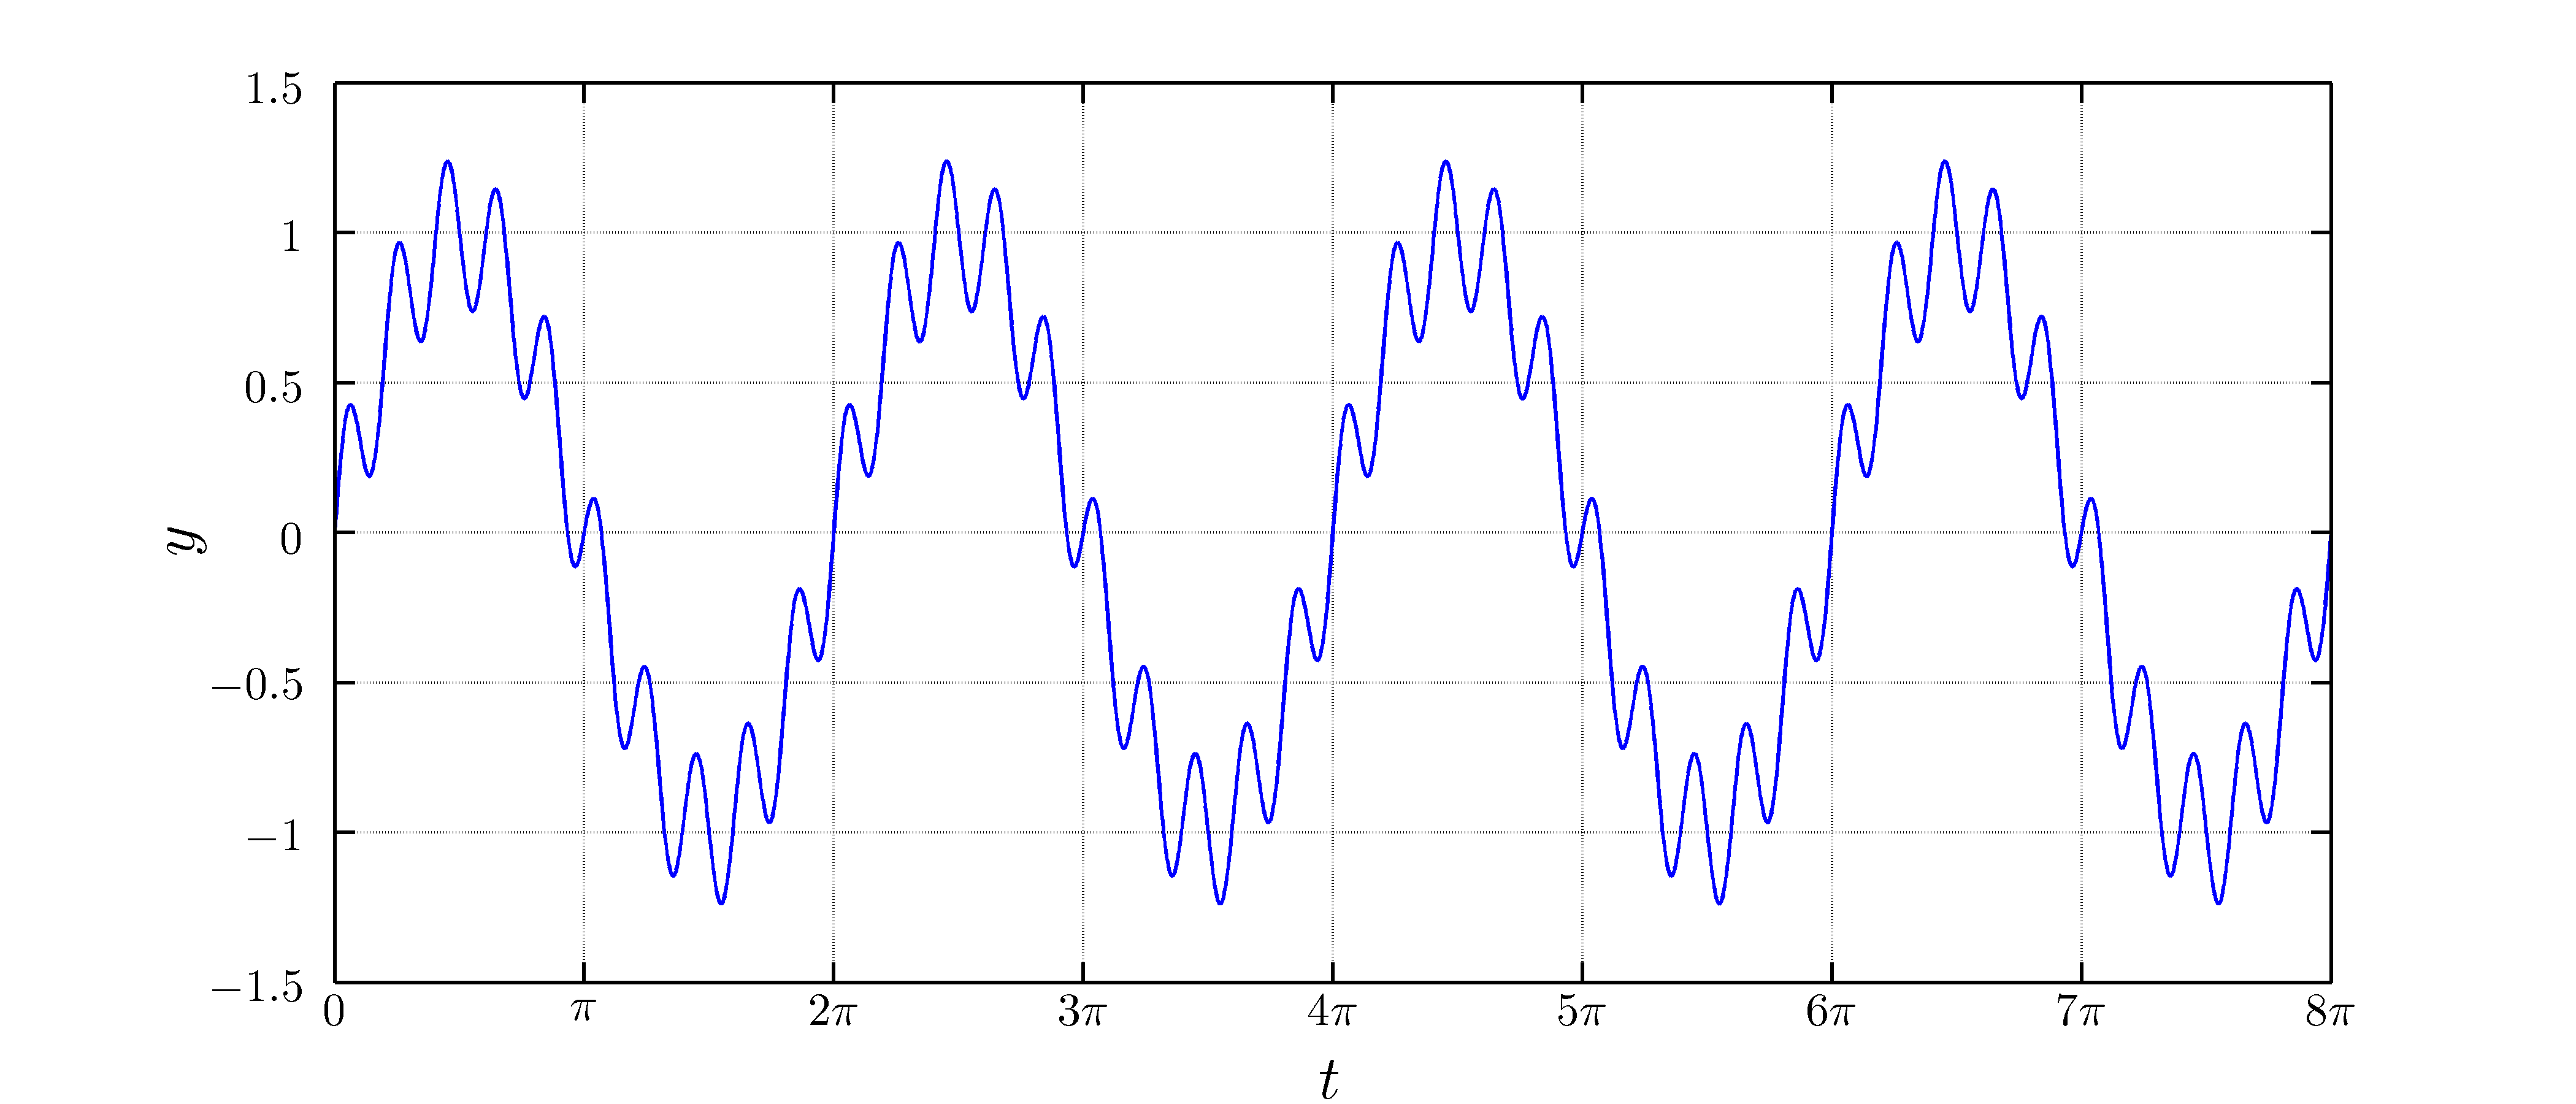
\includegraphics[width=0.95\textwidth]{./laboratorio_4/problema04_a.png}
                \end{figure}
              \end{minipage}
          }%
          \makebox[\textwidth][l]{\box0}

        \item Calculamos la transformada de Fourier y graficamos el espectro de potencias
          \vspace{-2.0em}

          \setbox0=\vbox{%
            \begin{minipage}[t]{\textwidth-32pt}
                \begin{listing}[H]
                  \caption{Función $y\left(n\right)$}
                  \label{script04B}
                  \inputminted{matlab}{./laboratorio_4/problema04_b.m}
                \end{listing}
            \end{minipage}
          }%
          \makebox[\textwidth][l]{\box0}
          \vspace{-2.0em}

          \setbox0=\vbox{%
              \begin{minipage}[t]{\textwidth-32pt}
                \begin{figure}[H]
                  \caption{Gráfica del espectro de potencias de $y\left(t\right)$}
                  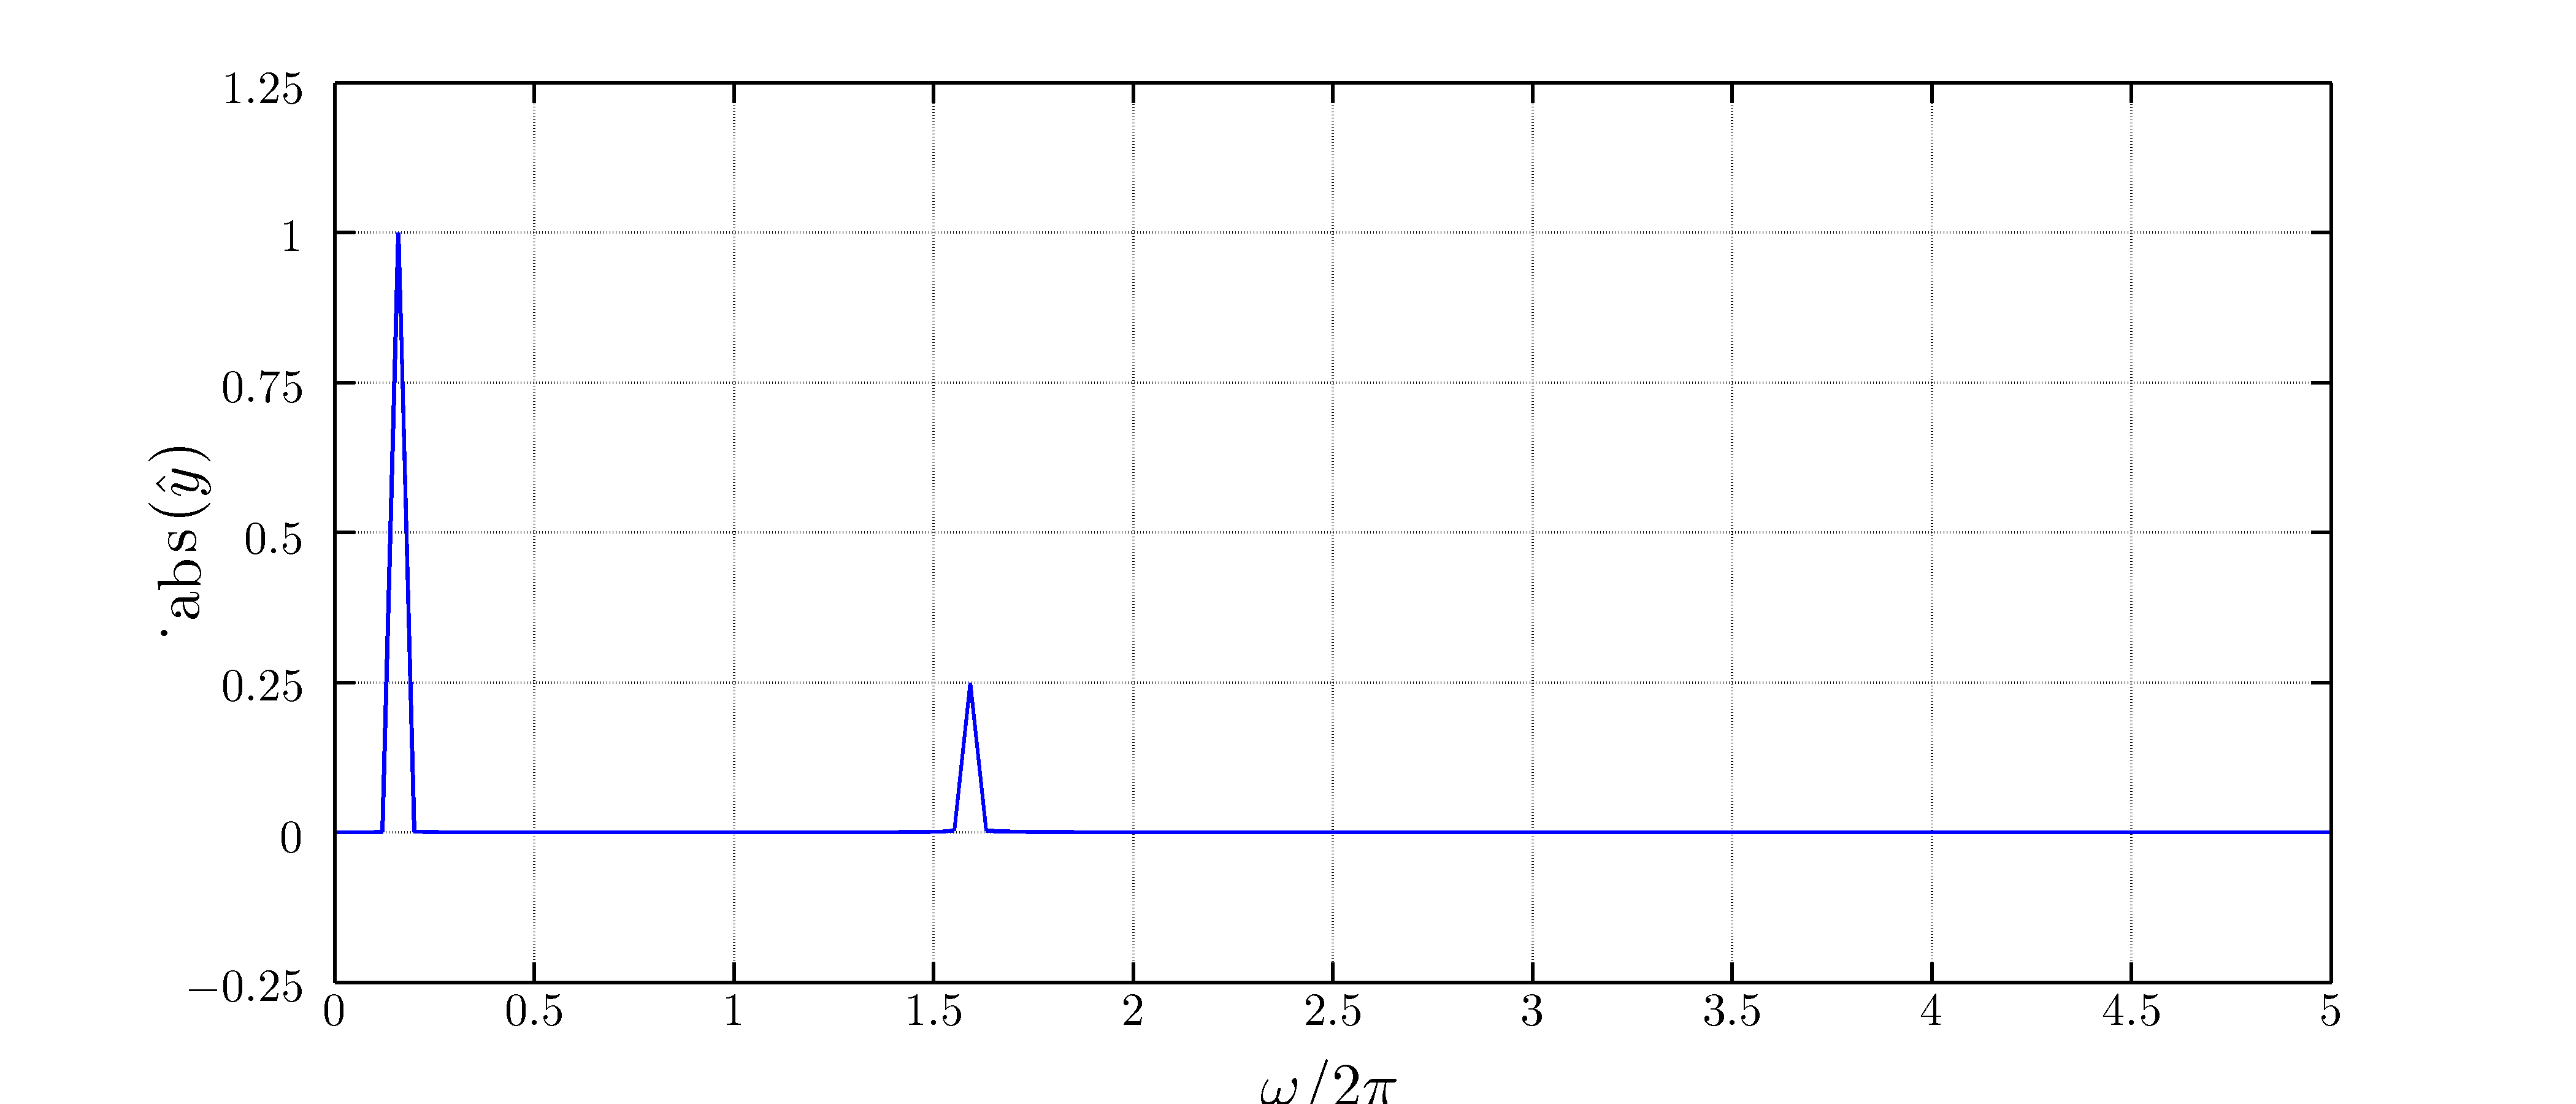
\includegraphics[width=0.95\textwidth]{./laboratorio_4/problema04_b.png}
                \end{figure}
              \end{minipage}
          }%
          \makebox[\textwidth][l]{\box0}

          \item En el espectro de potencias se encuentran dos picos con frecuencias de
            $1.5911\ \mathrm{Hz}$ y $0.1591\ \mathrm{Hz}$ con amplitudes de $0.2499$ y $0.9999$ respectivamente,
            que coinciden con los valores calculados de las amplitudes de $0.25$ y
            $1.00$ para las frecuencias $0.1592\ \mathrm{Hz}$ y $1.5915\ \mathrm{Hz}$ respectivamente.

        \end{enumerate}


  \newpage
  \subsection*{Problema 5}
    \noindent Descargue el archivo \texttt{datos.txt}\footnote{\url{http://fenlab.9k.com/pds/datos.rar}} de la web, que representa una señal de audio.
      La frecuencia de muestreo es de $F_s = 8000\ Hz$. Hacer un programa en Matlab para que realice
      lo siguiente:

      \begin{enumerate}[label=\alph*)]
        \item Hallar el número de datos N.
        \item Hallar la duración de la señal.
        \item Hallar el valor medio de la señal.
        \item Graficar la señal $x\left(t\right)$.
        \item Graficar el espectro de frecuencias.
      \end{enumerate}

    \subsubsection*{Solución}

      \begin{listing}[H]
        \caption{Script para graficar la funcion $y\left(n\right)$, su espectro de frecuencias y los parámetros solicitados.}
        \label{script05A}
        \inputminted{matlab}{./laboratorio_4/problema05.m}
      \end{listing}

      \begin{listing}[H]
        \caption{Resultado de la ejecución del \emph{script \ref{script05A}}}
        \label{script05B}
        \begin{minted}{text}
          >> problema05
          Señal y(t) contenida en el archivo 'datos.txt':
          * Cantidad de datos: 76709
          * Duracion         : 9.58863 s
          * Valor medio      : 0.00007
        \end{minted}
      \end{listing}
      \vfill
      \newpage

      \begin{figure}[H]
        \begin{center}
          \caption{Gráfica de $y\left(t\right)$}
          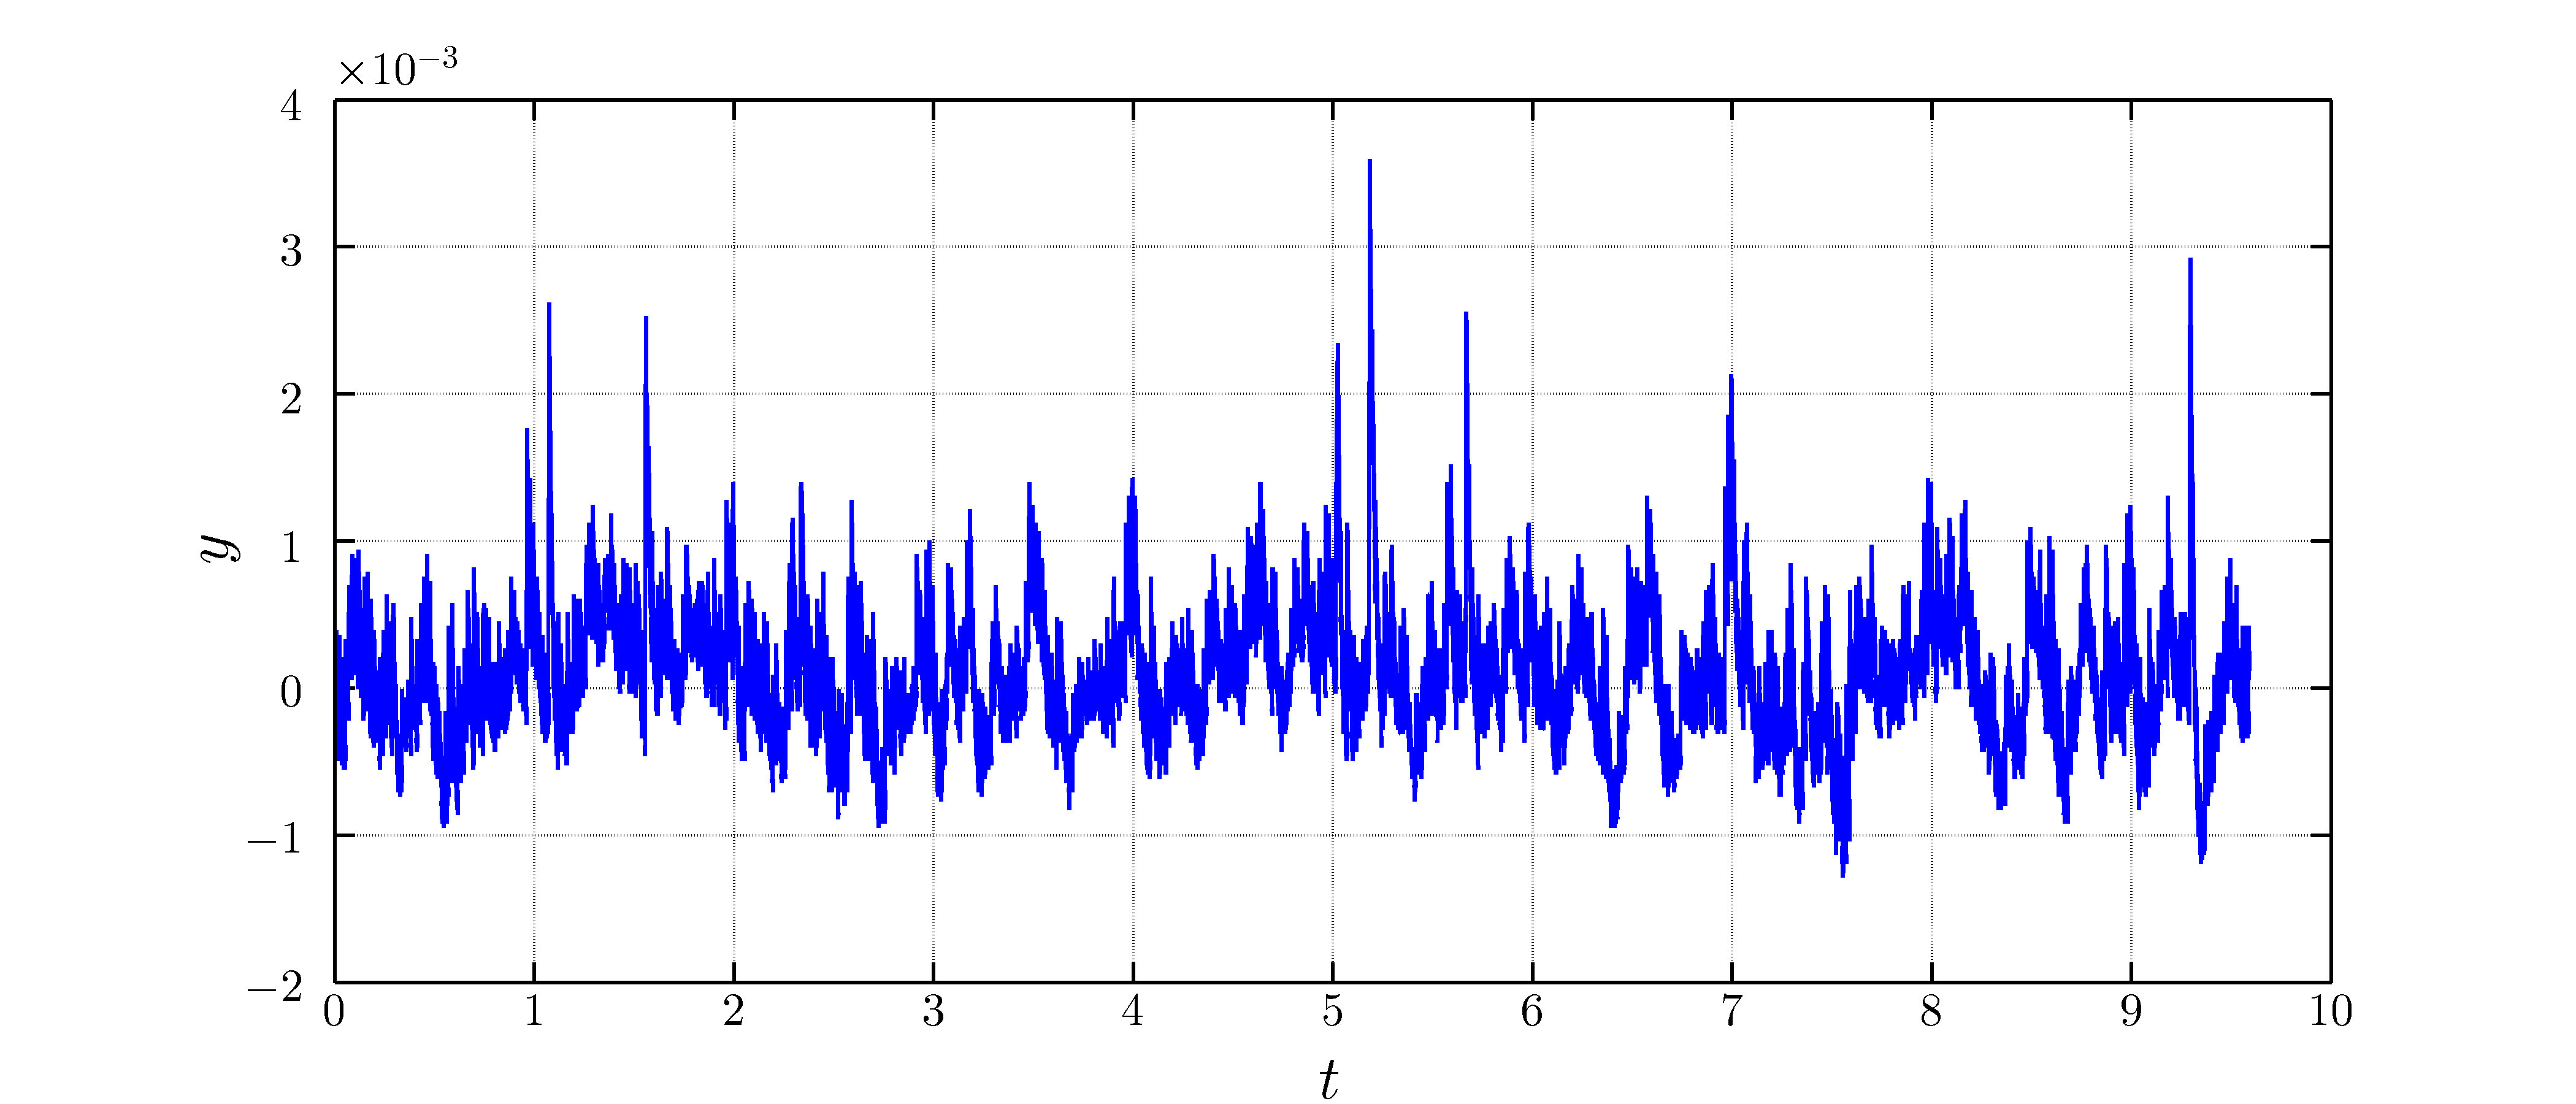
\includegraphics[width=\textwidth]{./laboratorio_4/problema05_a.png}
        \end{center}
      \end{figure}

      \begin{figure}[H]
        \begin{center}
          \caption{Gráfica del espectro de potencias de $y\left(t\right)$}
          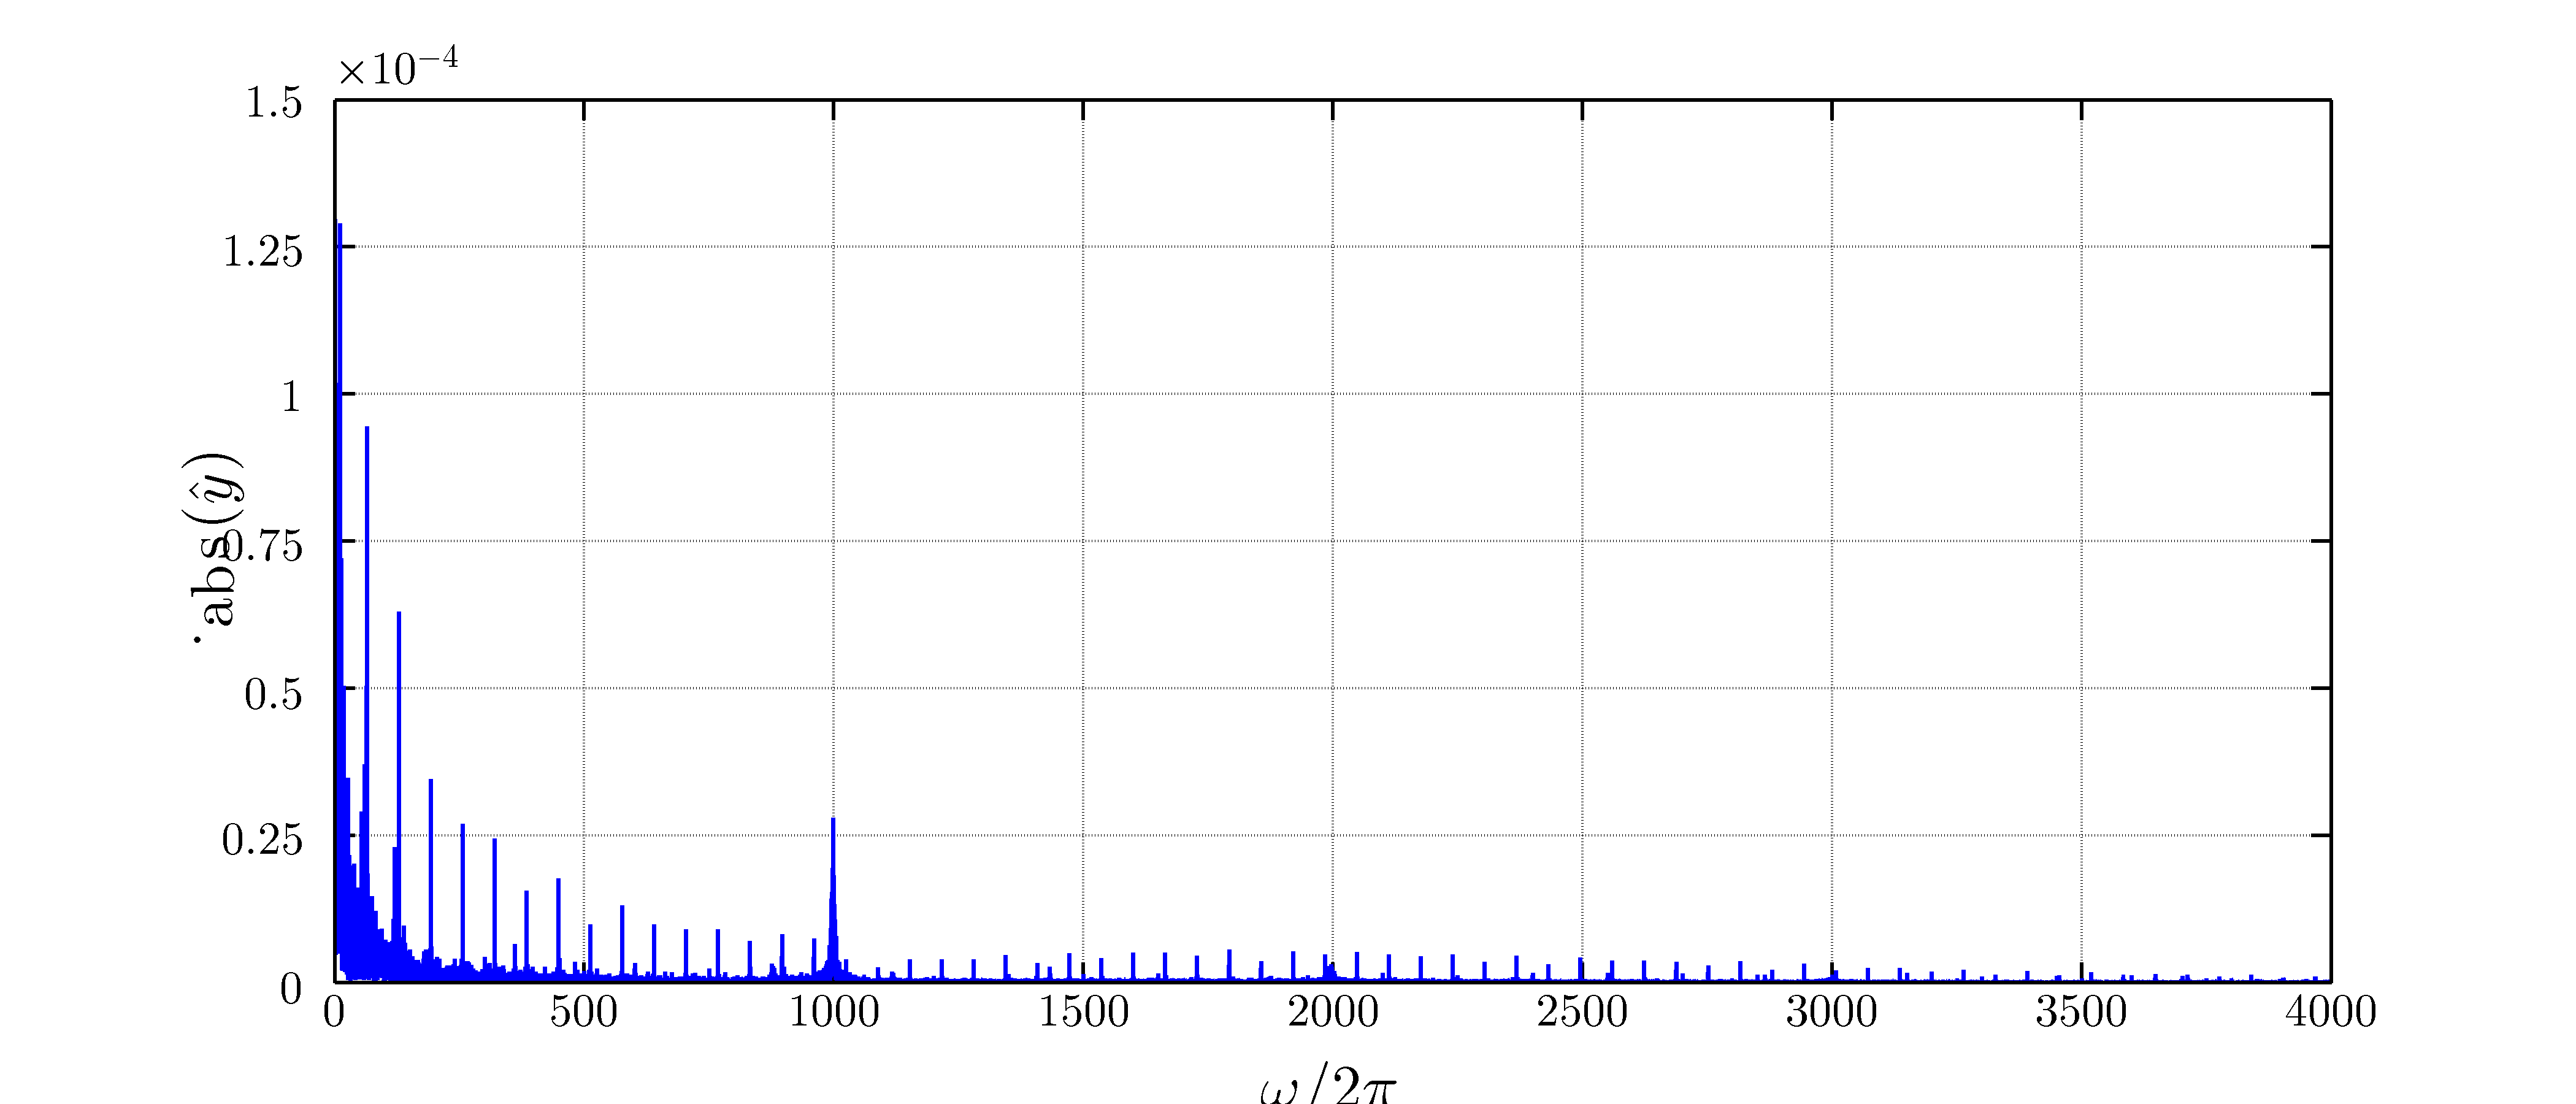
\includegraphics[width=\textwidth]{./laboratorio_4/problema05_b.png}
        \end{center}
      \end{figure}

  \newpage
  \subsection*{Problema 6}
    \floatsetup[listing]{
      capposition=top,
      style=plain,
    }

    \noindent  En \textsc{Matlab} realizar lo siguiente
      \begin{enumerate}[label=\alph*)]
        \item Calcule y grafique la transformada de Fourier de la función triángulo:
              $$x\left(t\right) = \Lambda\left(\frac{t}{2}\right)$$
        \item La integral que define la transformada de Fourier puede calcularse
          numéricamente, para cada valor de frecuencia, utilizando la suma de
          Riemman. Para subdominios de longitud T se tiene:

          $$X\left(f\right)=\sum_{N=-\infty}^{\infty}\Lambda\left(\frac{N T}{2}\right)\exp(-2 \pi j f N T )T$$

          Calcular para $T=0.8$ y para el rango de frecuencia de $0$ a $2$ con
          intervalos de $0.125$ ejecutando las siguientes sentencias en Matlab:

          \begin{listing}[H]
            \setbox0=\vbox{%
              \begin{flushright}
                \begin{minipage}[t]{\textwidth - 32pt}
                  \begin{minted}{matlab}
                    T = 0.8;
                    n = [-2:2];
                    f = [0:0.125:2];
                    X = zeros(size(f)) ;
                    for i = 1: length(f)
                        X(i) = sum(T*triangle(n*T/2).*exp(-j*2*pi*f(i)*n*T));
                    end
                  \end{minted}
                \end{minipage}
              \end{flushright}
            }%
            \makebox[\textwidth][l]{\box0}
          \end{listing}\vspace{-1.5em}

        \item Repetir para $T$ $10$ veces menor.
      \end{enumerate}

      \emph{Nota}: La función $\Lambda$ es la función triángulo
      $\Lambda\left(t\right)$ que Ud. debe implementar en \textsc{Matlab}.

    \subsubsection*{Solución}
      \floatsetup[listing]{
        capposition=top,
        style=ruled,
      }

      \noindent Implementamos la función triangulo $\Lambda\left(t\right)$
      como se indica en el \emph{script \ref{script06}}\footnote{Véase el
      problema 1 para mas detalles de las implementación}.

      \begin{listing}[H]
        \caption{Implementación de la función $\Lambda\left(t\right)$}
        \label{script06}
        \inputminted{matlab}{./laboratorio_4/triangle.m}
      \end{listing}

      \noindent La tranformada de Fourier de $x\left(t\right) = \Lambda\left(t/2\right)$
      vendrá dada por.

      \begin{equation*}
        \begin{split}
          \widehat{x}\left(\omega\right) & = \mathcal{F}\left(x,t|\omega\right) \\
                                         & = \mathcal{F}\left(\Lambda,\left.\frac{t}{2}\right|\omega\right) \\
                                         & = 2\mathcal{F}\left(\Lambda,t|2\omega\right) \\
                                         & = 2\ \mathrm{sinc}^{2}\left(\omega\right) \\
                                         & = 2\ \mathrm{sinc}^{2}\left(2 \pi f\right)
        \end{split}
      \end{equation*}

      \begin{equation*}
        \widehat{x}\left(f\right) = 2\ \mathrm{sinc}^{2}\left(2 \pi f\right)
      \end{equation*}
      \vfill
      \newpage
      \noindent Ejecutamos el \emph{script} dado en el enunciado para t = 0.8 y t = 0.08
      y graficámos $\left|\hat{x}\right|$ vs. $f$

      \begin{figure}[H]
        \caption{Gráfico de la función $\hat{x}\left(f\right)$ para $T=0.8$ y $T=0.08$}
        \begin{center}
          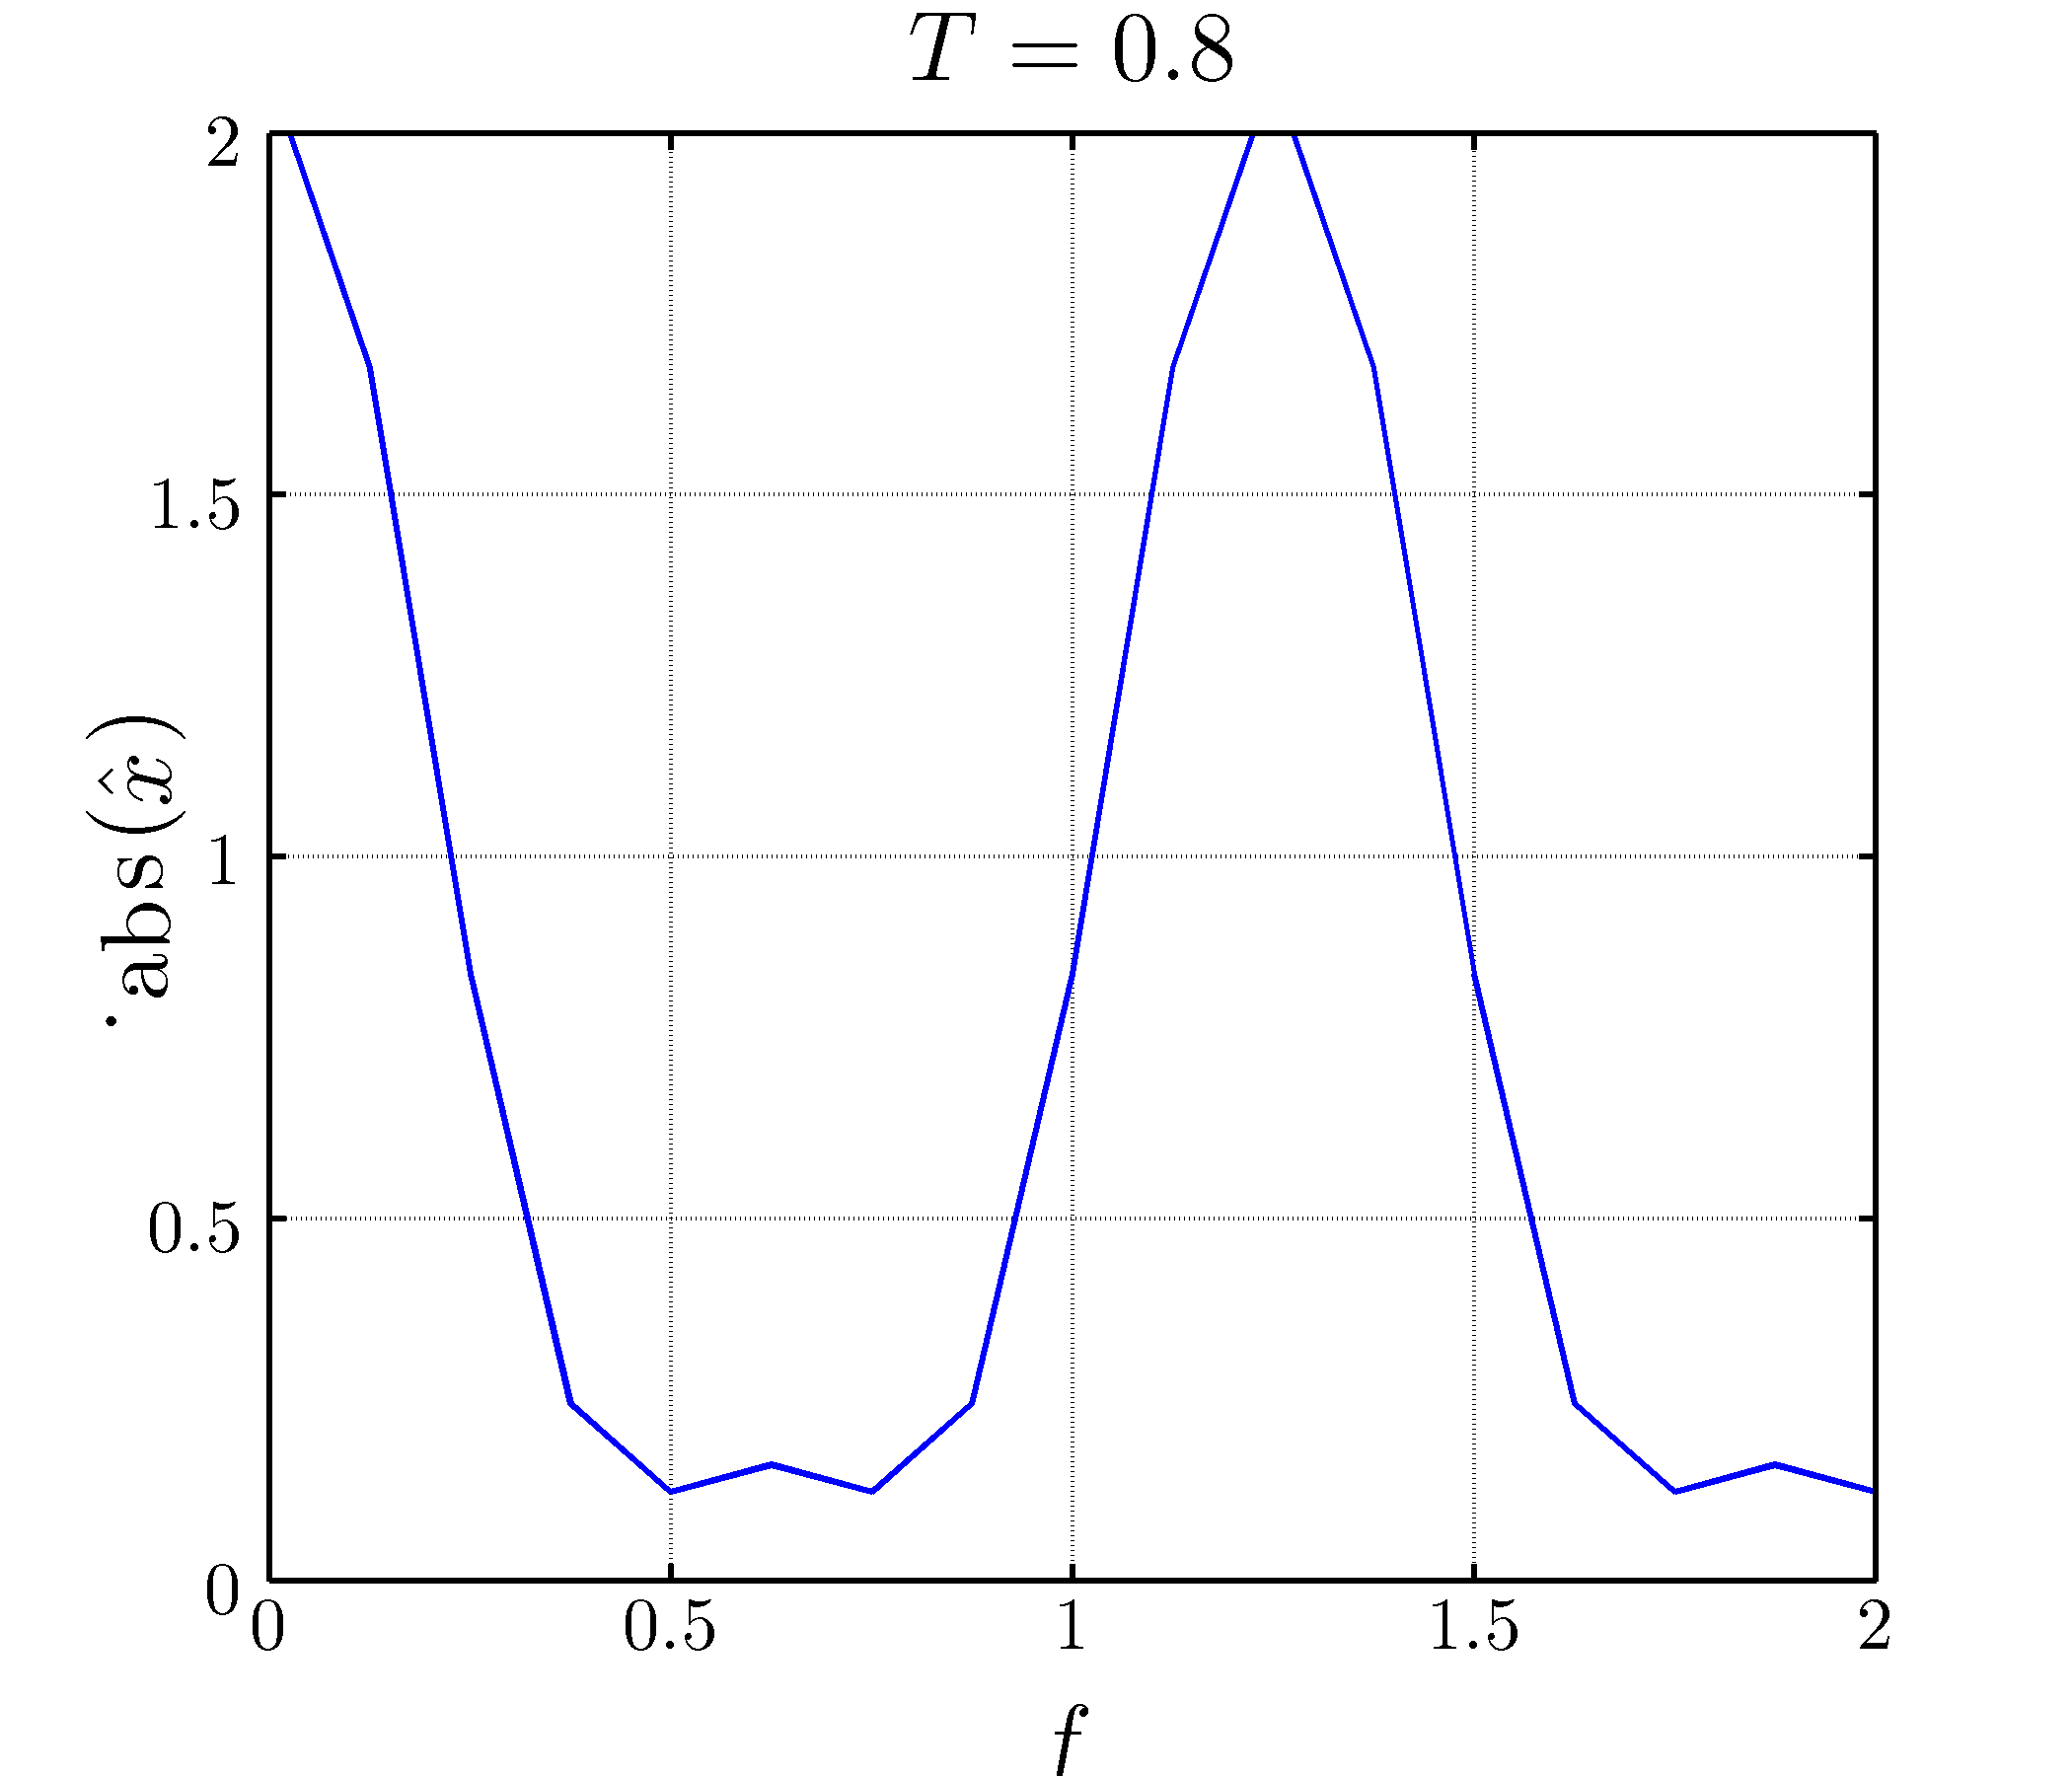
\includegraphics[width=0.45\textwidth]{./laboratorio_4/problema06_a.png}
          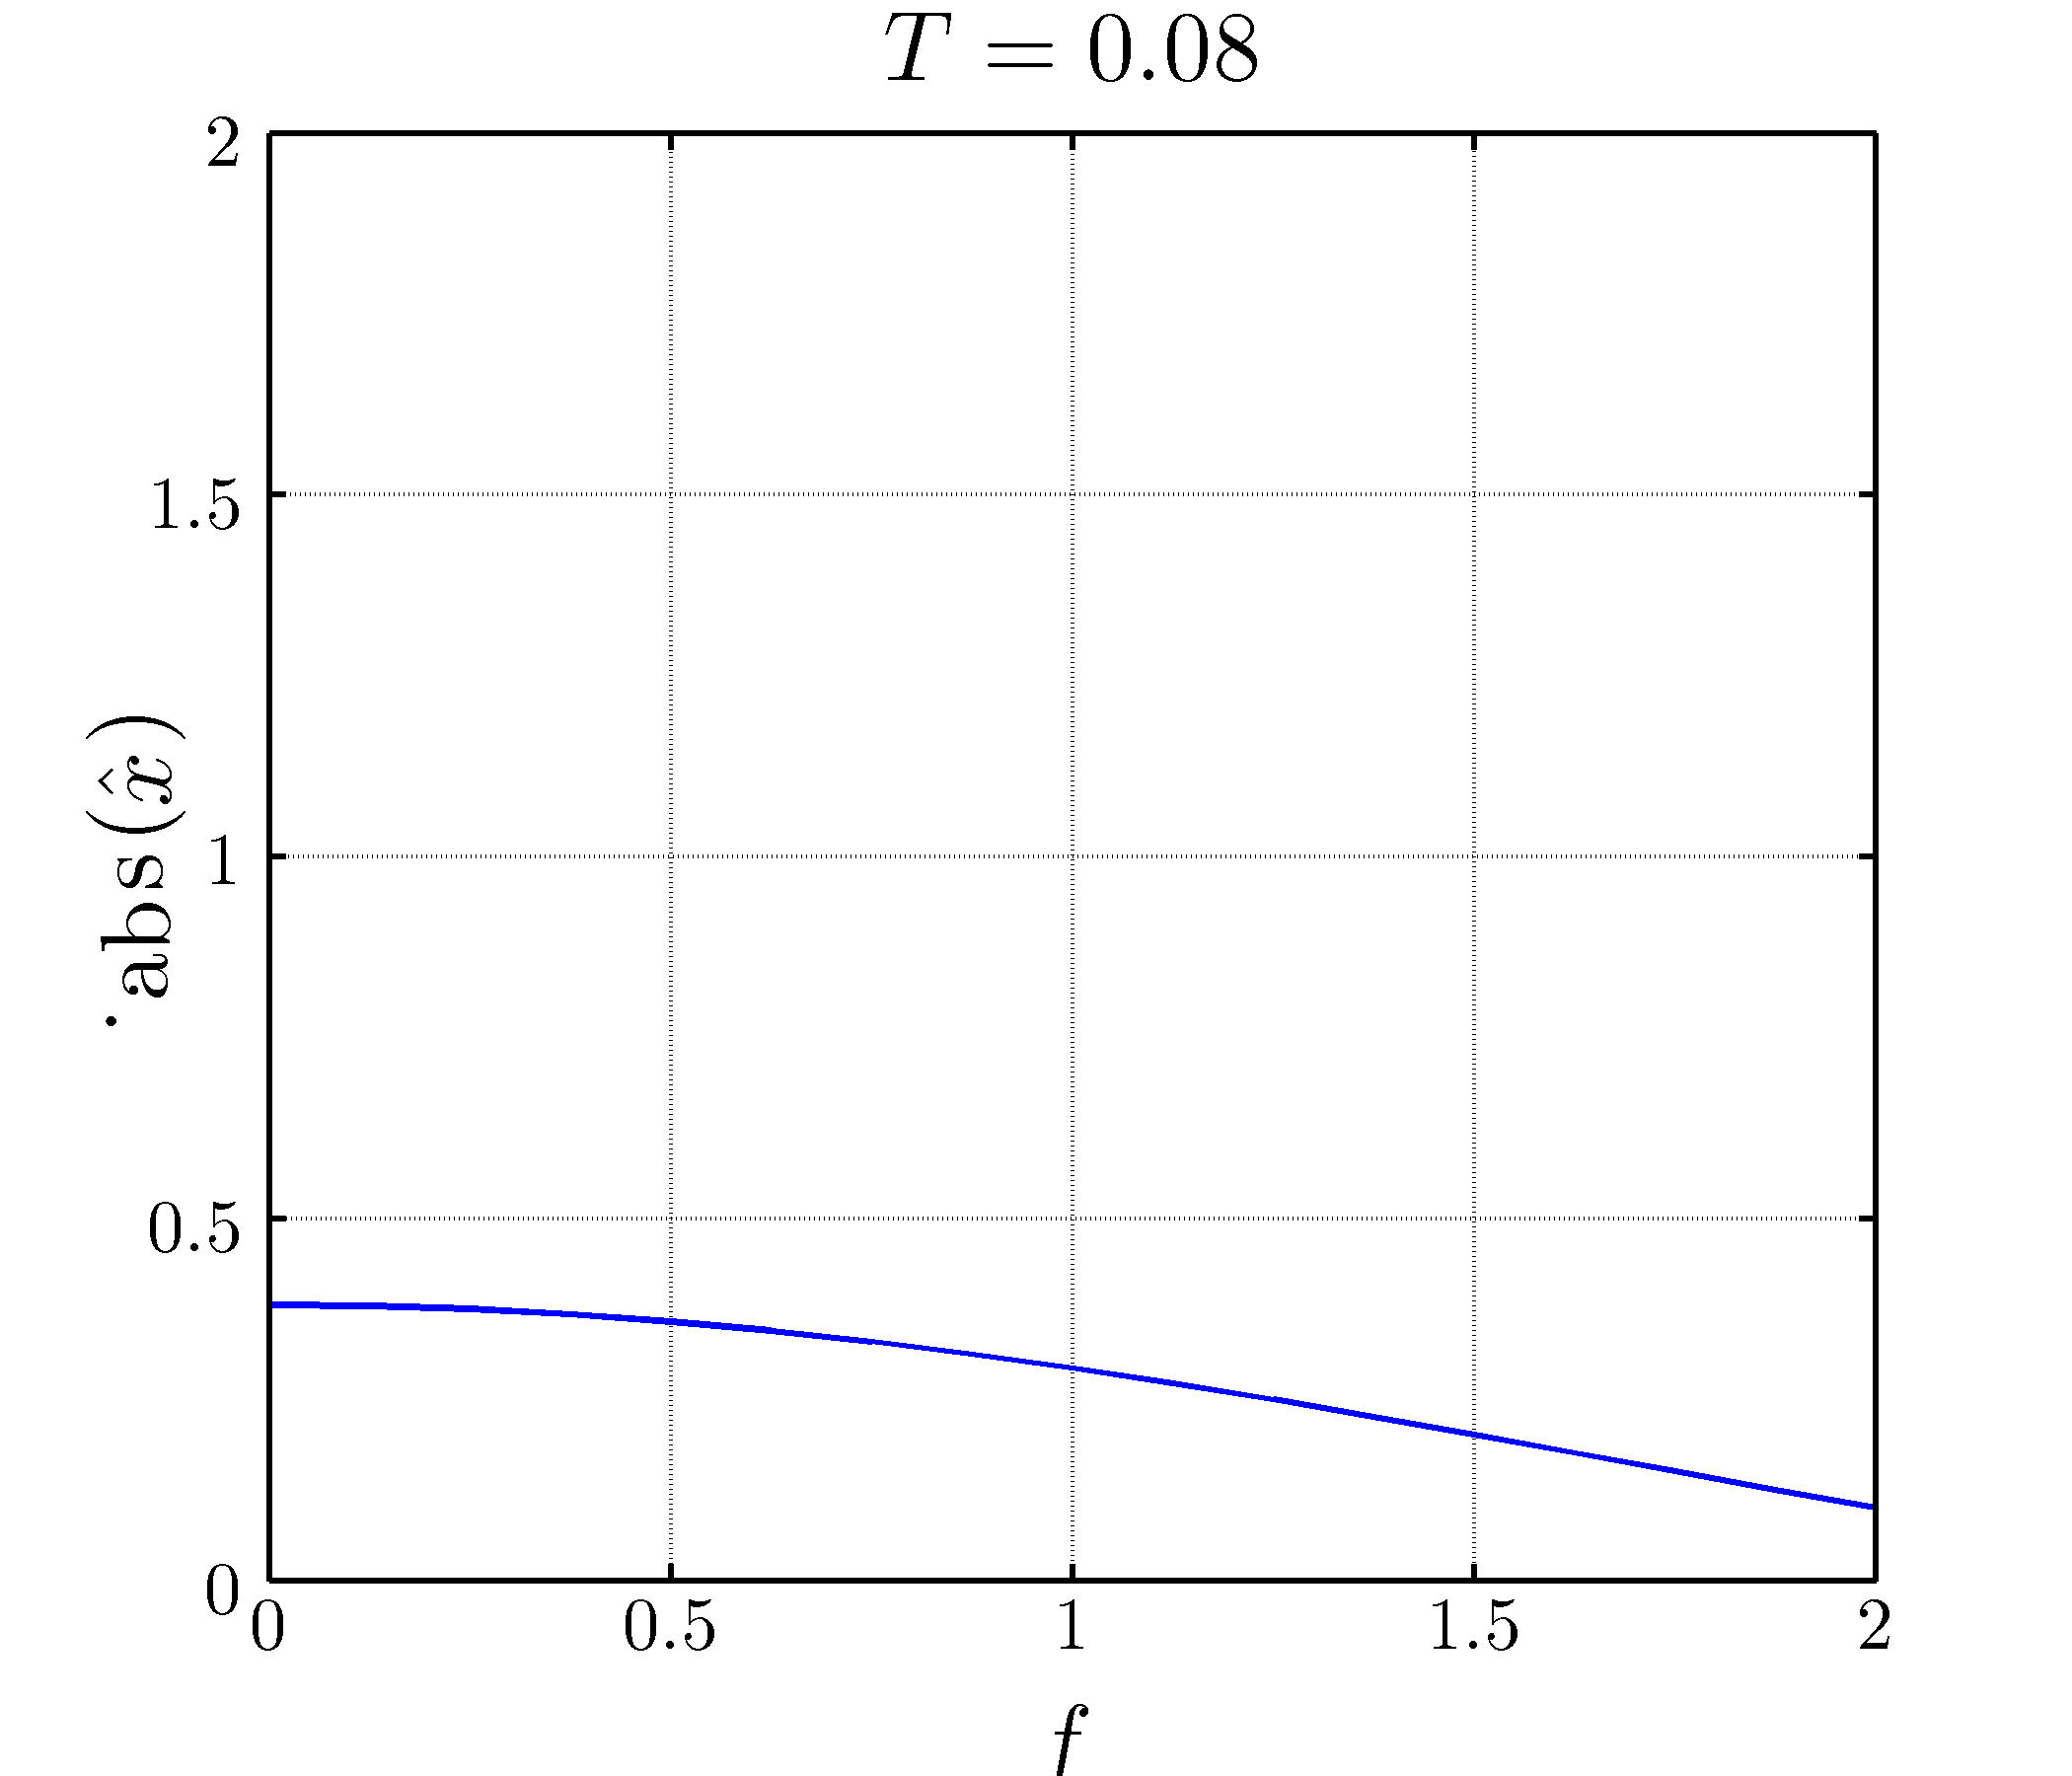
\includegraphics[width=0.45\textwidth]{./laboratorio_4/problema06_b.png}
        \end{center}
      \end{figure}

\end{document}
